\begin{figure}
\centering
\pandocbounded{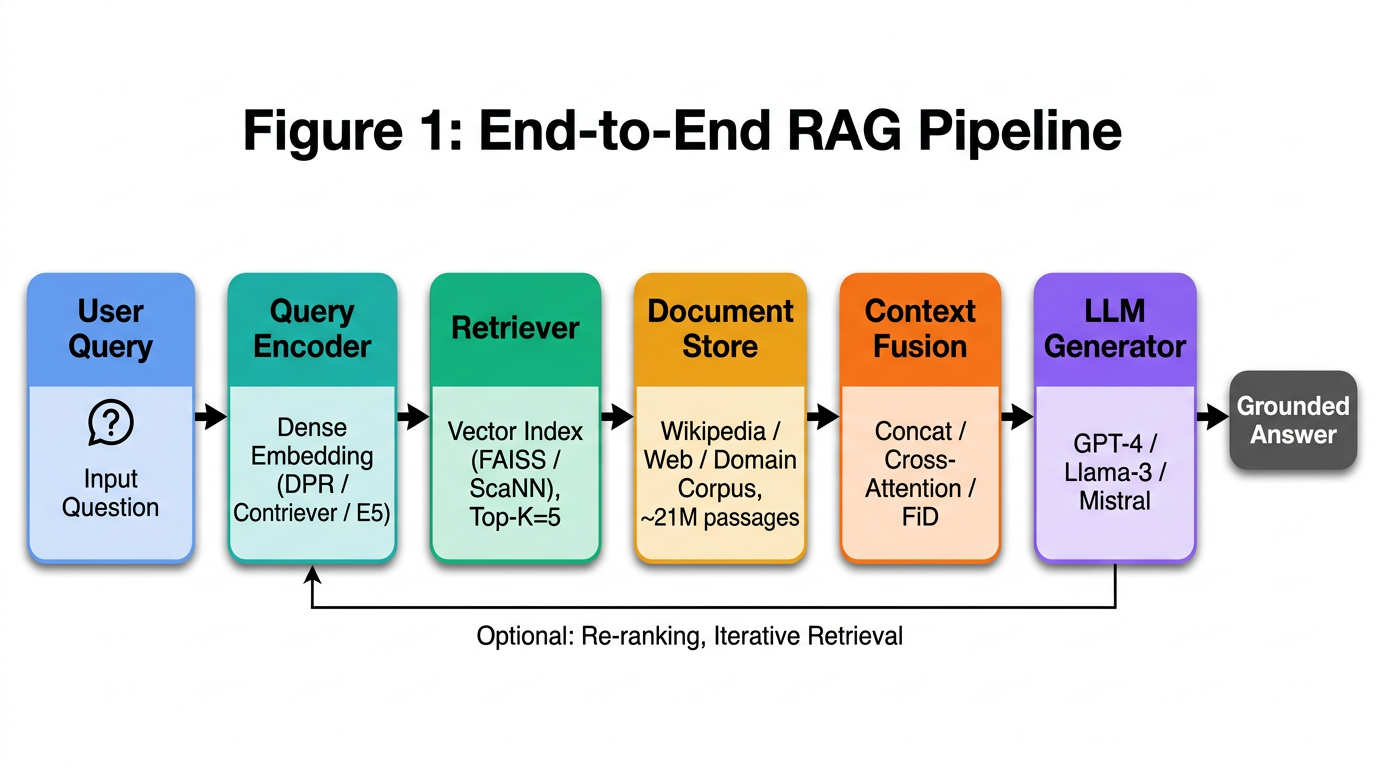
\includegraphics[keepaspectratio,alt={Figure 1. End-to-end RAG pipeline}]{./figures/Retrieval-Augmented-Generation-for-Large-Language-Models__fig_pipeline.png}}
\caption{Figure 1. End-to-end RAG pipeline}
\end{figure}

\section{Foundations and Formalization of Retrieval-Augmented Generation}\label{foundations-and-formalization-of-retrieval-augmented-generation}

\subsection{Definition, Notation, and Information-Theoretic Motivation}\label{definition-notation-and-information-theoretic-motivation}

We adopt the notation that has stabilized across the post-2020 literature. Let \(x\) denote a user query or task input, \(C\) a corpus of \(N\) candidate textual units (passages, chunks, or documents), and \(r_\eta(\cdot, x, C)\) a retriever parameterized by \(\eta\) that returns the top-\(k\) candidates \(Z = \{z_1, \dots, z_k\} \subset C\) ranked by a relevance score \(s_\eta(x, z)\). A generator \(p_\theta(y \mid x, Z)\) then produces an output sequence \(y\) conditional on the query and the retrieved evidence. Lewis et al.~(2020) define the marginal likelihood of \(y\) as \(p(y \mid x) = \sum_{z \in \text{top-}k(p_\eta(\cdot \mid x))} p_\eta(z \mid x) p_\theta(y \mid x, z)\), which preserves end-to-end differentiability when the top-\(k\) set is treated as a hard cut-off and gradients flow only through the retained documents. RAG-Sequence treats this as a per-sequence mixture, while RAG-Token re-marginalizes at every decoding step, giving a strictly more expressive family at the cost of \(k\)-fold extra compute per token. Information-theoretically, retrieval reduces the conditional entropy \(H(y \mid x)\) when the retrieved document set has high mutual information with the gold answer, which is precisely the regime in which knowledge-intensive tasks benefit from RAG. Conversely, when retrieval is irrelevant or adversarial the generator is forced to either ignore \(Z\) or be derailed by it; the noise-robustness papers of Feiteng Fang et al.~(ACL 2024) and Jinyang Wu et al.~(ACL 2025, ``Pandora's Box or Aladdin's Lamp'') quantify this regime.

The retriever is conventionally a dual-encoder that embeds queries and passages in a shared space \(\mathbb{R}^d\) with \(d \in \{384, 768, 1024, 1536\}\) for popular models such as DPR (768), Contriever (768), BGE-large and BGE-M3 (1024), E5-mistral (4096), OpenAI text-embedding-3-large (3072), and the multilingual M3-Embedding from Jianlyu Chen et al.~(Findings of ACL 2024). The relevance score is the inner product \(s_\eta(x, z) = f_\eta(x)^\top g_\eta(z)\), and the top-\(k\) search is implemented as Maximum Inner Product Search (MIPS) over a vector index, often FAISS (Matthijs Douze et al., arXiv 2401.08281, 2024), HNSW (Yu Malkov \& D. Yashunin, arXiv 1603.09320, 2016), or Milvus (Jianguo Wang et al., SIGMOD 2021). Index sizes in production reach \(10^7\) to \(10^9\) vectors at sub-50 ms latency through product quantization (PQ) and disk-based graph indexes such as DiskANN.

Three formal assumptions underlie almost all RAG analyses. \emph{Assumption A1 (Coverage):} there exists at least one \(z \in C\) that contains the answer to \(x\) verbatim or as a logical entailment; this is approximated by the Recall@\(k\) of the retriever. \emph{Assumption A2 (Faithfulness):} the generator's output is supported by some subset of \(Z\), formalized via the \emph{faithfulness} axis of RAGAS (Shahul Es et al., EACL 2024). \emph{Assumption A3 (Marginal Sufficiency):} the entropy \(H(y \mid x, Z)\) is small enough that \(p_\theta\) does not need to fall back on its parametric prior. Failures of these assumptions correspond to the principal RAG failure modes catalogued in §10.

\subsection{RAG vs.~Parametric LLMs and Long-Context Alternatives}\label{rag-vs.-parametric-llms-and-long-context-alternatives}

RAG sits between two extremes. On one side, pure parametric LLMs such as GPT-3.5 (175B), GPT-4, Llama-3-70B, Mistral-Large, and Gemini 1.0 store world knowledge implicitly and are bounded by their training cut-off; updating them requires fine-tuning or full pretraining at cost on the order of \(10^{22}\)--\(10^{25}\) FLOPs. On the other side, very-long-context models such as Claude 3.5 Sonnet (200K tokens), Gemini 1.5 Pro (1M--2M tokens), and Llama-3.1-405B-Instruct (128K) admit large evidence sets directly into the prompt, blurring the distinction between retrieval and conditioning. RAG retains three structural advantages even in the long-context era. First, \emph{non-parametric memory is editable}: a corpus can be patched in seconds by replacing a chunk, whereas the same edit in a parametric LLM costs hundreds of GPU-hours of fine-tuning and risks regression on unrelated knowledge. Second, \emph{cost scales with retrieved evidence rather than corpus size}: serving over a 100M-document index costs roughly the same per query as serving over a 1M-document index, while a long-context LLM forced to ingest the full corpus would be prohibitive. Third, \emph{citations and provenance are explicit}: the retrieved passages provide auditable trails, addressed by Tianyu Gao et al.~(EMNLP 2023) in \emph{``Enabling Large Language Models to Generate Text with Citations''}. Empirical comparisons in Boxin Wang et al.~(EMNLP 2023) on MMLU and Yunfan Gao et al.~(2023) on Natural Questions consistently show that retrieval beats long-context-only baselines once corpora exceed a few hundred thousand chunks.

The complementarity between long context and retrieval is now an active design space. LongRAG (Qi Zhao et al., EMNLP 2024) places long retrieved excerpts directly into a long-context LLM and reports gains on Long-NQ, while RAPTOR (Parth Sarthi et al., ICLR 2024) builds a hierarchical tree of recursive abstractive summaries to allow the retriever to surface coarse and fine evidence simultaneously. The ``lost in the middle'' study by Nelson Liu et al.~(TACL 2024) showed that GPT-3.5-Turbo, Claude-1, and MPT-30B each lose up to 20 absolute points of QA accuracy when the gold passage is placed in the middle of a 30-document context window, and that this U-shaped degradation persists in models trained on 100K-token contexts. This finding implies that retrieval order, chunking strategy, and reranking remain critical even when raw context length is no longer a bottleneck.

\subsection{Anatomy of a RAG Pipeline: Indexing, Retrieval, Augmentation, Generation}\label{anatomy-of-a-rag-pipeline-indexing-retrieval-augmentation-generation}

Figure 1 summarizes the canonical pipeline. The four stages --- \emph{indexing}, \emph{retrieval}, \emph{augmentation}, and \emph{generation} --- are analyzed in turn throughout the rest of this survey. Indexing is the offline step in which a corpus \(C\) is parsed, cleaned, chunked into spans of typically 200--512 tokens (often 256), embedded by an encoder, and stored in a vector index. Chunk size is a major hyperparameter: shorter chunks improve retrieval precision but inflate index size and dilute context; longer chunks reduce index size but place a heavier integration burden on the LLM. The empirical study by Xiaohua Wang et al.~(EMNLP 2024, \emph{``Searching for Best Practices in Retrieval-Augmented Generation''}) recommends chunk sizes of 256--512 tokens with 10--20 \% overlap and a 1024-dimensional embedding model such as BGE-large for English corpora.

Retrieval, the second stage, is performed online: an encoder maps the user query to the same vector space, and an ANN backend returns the top-\(k\) matches in milliseconds. State-of-the-art ANN systems such as the FAISS IVF-PQ index, HNSW with \(M=32\) and \(efSearch=128\), and Milvus's GPU-accelerated IVF achieve Recall@10 above 95 \% on 100M-vector indexes at \(<25\) ms p99 latency on a single A100 GPU. The third stage, \emph{augmentation}, splices the retrieved passages into the LLM prompt --- possibly after reranking by a cross-encoder such as ms-marco-MiniLM or ColBERTv2 (Keshav Santhanam et al., NAACL 2022), summarization (RAPTOR), filtering, or compression (Sourav Verma's contextual-compression survey, arXiv 2409.13385, 2024). The fourth stage, \emph{generation}, is the LLM forward pass; this is where the marginalization, fusion, or ensembling strategy of §5 takes effect. Latencies for end-to-end RAG over a 10M-document corpus typically decompose as 10--20 ms for query embedding, 10--40 ms for ANN retrieval, 20--80 ms for reranking, and 200--2000 ms for generation depending on the LLM size and generation length.

A useful conceptual categorization, popularized by Gao et al.~(2023) and adopted by the Wenqi Fan et al.~(KDD 2024) survey, is \emph{Naive RAG} --- single-shot retrieval and concatenation; \emph{Advanced RAG} --- query rewriting, reranking, hierarchical chunking, and self-reflection; and \emph{Modular RAG} --- composable patterns including iterative retrieval, retrieval-aware pretraining (REALM, RETRO, Atlas), and tool-augmented agents (Toolformer, AutoGen, DSPy). The survey of Yizheng Huang and Jimmy Huang (ACM Computing Surveys 2026) extends this with \emph{Agentic RAG}, in which the LLM itself orchestrates multiple retrieval calls, plans, tool invocations, and code execution. We use this four-class taxonomy throughout, and §3 deepens it along orthogonal axes such as corpus type, granularity, retriever family, and number of hops.

{\def\LTcaptype{none} % do not increment counter
\begin{longtable}[]{@{}
  >{\raggedright\arraybackslash}p{(\linewidth - 2\tabcolsep) * \real{0.3306}}
  >{\raggedright\arraybackslash}p{(\linewidth - 2\tabcolsep) * \real{0.6694}}@{}}
\toprule\noalign{}
\begin{minipage}[b]{\linewidth}\raggedright
Term
\end{minipage} & \begin{minipage}[b]{\linewidth}\raggedright
Definition (concise)
\end{minipage} \\
\midrule\noalign{}
\endhead
\bottomrule\noalign{}
\endlastfoot
RAG & Retrieval-augmented generation: \(p(y\|x) = \sum_z p_\eta(z\|x) p_\theta(y\|x, z)\) \\
Parametric memory & Knowledge encoded in LLM weights \(\theta\) \\
Non-parametric memory & External corpus \(C\) accessed via retriever \(r_\eta\) \\
MIPS & Maximum Inner Product Search --- finds \(\arg\max_z f(x)^\top g(z)\) \\
RAG-Sequence vs RAG-Token & Marginalize per-sequence vs per-token over top-\(k\) docs \\
Naive / Advanced / Modular / Agentic RAG & Increasing levels of retrieval orchestration \\
ANN & Approximate nearest neighbor (FAISS, HNSW, ScaNN, DiskANN) \\
Faithfulness & Output supported by retrieved context (RAGAS axis) \\
Recall@k & Fraction of queries whose gold doc is in the top-\(k\) retrieved \\
nDCG@10 & Normalized Discounted Cumulative Gain at rank 10 \\
\end{longtable}
}

In the remainder of this survey we trace the historical development of RAG (§2), classify its methods (§3), dive into retrieval mechanisms (§4) and generation-side conditioning (§5), explore advanced techniques (§6) and structured/multimodal variants (§7), catalogue datasets, benchmarks, and evaluation methodology (§8), discuss domain deployments (§9), survey limitations and safety (§10), and conclude with open problems and predictions (§11).

\section{Historical Evolution from Open-Domain QA to Frontier RAG Systems}\label{historical-evolution-from-open-domain-qa-to-frontier-rag-systems}

\begin{figure}
\centering
\pandocbounded{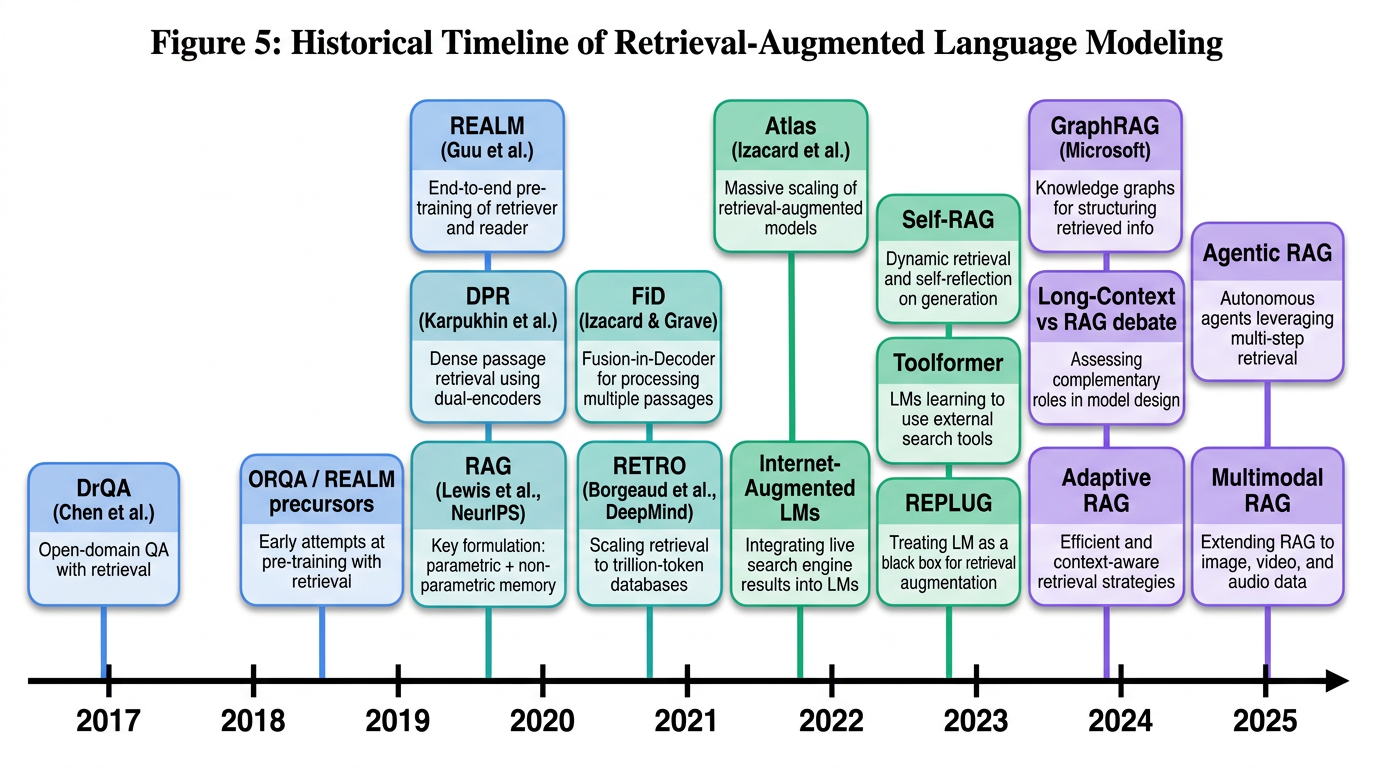
\includegraphics[keepaspectratio,alt={Figure 5. Historical timeline of retrieval-augmented language modeling}]{./figures/Retrieval-Augmented-Generation-for-Large-Language-Models__fig_timeline.png}}
\caption{Figure 5. Historical timeline of retrieval-augmented language modeling}
\end{figure}

The history of retrieval-augmented language modeling can be parsed into five distinguishable eras. Each era is marked by the emergence of a new architecture that solved a bottleneck of its predecessor and, in turn, exposed a new one. Tracing this lineage matters because most contemporary RAG systems are recombinations of components first introduced in 2017--2022; understanding the original motivations is what distinguishes a thoughtful design from a buzzword pipeline.

\subsection{Pre-Transformer Retriever-Reader Pipelines and DrQA Lineage}\label{pre-transformer-retriever-reader-pipelines-and-drqa-lineage}

The first conceptual ancestor is the \emph{retriever--reader} pipeline for open-domain question answering, exemplified by DrQA (Danqi Chen et al., ACL 2017). DrQA used TF-IDF over Wikipedia (5.1M articles) to fetch the top-5 documents and passed them to a stacked-BiLSTM reading comprehension model trained on SQuAD. Two observations made DrQA a turning point. First, \emph{non-parametric memory could already beat closed-book systems}: although DrQA's reader had only 32M parameters, the combined system answered factoid questions that no language model of the period could. Second, \emph{retrieval was the bottleneck}: the TF-IDF retriever's Recall@5 on Natural Questions was below 60 \%, capping end-to-end accuracy. This bottleneck motivated the move from sparse to dense retrieval, ultimately driving DPR.

Subsequent systems in 2018--2019 --- including BERTserini, ORQA (Lee et al., ACL 2019), and the Pyserini/Anserini stack --- refined the retriever-reader paradigm. ORQA in particular introduced \emph{Inverse Cloze Task (ICT)} pretraining, which trained a dual encoder by predicting, for a sentence, the surrounding paragraph. ICT planted the seed for self-supervised dense retrievers and is the conceptual ancestor of Contriever (Gautier Izacard et al., 2021). At the same time, the multi-hop QA dataset HotpotQA (Yang et al., EMNLP 2018) showed that single-pass retrieval was insufficient for compositional questions, planting the seed for iterative retrieval (later realized in IRCoT, FLARE, and Self-Ask).

\subsection{The 2020 Inflection Point: REALM, DPR, and the Lewis et al.~RAG Paper}\label{the-2020-inflection-point-realm-dpr-and-the-lewis-et-al.-rag-paper}

2020 was the decisive year. Three nearly simultaneous papers defined the dense-RAG paradigm. \emph{REALM} (Kelvin Guu, Kenton Lee, Zora Tung, Panupong Pasupat, and Ming-Wei Chang, ICML 2020) integrated retrieval \emph{during} masked language model pretraining: at each step, the model retrieved an evidence document, conditioned on it, and computed a marginal likelihood, allowing gradients to flow back through the retriever. REALM established that retrievers can be jointly trained with generators end-to-end, although the asynchronous index refresh (every 500 steps, on a 13M-passage Wikipedia index) was operationally fragile. \emph{DPR} (Vladimir Karpukhin et al., EMNLP 2020) demonstrated that a simple BERT-base dual-encoder, trained with a contrastive InfoNCE loss using BM25 hard negatives and in-batch negatives, beat BM25 by a wide margin on Natural Questions (78.4 vs 59.1 Recall@20) and TriviaQA. The paper's recipe --- 100M Wikipedia passages chunked at 100 words, 768-dim embeddings, FAISS IVF-PQ for serving --- became the de-facto template still used in 2026 production stacks. \emph{RAG} (Patrick Lewis et al., NeurIPS 2020) combined a frozen DPR retriever with a BART-large generator and fine-tuned them jointly with the marginalization scheme described in §1. RAG-Sequence and RAG-Token achieved state-of-the-art results on Natural Questions (44.5 EM) and Jeopardy question generation, and the paper's open-source release of code and Wikipedia indexes (21M passages) seeded the entire downstream RAG ecosystem, including HuggingFace's \texttt{transformers.RagModel} class.

A cluster of follow-up systems consolidated 2020 contributions. The Fusion-in-Decoder (FiD) model of Gautier Izacard and Edouard Grave (EACL 2021) replaced RAG's joint marginalization with independent encoding of \((x, z_i)\) pairs and a single decoder that attends across all encoder hidden states; FiD-large (770M) achieved 51.4 EM on NQ and 67.6 EM on TriviaQA, eclipsing RAG. RocketQA (Yingqi Qu et al., NAACL 2021) introduced cross-batch negatives, denoised hard negatives, and data augmentation, raising NQ Recall@5 from 71.5 to 81.1 and demonstrating the value of careful negative mining. kNN-LM (Khandelwal et al., ICLR 2020) proposed a different integration: rather than retrieve documents, it retrieved nearest-neighbor token contexts and interpolated their next-token distribution with the LM, foreshadowing token-level RAG.

\subsection{Scaling Era 2021--2024: RETRO, Atlas, Self-RAG, GraphRAG}\label{scaling-era-20212024-retro-atlas-self-rag-graphrag}

Once the dense-RAG template was established, attention shifted to scale and integration depth. \emph{RETRO} (Sebastian Borgeaud et al., DeepMind, ICML 2022; arXiv 2112.04426) was the first system to retrieve from a database of two trillion tokens --- the largest retrieval corpus ever attached to a language model at that time. RETRO chunked the input into 64-token chunks, retrieved \(k=2\) neighbors per chunk through a frozen BERT retriever, and integrated them via a novel \emph{Chunked Cross-Attention} (CCA) layer interleaved with self-attention. The headline result was that RETRO-7.5B matched the perplexity of a vanilla GPT-style 175B model on the Pile, demonstrating a 25× compute-equivalent compression in parametric size by externalizing knowledge. RETRO also established that retrieval-aware pretraining is feasible --- though expensive (\textasciitilde{}\(10^{22}\) FLOPs at training, \(5\times\) slower than vanilla LM training). \emph{Atlas} (Gautier Izacard et al., JMLR 2023) extended this to few-shot and supervised fine-tuning, jointly training a Contriever retriever with a T5-based FiD generator and reaching 42.4 \% accuracy on MMLU 5-shot using an 11B model --- a result then unmatched by closed-book LMs of the same size. \emph{Internet-Augmented Dialog} (Mojtaba Komeili, Kurt Shuster, Jason Weston, ACL 2022) showed that swapping a static index for a real-time Bing/Google API made dialog agents factually current, foreshadowing tool-augmented RAG.

The 2023--2024 era brought the LLM revolution to RAG. \emph{In-Context RAG} (Ori Ram et al., TACL 2023) showed that simply prepending retrieved passages to a frozen GPT-3 / Llama-2 prompt cuts perplexity on the Pile by up to 30 \% without any training, making RAG viable for any pretrained LLM and turning RAG into a deployment pattern rather than a model architecture. \emph{REPLUG} (Weijia Shi et al., NAACL 2024) trained the retriever via the LLM's own perplexity as a reward signal, a technique that is now standard for adapting frozen GPT-4-class LLMs. \emph{Self-RAG} (Akari Asai, Zeqiu Wu, Yizhong Wang, Avirup Sil, Hannaneh Hajishirzi, ICLR 2024) added reflection tokens --- \texttt{{[}Retrieve{]}}, \texttt{{[}IsRel{]}}, \texttt{{[}IsSup{]}}, \texttt{{[}IsUse{]}} --- that allow the LLM to decide whether to retrieve and to critique each retrieved document, achieving consistent gains over Llama-2-7B baselines on TriviaQA, ARC, and PubHealth. \emph{Adaptive-RAG} (Soyeong Jeong et al., NAACL 2024) introduced a complexity classifier that dispatches simple questions to closed-book inference and complex questions to multi-hop retrieval, optimizing latency--accuracy trade-offs.

The structured-RAG era opened in 2024. \emph{GraphRAG}, the Microsoft system described in Edge et al.~(arXiv 2404.16130, 2024) and surveyed by Boci Peng et al.~(arXiv 2408.08921, 2024), built a knowledge graph over the corpus by LLM-extracted entity-relation triples, then performed community detection and hierarchical summarization; on the \emph{Sufficient Coverage} metric, GraphRAG delivered 70--80 \% gains over flat vector-RAG for query-focused summarization. \emph{HybridRAG} (Bhaskarjit Sarmah et al., ACM ICAIF 2024) fused a knowledge-graph retriever with a vector retriever for financial earnings calls and reduced answer error rate by 12 \%. \emph{RAPTOR} (Parth Sarthi et al., ICLR 2024) built recursive abstractive summary trees and retrieved at multiple levels of granularity, outperforming flat chunking by 8 EM on QuALITY. The Gao et al.~(2023) survey crystallized the \emph{Naive → Advanced → Modular} taxonomy that has dominated discourse since.

The 2025--2026 frontier is characterized by three trends. First, \emph{agentic RAG} --- explored in AutoGen (Qingyun Wu et al., 2023; widely deployed by 2025), DSPy (Omar Khattab et al., ICLR 2024), and the modular-RAG analyses of Pengcheng Jiang et al.~(arXiv 2509.10697, 2025) --- places the LLM in control of when, what, and how to retrieve, often through tool-using loops with code execution. Second, \emph{trustworthy and faithful RAG} surveys by Bo Ni et al.~(arXiv 2502.06872) and Aoran Gan et al.~(arXiv 2504.14891, 2025) re-frame the field around verification, attribution, and safety. Third, \emph{temporal and multilingual RAG} benchmarks such as ChronoQA (Ziyang Chen et al., Scientific Data 2025) and MEMERAG (María Andrea Cruz Blandón et al., ACL 2025) expose persistent gaps where retrievers struggle to handle the time-sensitivity of facts and cross-language evidence.

{\def\LTcaptype{none} % do not increment counter
\begin{longtable}[]{@{}
  >{\raggedright\arraybackslash}p{(\linewidth - 6\tabcolsep) * \real{0.0201}}
  >{\raggedright\arraybackslash}p{(\linewidth - 6\tabcolsep) * \real{0.2864}}
  >{\raggedright\arraybackslash}p{(\linewidth - 6\tabcolsep) * \real{0.2261}}
  >{\raggedright\arraybackslash}p{(\linewidth - 6\tabcolsep) * \real{0.4673}}@{}}
\toprule\noalign{}
\begin{minipage}[b]{\linewidth}\raggedright
Year
\end{minipage} & \begin{minipage}[b]{\linewidth}\raggedright
Milestone
\end{minipage} & \begin{minipage}[b]{\linewidth}\raggedright
Authors / Venue
\end{minipage} & \begin{minipage}[b]{\linewidth}\raggedright
Significance
\end{minipage} \\
\midrule\noalign{}
\endhead
\bottomrule\noalign{}
\endlastfoot
2017 & DrQA & Chen et al., ACL 2017 & Retriever-reader paradigm over Wikipedia \\
2019 & ORQA, BERTserini & Lee et al., ACL 2019 & First neural dense retriever via ICT pretraining \\
2020 & REALM, DPR, RAG & Guu, Karpukhin, Lewis et al. & Birth of dense, end-to-end RAG; RAG-Seq/RAG-Tok formalism \\
2021 & FiD, RocketQA, kNN-LM, GAR & Izacard \& Grave; Qu et al.; Khandelwal et al. & Fusion-in-Decoder; cross-batch negatives; token-level retrieval \\
2022 & RETRO, Atlas, Internet-Aug & Borgeaud, Izacard, Komeili et al. & 2T-token DB; few-shot RAG; live web RAG \\
2023 & In-Context RAG, REPLUG, RAPTOR, Gao Survey & Ram, Shi, Sarthi, Gao et al. & RAG as deployment pattern; black-box conditioning; tree retrieval; canonical taxonomy \\
2024 & Self-RAG, Adaptive-RAG, GraphRAG, HybridRAG, RAGAS, FLARE & Asai, Jeong, Edge, Sarmah, Es et al. & Reflection tokens; complexity-adaptive routing; graph augmentation; first holistic RAG metric \\
2025 & MTRAG, MIRAGE, ChronoQA, RankCoT, Trustworthy RAG & Katsis, Park, Chen, Wu, Ni et al. & Multi-turn, temporal, faithfulness, ranking-CoT \\
2026 & Federated RAG, Agentic RAG, Long-Context+RAG & Joy \& Su; Huang \& Huang ACMCS & Privacy-preserving retrieval; LLM-orchestrated multi-tool RAG \\
\end{longtable}
}

Three structural lessons emerge from this trajectory. \emph{Lesson 1}: every era addressed the previous era's bottleneck --- DrQA was capped by sparse retrieval, REALM/DPR by static memory, RETRO by training cost, naive RAG by retrieval noise, and we are now at the agentic-orchestration bottleneck. \emph{Lesson 2}: the locus of innovation has migrated outward --- from reader to retriever to indexing to orchestration to evaluation --- and now circles back to retriever-aware pretraining at frontier scale, as foreshadowed by Boxin Wang et al.~(EMNLP 2023) in \emph{``Shall We Pretrain Autoregressive Language Models with Retrieval?''}. \emph{Lesson 3}: RAG's success is empirically anchored: every major contribution has been validated on Natural Questions, TriviaQA, HotpotQA, FEVER, and KILT, providing the cross-paper continuity that has allowed the field to compound progress without re-inventing benchmarks. The next two sections (§3 taxonomy, §4 retrieval) make these axes explicit.

\section{Taxonomy of RAG Methods (Naive, Advanced, Modular, Agentic)}\label{taxonomy-of-rag-methods-naive-advanced-modular-agentic}

\begin{figure}
\centering
\pandocbounded{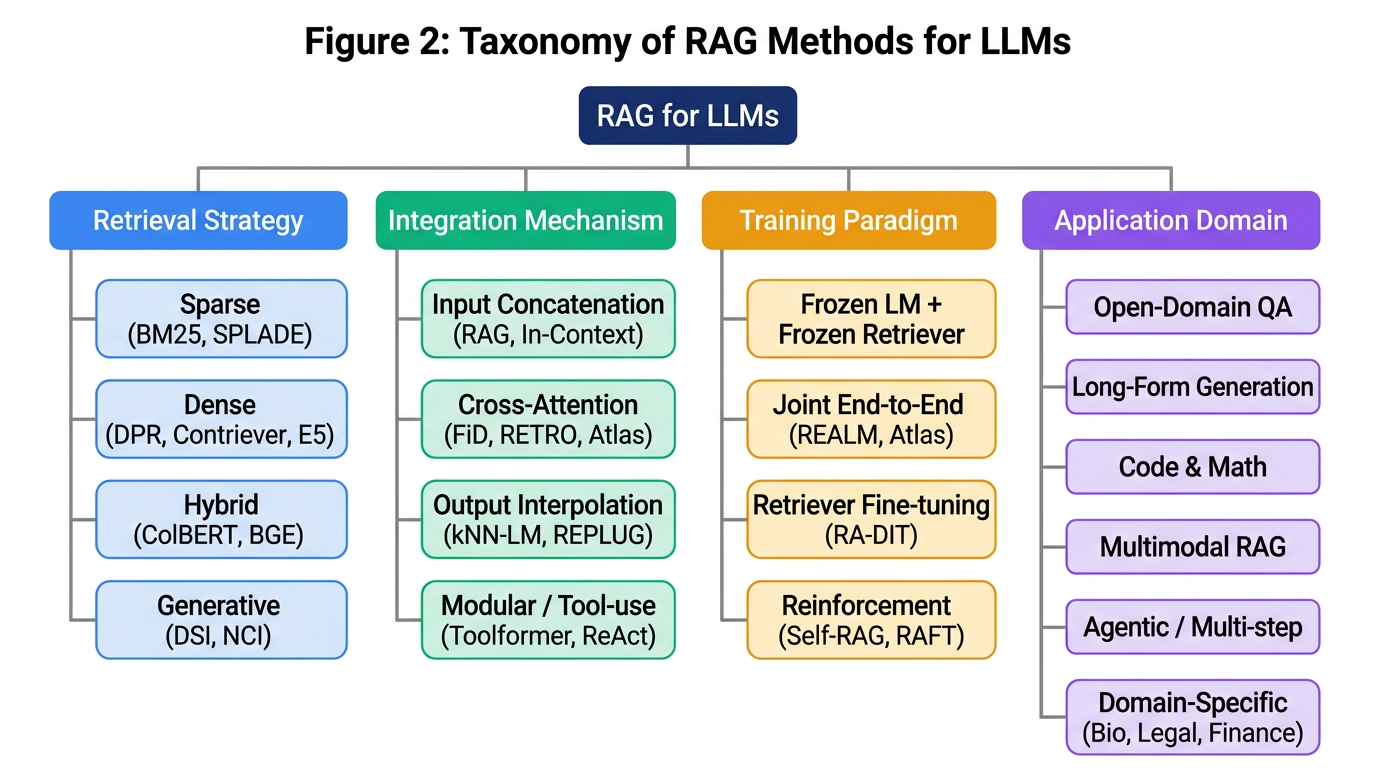
\includegraphics[keepaspectratio,alt={Figure 2. Taxonomy of RAG methods for LLMs}]{./figures/Retrieval-Augmented-Generation-for-Large-Language-Models__fig_taxonomy.png}}
\caption{Figure 2. Taxonomy of RAG methods for LLMs}
\end{figure}

Building on the historical lineage in Section 2, this section turns to a structural classification of RAG methods. This section reviews the design space of retrieval-augmented generation methods, organized along four orthogonal axes and four operational patterns. A clean taxonomy is indispensable for navigating the RAG literature, where method names proliferate and acronyms recur with conflicting meanings. We organize methods along four orthogonal axes. The first axis is the \emph{training paradigm}, which captures what is updated and what is frozen. The second axis is the \emph{retrieval timing}, which captures when retrieval happens during inference and pretraining. The third axis is the \emph{integration mechanism}, which captures how retrieved evidence is combined with the LLM's internal computations. The fourth axis is the \emph{operational pattern} --- Naive, Advanced, Modular, or Agentic. Figure 2 shows the resulting tree, and Table 3.1 summarizes the canonical members of each cell.

Representative methods include: REALM (2020, joint MLM pretraining with a learned retriever), DPR (2020, BERT dual-encoder with InfoNCE and BM25 hard negatives), RAG (Lewis et al., 2020, joint marginalization over top-\(k\) docs with RAG-Sequence and RAG-Token variants), FiD (2021, encoder-side concatenation that scales linearly in \(k\)), RETRO (2022, chunked cross-attention to a 2T-token frozen-BERT index), Atlas (2023, jointly trained Contriever + FiD-T5 reaching 56 EM on NQ at 11B), In-Context RAG (2023, frozen-LLM prompt prepend with \$\sim\$30 \% perplexity drop), REPLUG (2024, output-distribution ensembling with LM-supervised retriever tuning), Self-RAG (2024, reflection tokens {[}Retrieve{]}, {[}IsRel{]}, {[}IsSup{]}, {[}IsUse{]} for adaptive critique), Adaptive-RAG (2024, complexity-classifier routing across closed-book, single-shot, and multi-hop), FLARE (2023, confidence-gated active retrieval), RAPTOR (2024, recursive abstractive summary tree with multi-granular retrieval), GraphRAG (Microsoft, 2024, LLM-extracted KG plus community summarization), HybridRAG (2024, vector + KG fusion for finance Q\&A), HippoRAG (2024, Personalized PageRank over an entity-passage graph), G-Retriever (2024, Steiner-tree subgraph extraction), RankCoT (2025, chain-of-thought reranker), Toolformer (2023, self-supervised API-call tokens), DSPy (2024, declarative compilation of retrieval pipelines), and AutoGen (2023, multi-agent orchestration). These twenty systems collectively span every cell of the four-axis matrix and serve as anchor points for the rest of this section. In summary, the taxonomy is best read as a coordinate system: each system below occupies a unique combination of training paradigm, timing, integration mechanism, and operational pattern.

\subsection{Training Paradigms: Frozen, Retriever-Tuned, Jointly Trained}\label{training-paradigms-frozen-retriever-tuned-jointly-trained}

The first taxonomic dimension is which components carry gradient. \emph{Frozen RAG} keeps both the retriever and the LLM untouched and treats the system as a pipeline. This is the dominant pattern in production because it allows arbitrary off-the-shelf LLMs (GPT-4, Claude 3.5, Gemini 1.5, Llama-3-70B) to be paired with any embedding model. In-Context RAG (Ori Ram et al., TACL 2023) is the prototypical example: it simply prepends BM25- or BGE-retrieved passages to the prompt and reports a 30 \% perplexity drop on the Pile without any training. Frozen RAG is robust to LLM upgrades but cannot exploit feedback signals from the LLM to improve retrieval.

\emph{Retriever-tuned RAG} fine-tunes the retriever using a signal derived from the LLM, while keeping the LLM weights fixed. REPLUG (Weijia Shi et al., NAACL 2024) is the canonical instance: the retriever is updated to maximize the LLM's likelihood of the correct answer given the retrieved passage, producing a +5 EM gain on Natural Questions over BM25 with GPT-3 frozen. \emph{RankCoT} (Mingyan Wu et al., ACL 2025) extends this by training a chain-of-thought ranker that re-orders the retrieved set; the LLM's intermediate reasoning trace is the supervision signal. Retriever-tuned RAG is attractive because the retriever is small (110M--1B params) and inexpensive to train, while the LLM can remain a frozen API service.

\emph{Generator-tuned RAG} fine-tunes the LLM on retrieval-augmented data while keeping the retriever fixed. Self-RAG (Akari Asai et al., ICLR 2024) is in this category: it fine-tunes Llama-2-7B and Llama-2-13B with reflection tokens, supervised by a critic model that labels each retrieved passage as Relevant/Irrelevant and Supporting/Contradicting. Adaptive-RAG (Soyeong Jeong et al., NAACL 2024) similarly trains the LLM to choose between zero-shot, one-shot, and multi-hop retrieval. The advantage is full control over the LLM's interaction with retrieval; the cost is the loss of compatibility with closed-source LLMs.

\emph{Jointly trained RAG} updates both retriever and generator end-to-end. REALM (Kelvin Guu et al., ICML 2020) was the first such system, propagating gradients through the marginalization over top-\(k\) documents; it required asynchronous index refresh every 500 steps. Atlas (Gautier Izacard et al., JMLR 2023) refined this by using Contriever as the retriever and FiD-T5 as the generator and re-encoding the index every \$\sim\$10k training steps; with 11B parameters it reached 56 EM on NQ in the few-shot setting. RETRO (Sebastian Borgeaud et al., 2022) is also jointly trained but only updates the LM (the retriever is a frozen BERT). Joint training delivers the best end-to-end performance per parameter but is operationally heavy.

\subsection{Retrieval Timing: One-Shot, Iterative, Pre-Training Integrated}\label{retrieval-timing-one-shot-iterative-pre-training-integrated}

The second axis is \emph{when} retrieval is invoked. \emph{One-shot retrieval} --- retrieve once at the beginning of generation --- is the simplest pattern and matches Lewis et al.~(2020), DPR+FiD, and most production deployments. It is sufficient for single-hop QA but is fundamentally incapable of multi-hop reasoning, where the second retrieval depends on the first answer. \emph{Iterative retrieval} addresses this. IRCoT (Trivedi et al., ACL 2023) interleaves chain-of-thought reasoning with new retrievals after each step; Self-Ask (Press et al., 2023) issues sub-questions; FLARE (Jiang et al., 2023) triggers retrieval whenever the LLM's next-token confidence drops below a threshold. RAPTOR (Parth Sarthi et al., ICLR 2024) instead pre-computes a hierarchical summary tree and retrieves at multiple granularities in a single shot, blurring the line between iterative and structured retrieval.

\emph{Pre-training-integrated retrieval} embeds retrieval into the LM's training objective. REALM, RETRO, and Atlas are all in this class, with the practical distinction that RETRO is the only one that scales the retrieval database to two trillion tokens, requiring a custom MIPS infrastructure. Boxin Wang et al.~(EMNLP 2023) explicitly compared retrieval-aware pretraining to retrieval-aware fine-tuning at GPT-3 scale and found that pretraining-integrated retrieval delivers roughly 4 perplexity points and 6 EM points of additional gain on Natural Questions over the same model trained without retrieval, validating the RETRO/Atlas line of investment.

\subsection{Integration Mechanism: Concatenation, Cross-Attention, Distribution Interpolation}\label{integration-mechanism-concatenation-cross-attention-distribution-interpolation}

The third axis describes how retrieved evidence enters the LLM's computation. \emph{Input concatenation} is the dominant pattern. The retrieved passages are concatenated to the prompt, possibly inside a structured template such as \texttt{\textless{}DOC1\textgreater{}...\textless{}/DOC1\textgreater{}\textless{}DOC2\textgreater{}...\textless{}/DOC2\textgreater{}\textless{}QUESTION\textgreater{}...\textless{}/QUESTION\textgreater{}} (HtmlRAG, Tan et al., WWW 2025, found that preserving HTML tags is preferable to plain text by 3.5 EM on web-scraped corpora). FiD (Izacard \& Grave, EACL 2021) is a more sophisticated variant: it encodes each \((x, z_i)\) pair independently with the encoder and concatenates only the encoder hidden states before the decoder. This decouples encoder and decoder cost and scales linearly in \(k\), allowing FiD to use \(k=100\) where naive concatenation hits the context limit at \(k=10\).

\emph{Cross-attention integration} changes the LM architecture. RETRO's \emph{Chunked Cross-Attention} layers interleave with self-attention every other block; each chunk of 64 tokens cross-attends to its \(k=2\) retrieved neighbors. This is more parameter-efficient than concatenation because the retrieved tokens never enter the self-attention KV cache, but it requires custom training and cannot be retrofitted to standard transformer LLMs. Hybrid approaches inject retrieved evidence via a small adapter, as in some 2024--2025 industry deployments, but published evidence remains sparse.

\emph{Output distribution interpolation} is the third paradigm. kNN-LM (Khandelwal et al., 2020) computes the LM's next-token distribution and interpolates it with a softmax over distances to the \(k\)-NN tokens in the corpus: \(p(w \mid x) = \lambda \, p_{kNN}(w \mid x) + (1 - \lambda) \, p_{LM}(w \mid x)\). This integrates retrieval at the token level and works particularly well for rare-vocabulary domains (medical, legal). REPLUG generalizes this by averaging the LM's token distribution over \(k\) different prompts, each containing a different retrieved passage, weighted by retriever score: \(p(w) = \sum_i \lambda_i p_\theta(w \mid x, z_i)\). This makes the LLM black-boxable --- only forward passes are required --- and enables RAG over closed-source APIs.

\subsection{The Naive → Advanced → Modular → Agentic Spectrum}\label{the-naive-advanced-modular-agentic-spectrum}

The operational dimension is the four-level taxonomy popularized by Yunfan Gao et al.~(2023) and extended by the agentic-RAG analysis of Pengcheng Jiang et al.~(arXiv 2509.10697, 2025). \emph{Naive RAG} is the minimal pattern: chunk → embed → retrieve top-\(k\) → prepend → generate. It is what most LangChain and LlamaIndex tutorials produce and is sufficient for FAQ-style customer-support deployments over corpora of \(10^4\)--\(10^6\) documents. \emph{Advanced RAG} introduces pre- and post-retrieval optimizations: query rewriting (Xinbei Ma et al., EMNLP 2023), HyDE-style hypothetical document generation, multi-query expansion (Generation-Augmented Retrieval, Mao et al., ACL 2021), cross-encoder reranking with ColBERTv2 or ms-marco-MiniLM, hierarchical chunking, sentence-window retrieval, and contextual compression (Sourav Verma's 2024 survey). \emph{Modular RAG} breaks the pipeline into composable blocks --- a router, a retriever, a reranker, a fuser, a generator, a verifier --- that can be swapped and re-arranged. The DSPy framework (Omar Khattab et al., ICLR 2024) is the most prominent realization, providing a declarative API in which one specifies signatures and metrics and DSPy compiles the module graph into optimized prompts. \emph{Agentic RAG} gives the LLM full orchestration authority: it decides when to retrieve, what query to issue, which corpus or tool to use, when to stop, and how to verify. AutoGen (Qingyun Wu et al., 2023), Toolformer (Timo Schick et al., NeurIPS 2023), Self-RAG, and the Microsoft GraphRAG agent layer all fit here. Empirically, Agentic RAG shines on multi-hop and tool-using tasks (e.g., MultiHop-RAG, MTRAG) where simple pipelines plateau.

{\def\LTcaptype{none} % do not increment counter
\begin{longtable}[]{@{}
  >{\raggedright\arraybackslash}p{(\linewidth - 12\tabcolsep) * \real{0.1111}}
  >{\raggedright\arraybackslash}p{(\linewidth - 12\tabcolsep) * \real{0.1270}}
  >{\raggedright\arraybackslash}p{(\linewidth - 12\tabcolsep) * \real{0.1349}}
  >{\raggedright\arraybackslash}p{(\linewidth - 12\tabcolsep) * \real{0.1825}}
  >{\raggedright\arraybackslash}p{(\linewidth - 12\tabcolsep) * \real{0.1508}}
  >{\raggedright\arraybackslash}p{(\linewidth - 12\tabcolsep) * \real{0.1825}}
  >{\raggedright\arraybackslash}p{(\linewidth - 12\tabcolsep) * \real{0.1111}}@{}}
\toprule\noalign{}
\begin{minipage}[b]{\linewidth}\raggedright
Pattern
\end{minipage} & \begin{minipage}[b]{\linewidth}\raggedright
Retriever update
\end{minipage} & \begin{minipage}[b]{\linewidth}\raggedright
LLM update
\end{minipage} & \begin{minipage}[b]{\linewidth}\raggedright
Retrieval timing
\end{minipage} & \begin{minipage}[b]{\linewidth}\raggedright
Integration
\end{minipage} & \begin{minipage}[b]{\linewidth}\raggedright
Canonical example
\end{minipage} & \begin{minipage}[b]{\linewidth}\raggedright
Year / venue
\end{minipage} \\
\midrule\noalign{}
\endhead
\bottomrule\noalign{}
\endlastfoot
Naive RAG & None & None & Single-shot & Concatenation & DPR + GPT-3 & 2020 / many \\
In-Context RAG & None & None & Single-shot & Prompt prepend & Ram et al. & 2023 / TACL \\
FiD & None & Fine-tune T5 & Single-shot & Encoder-side concat & Izacard \& Grave & 2021 / EACL \\
RAG (Lewis) & Joint marg. & Joint marg. & Single-shot & Concatenation & Lewis et al. & 2020 / NeurIPS \\
REALM & Joint, async & Joint MLM & Pretraining & Concatenation & Guu et al. & 2020 / ICML \\
RETRO & Frozen BERT & Pretraining & Pretraining + inference & Chunked Cross-Att & Borgeaud et al. & 2022 / ICML \\
Atlas & Contriever joint & FiD T5 joint & Few-shot/SFT & FiD-style concat & Izacard et al. & 2023 / JMLR \\
REPLUG & Tune via LLM PPL & None & Single-shot & Output interp. & Shi et al. & 2024 / NAACL \\
Self-RAG & None & SFT w/ tokens & On-demand & Concat + reflection & Asai et al. & 2024 / ICLR \\
Adaptive-RAG & None & SFT w/ classifier & Routing & Concatenation & Jeong et al. & 2024 / NAACL \\
FLARE & None & Prompted & Confidence-gated & Concat & Jiang et al. & 2023 / EMNLP \\
RAPTOR & None & None & Multi-granular & Tree concat & Sarthi et al. & 2024 / ICLR \\
GraphRAG & LLM-extracted KG & None & Community-aware & Graph + concat & Edge et al.~(Microsoft) & 2024 / arXiv \\
HybridRAG & Vector + KG & None & Single-shot & Concat & Sarmah et al. & 2024 / ICAIF \\
RankCoT & Reranker tuned & None & Reranking & Concat & Wu et al. & 2025 / ACL \\
Toolformer & None & SFT API tokens & Tool-on-demand & API outputs & Schick et al. & 2023 / NeurIPS \\
\end{longtable}
}

\subsection{Orthogonal Axes: Corpus, Granularity, Retriever Family, Hops}\label{orthogonal-axes-corpus-granularity-retriever-family-hops}

Beyond the four primary axes, several orthogonal dimensions decisively affect performance. \emph{Corpus type}: text (Wikipedia, CommonCrawl, the Pile), code (CodeSearchNet, GitHub), knowledge graphs (Freebase, Wikidata, UMLS), tables (NQ-Tables, FetaQA), images and image-text pairs (LAION, CC12M for retrieval-augmented captioning), and hybrid corpora. \emph{Granularity}: token (kNN-LM), sentence, chunk (typically 256--512 tokens), document, and tree (RAPTOR's recursive abstractive nodes). \emph{Retriever family}: sparse (BM25, SPLADE), dense single-vector (DPR, Contriever, BGE, E5, M3-Embedding), late-interaction multi-vector (ColBERTv2), and hybrid sparse-dense fusion. \emph{Hops}: single-hop, two-hop (HotpotQA-style), and arbitrary multi-hop iterative.

These axes are not independent; certain combinations are recurrently fruitful. For dense single-hop QA over Wikipedia, BGE-large-en + FAISS HNSW + 256-token chunks + frozen Llama-3-70B is the 2025--2026 default, scoring 65--70 EM on Natural Questions in published evaluations. For multi-hop reasoning the standard is BM25 + cross-encoder reranker + iterative retrieval (IRCoT/FLARE) with GPT-4o or Claude 3.5, which reaches 60+ F1 on HotpotQA. For graph-rich domains GraphRAG with hierarchical communities and an Llama-70B summarizer is increasingly dominant. The remainder of this survey examines each cell of this matrix in detail.

\section{Retrieval Mechanisms and Index Structures}\label{retrieval-mechanisms-and-index-structures}

Whereas Section 3 organized RAG methods along training, timing, integration, and operational axes, this section drills into the retrieval component itself. This section reviews retriever families, ANN backends, query-side techniques, reranking, and indexing strategy, organized as four subsections plus operational considerations. The retriever is the gatekeeper of every RAG system. Lewis et al.~(2020) and Karpukhin et al.~(2020) established that retrieval quality bounds end-to-end RAG quality more tightly than any other component. A decade of subsequent work confirms this finding and expands the design space. This section covers four threads. First, we cover sparse retrievers and their lexical hybrids. Second, we cover dense single-vector retrievers. Third, we cover late-interaction and instruction-tuned retrievers. Fourth, we cover the approximate nearest-neighbor (ANN) backends that serve these embeddings at \(10^7\)--\(10^9\) scale with sub-100 ms latency.

Representative methods include: BM25 (Robertson, 1994, probabilistic IDF-weighted lexical scoring), SPLADE (Formal et al., 2021, learned sparse via L1-regularized MLM expansion), uniCOIL (Lin \& Ma, 2021, sparse term-weight projection), DPR (Karpukhin et al., 2020, BERT-base dual encoder), ANCE (Xiong et al., 2021, asynchronously refreshed hard negatives), RocketQA (Qu et al., 2021, cross-batch denoised negatives), Contriever (Izacard et al., 2021, unsupervised contrastive pretraining), GTR (Ni et al., 2022, T5-based generalizable retriever), E5 (Wang et al., 2022, weakly supervised text pairs), E5-mistral-7b-instruct (Wang et al., 2024, 7B encoder trained on 1.6B GPT-4 synthetic pairs), Instructor (Su et al., 2023, instruction-tuned task-conditional embedder), BGE (BAAI, 2023, large-scale multilingual contrastive training), BGE-M3 (Chen et al., 2024, multi-lingual / multi-functional / multi-granular embedder), ColBERTv2 (Santhanam et al., 2022, late-interaction MaxSim with centroid compression), NV-Embed-v2 (NVIDIA, 2024, 7B encoder topping MTEB at 0.60+ BEIR), OpenAI text-embedding-3-large (2024, 3072-d managed embedder), and Cohere Embed v3 (2023, multilingual managed embedder). On the indexing side, representative systems include FAISS (Douze et al., 2024, IVF-PQ and HNSW with GPU support), HNSW (Malkov \& Yashunin, 2016, hierarchical proximity graph), Milvus (Wang et al., 2021, distributed vector database), DiskANN (Subramanya et al., 2019, SSD-aware graph traversal), Filtered-DiskANN (Gollapudi et al., 2023, predicate-filtered graph search), ScaNN (Guo et al., 2020, anisotropic vector quantization), Vespa (Yahoo, ColBERT-friendly serving stack), Qdrant (Rust-based vector DB with payload filters), Weaviate (open-source hybrid search), Pinecone (managed serverless vector DB), and Chroma (lightweight embedded vector store). Across these systems, the central design tension is precision-versus-cost at the chosen scale, which we make explicit through subsection §4.7.

\subsection{Sparse Retrieval: BM25, SPLADE, and Lexical Hybrids}\label{sparse-retrieval-bm25-splade-and-lexical-hybrids}

Sparse retrievers represent queries and documents in a vocabulary-sized vector space where each dimension corresponds to a term and most coordinates are zero. BM25 (Robertson, 1994) remains the strongest non-neural baseline and the preferred initial retriever for most cold-start RAG deployments. Its scoring function combines term frequency, inverse document frequency, and length normalization, and on the BEIR benchmark suite (Thakur et al., NeurIPS 2021) BM25 still outperforms many naive dense retrievers on out-of-domain corpora. Production stacks such as Anserini, ElasticSearch, and OpenSearch implement BM25 over inverted indexes that scale to billions of documents at sub-millisecond latency.

\emph{SPLADE} (Formal et al., SIGIR 2021) and \emph{uniCOIL} (Lin \& Ma, 2021) are \emph{learned sparse} retrievers: they use a transformer to predict expanded term weights, producing a sparse vector with controlled sparsity. SPLADE adds an L1 regularization on activations and uses MLM-style log-saturation, achieving BEIR average nDCG@10 around 0.50 --- comparable to dense Contriever --- while preserving the inverted-index serving footprint. \emph{Hybrid sparse--dense retrievers} combine BM25 with a dense retriever via reciprocal rank fusion (RRF) or learned weighting; Pinecone's hybrid index, ElasticSearch's k-NN+BM25 layer, and Weaviate's hybrid mode are widely deployed. The empirical finding in Wang et al.~(EMNLP 2024, \emph{``Searching for Best Practices in Retrieval-Augmented Generation''}) is that hybrid retrievers outperform pure dense retrievers by 2--4 nDCG@10 points on BEIR but the gap closes when high-quality embedding models such as BGE-M3 are used.

\subsection{Dense Retrieval: DPR, Contriever, ColBERTv2, BGE/M3-Embedding}\label{dense-retrieval-dpr-contriever-colbertv2-bgem3-embedding}

Dense single-vector retrievers map queries and passages to a fixed-dimensional Euclidean space and rank by inner product or cosine similarity. \emph{Dense Passage Retrieval} (DPR, Karpukhin et al., EMNLP 2020) trained a BERT-base dual encoder using contrastive InfoNCE with in-batch negatives plus one BM25 hard negative per query; it raised Natural Questions Recall@20 from BM25's 59.1 to 78.4 with only 220k training pairs. The DPR recipe --- 100-word passages, 768-dimensional embeddings, FAISS IVF-PQ index --- is still the canonical baseline. \emph{RocketQA} (Yingqi Qu et al., NAACL 2021) added cross-batch negatives, denoised hard negatives via a cross-encoder, and synthetic queries, lifting NQ Recall@5 from 71.5 to 81.1.

\emph{Contriever} (Gautier Izacard et al., 2021) eliminated the need for labeled query--passage pairs by using contrastive pretraining on Wikipedia with random spans as positives; this unlocked transfer learning to specialized domains where labels are scarce, foreshadowing the modern zero-shot dense retrievers. \emph{ANCE} (Xiong et al., 2021) periodically refreshed hard negatives with the current model, addressing the negative-sample staleness problem. \emph{E5} (Wang et al., 2022) and \emph{E5-mistral-7b-instruct} (Liang Wang et al., ACL 2024) trained on a synthetic mixture of \$\sim\$1.6B query--passage pairs generated from 93 task templates with GPT-4, reaching MTEB averages above 65 with a 7B-parameter encoder.

\emph{BGE} (Beijing Academy of Artificial Intelligence, 2023) and \emph{BGE-M3} / \emph{M3-Embedding} (Jianlyu Chen et al., Findings of ACL 2024) are the dominant 2024--2026 retrievers. M3-Embedding is \emph{multilingual} (100+ languages), \emph{multi-functional} (dense, sparse, multi-vector representations from a single model), and \emph{multi-granular} (8K-token context length). It is built on XLM-RoBERTa-large with a 1024-dimensional output and is trained with self-knowledge distillation: the dense, sparse, and multi-vector heads are trained to agree, which improves all three. BGE-M3 reaches BEIR nDCG@10 of 0.59 --- the highest reported by an open-weight retriever as of 2025 --- and is the de facto choice for multilingual RAG.

\emph{ColBERTv2} (Keshav Santhanam et al., NAACL 2022) is a \emph{late-interaction} retriever: instead of a single embedding per passage, it stores one embedding per token (typically 128-d) and computes the similarity as \(\text{MaxSim}(q, d) = \sum_{i \in q} \max_{j \in d} q_i^\top d_j\). This preserves token-level interaction while remaining tractable through a learned compression and centroid-based two-stage retrieval. ColBERTv2 outperforms DPR by 4--6 nDCG@10 points on BEIR while keeping the index size manageable (\textasciitilde{}\(10\times\) DPR).

\emph{Instruction-tuned retrievers} such as \emph{Instructor} (Hongjin Su et al., Findings of ACL 2023) and \emph{task-aware retrieval} (Akari Asai et al., Findings of ACL 2023) accept a natural-language task description alongside the query (e.g., ``Represent the science paper for retrieval; query: relativistic effects in GPS''). Instructor-XL outperforms general-purpose embedders by 3--5 nDCG@10 across MTEB tasks, demonstrating that retrieval is a multi-task problem and a single embedding model is rarely optimal across all tasks.

\subsection{Approximate Nearest Neighbor Backends: FAISS, HNSW, Milvus, DiskANN}\label{approximate-nearest-neighbor-backends-faiss-hnsw-milvus-diskann}

Once embeddings exist, the practical question becomes how to serve top-\(k\) search at production scale. Three index families dominate. \emph{Inverted-File (IVF)} indexes partition the vector space via \(k\)-means clustering and search only the nearest few partitions (\texttt{nprobe}); this is FAISS's default for \(10^7\)+ vectors. Combined with \emph{Product Quantization (PQ)}, which encodes each vector as \(m\) subvectors quantized to 8 bits each, IVF-PQ compresses 768-d float32 vectors (3 KB) to 64 bytes --- a 50× compression --- at the cost of \$\sim\$2 nDCG@10 points. \emph{Hierarchical Navigable Small World} (HNSW; Yu Malkov \& D. Yashunin, arXiv 1603.09320, 2016) builds a multi-layer proximity graph: top layers have long-range edges for coarse navigation, lower layers refine. HNSW achieves Recall@10 above 99 \% at \$\sim\$5 ms per query on 10M-vector indexes with \(M=32\), \(efConstruction=200\), \(efSearch=128\). The trade-off is memory: HNSW indexes occupy \$\sim\$1.5--2× the raw embedding size in RAM. \emph{Graph-based on-disk indexes} such as DiskANN (Subramanya et al., 2019) and Filtered-DiskANN (Gollapudi et al., WWW 2023) extend HNSW to disk via SSD-aware traversal, allowing \(10^9\)-vector indexes in commodity servers.

\emph{FAISS} (Matthijs Douze et al., arXiv 2401.08281, 2024) is the most widely deployed library, with GPU support, IVF-PQ, IVF-OPQ, HNSW, and Approximate Inverted Multi-Index (IMI) variants. \emph{Milvus} (Jianguo Wang et al., SIGMOD 2021) provides a full vector database with collection management, hybrid filters, and distributed sharding; \emph{Weaviate}, \emph{Qdrant}, \emph{Pinecone}, \emph{Vespa}, and \emph{Chroma} offer similar capabilities with different operational profiles. \emph{ScaNN} (Guo et al., ICML 2020) is Google's optimized library that uses anisotropic vector quantization to reduce inner-product distortion, particularly useful for embeddings whose magnitudes carry information.

\subsection{Query-Side Techniques: Encoding, Expansion, Rewriting}\label{query-side-techniques-encoding-expansion-rewriting}

Query-side processing has become a recognized lever in 2023--2025 work. \emph{Generation-Augmented Retrieval} (Yuning Mao et al., ACL 2021) generates a hypothetical answer with the LLM and uses it as the retriever query, raising NQ Recall@5 by 3--4 points. \emph{HyDE} (Hypothetical Document Embeddings, Gao et al., 2022) generalizes this: the LLM produces a fake document and the retriever embeds the fake document for similarity search; this is particularly effective when the query is short and contextless. \emph{Query Rewriting} (Xinbei Ma et al., EMNLP 2023) trains a small rewriter LLM by RL with the retriever's nDCG as the reward signal, yielding a 2.4 EM gain on multi-hop questions. \emph{Multi-Query Expansion} asks the LLM to generate \(n=3\)--\(10\) paraphrases or sub-questions and retrieves a union; this is the basis of LangChain's \texttt{MultiQueryRetriever} and LlamaIndex's \texttt{SubQuestionQueryEngine}. \emph{Step-Back Prompting} (Zheng et al., 2023) generates a more abstract version of the question that often retrieves better evidence for narrow factoids.

\subsection{Reranking and Post-Retrieval Refinement}\label{reranking-and-post-retrieval-refinement}

A first-stage retriever is typically tuned for recall (Recall@100 of 90 \%+) and a second-stage \emph{reranker} is used to lift precision at top-\(k\). Cross-encoder rerankers concatenate \((q, z)\) and pass them through a transformer to score each pair; classic instances are \texttt{cross-encoder/ms-marco-MiniLM-L-12-v2} (33M params) and \texttt{BGE-reranker-large}. Cross-encoders cost \(O(k)\) transformer calls per query but raise nDCG@10 by 4--8 points on BEIR. \emph{ColBERTv2} and \emph{BGE-Reranker} reach a sweet spot of accuracy and latency. \emph{RankGPT} (Sun et al., 2023) prompts an LLM to rerank a list of retrieved passages, achieving GPT-4-level reranking at the cost of an LLM call. \emph{RankCoT} (Mingyan Wu et al., ACL 2025) uses chain-of-thought reasoning during ranking and gains 2--3 EM on multi-hop QA over standard cross-encoder rerankers. \emph{HtmlRAG} (Jiejun Tan et al., WWW 2025) preserves HTML tags during retrieval and rerans on the structured representation, improving web-domain QA by 3.5 EM.

\subsection{Indexing Strategies: Chunking, Hierarchies, and Compression}\label{indexing-strategies-chunking-hierarchies-and-compression}

How a corpus is chunked decisively affects retrieval. The empirical recommendation of Wang et al.~(EMNLP 2024) is 256--512-token chunks with 10--20 \% overlap. Sentence-window retrieval --- embed individual sentences but feed the surrounding paragraph to the LLM --- is implemented in LlamaIndex and improves both recall and faithfulness. \emph{Hierarchical chunking} organizes the corpus as a tree; RAPTOR (Sarthi et al., ICLR 2024) builds it via recursive Gaussian-Mixture clustering and abstractive summarization, with each tree level offering progressively coarser views. \emph{HippoRAG} (Gutiérrez et al., NeurIPS 2024) adds a knowledge-graph layer over the index and uses Personalized PageRank for retrieval, yielding strong gains on multi-hop benchmarks. \emph{Contextual Compression} (Sourav Verma's 2024 survey) compresses retrieved passages with an LLM to fit the context window without losing key facts, with reported compression ratios of 4--8× at minimal accuracy cost.

{\def\LTcaptype{none} % do not increment counter
\begin{longtable}[]{@{}
  >{\raggedright\arraybackslash}p{(\linewidth - 12\tabcolsep) * \real{0.2150}}
  >{\raggedright\arraybackslash}p{(\linewidth - 12\tabcolsep) * \real{0.1682}}
  >{\raggedright\arraybackslash}p{(\linewidth - 12\tabcolsep) * \real{0.1495}}
  >{\raggedright\arraybackslash}p{(\linewidth - 12\tabcolsep) * \real{0.0935}}
  >{\raggedright\arraybackslash}p{(\linewidth - 12\tabcolsep) * \real{0.1121}}
  >{\raggedright\arraybackslash}p{(\linewidth - 12\tabcolsep) * \real{0.0841}}
  >{\raggedright\arraybackslash}p{(\linewidth - 12\tabcolsep) * \real{0.1776}}@{}}
\toprule\noalign{}
\begin{minipage}[b]{\linewidth}\raggedright
Retriever
\end{minipage} & \begin{minipage}[b]{\linewidth}\raggedright
Type
\end{minipage} & \begin{minipage}[b]{\linewidth}\raggedright
Params (encoder)
\end{minipage} & \begin{minipage}[b]{\linewidth}\raggedright
Output dim
\end{minipage} & \begin{minipage}[b]{\linewidth}\raggedright
BEIR nDCG@10
\end{minipage} & \begin{minipage}[b]{\linewidth}\raggedright
Year
\end{minipage} & \begin{minipage}[b]{\linewidth}\raggedright
Reference
\end{minipage} \\
\midrule\noalign{}
\endhead
\bottomrule\noalign{}
\endlastfoot
BM25 (Anserini) & Sparse lexical & -- & vocab & 0.43 & 1994/2018 & Robertson; Anserini \\
DPR-multi & Dense & 110M (BERT-base) & 768 & 0.41 & 2020 & Karpukhin \\
ANCE & Dense & 110M & 768 & 0.45 & 2021 & Xiong \\
RocketQA-v2 & Dense & 110M & 768 & 0.45 & 2021 & Qu \\
Contriever & Dense & 110M & 768 & 0.46 & 2021 & Izacard \\
ColBERTv2 & Late-interaction & 110M & 128/token & 0.49 & 2022 & Santhanam \\
SPLADE-v3 & Learned sparse & 110M & 30K & 0.50 & 2024 & Formal \\
Instructor-XL & Dense, instruction & 1.5B & 768 & 0.51 & 2023 & Su \\
BGE-large-en & Dense & 335M & 1024 & 0.54 & 2023 & BAAI \\
E5-mistral-7b & Dense & 7B & 4096 & 0.57 & 2024 & Wang \\
BGE-M3 & Multi-fn dense & 568M & 1024 & 0.59 & 2024 & Chen \\
OpenAI text-emb-3-large & Dense & -- & 3072 & ≈ 0.55 & 2024 & OpenAI \\
NV-Embed-v2 & Dense & 7B & 4096 & 0.60+ & 2024 & NVIDIA \\
\end{longtable}
}

\subsection{Latency, Cost, and Operational Considerations}\label{latency-cost-and-operational-considerations}

For a 10M-vector HNSW index on a single A100 GPU, embedding a 256-token query takes 8--15 ms with BGE-large, ANN search takes 10--25 ms, and cross-encoder reranking of 50 candidates takes 30--60 ms; the LLM call dominates at 200--2000 ms. For a 100M-vector index, IVF-PQ with \texttt{nprobe=32} adds another 20--30 ms. Memory cost scales linearly: 100M × 1024-d float32 = 400 GB raw; with PQ-64 it shrinks to 6.4 GB plus graph overhead. The cloud cost of serving such an index is typically dominated by the LLM, not the retriever --- a key economic argument for RAG over fine-tuning, since the LLM cost is the same with or without retrieval.

The trajectory in 2025--2026 points toward (i) \emph{unified retrievers} that handle text, code, tables, and images with one model; M3-Embedding and CLIP-style multimodal encoders are precursors; (ii) \emph{streaming indexes} that incrementally absorb new documents without rebuilding; recent work on Filtered-DiskANN and Starling (Mengzhao Wang et al., SIGMOD 2024) addresses this; and (iii) \emph{retrieval that is jointly optimized with the LLM}, reviving the REALM paradigm at frontier scale, as suggested by Boxin Wang et al.~(EMNLP 2023). The next section turns from retrieval to generation-side conditioning.

\section{Generation-Side Architectures and Conditioning Strategies}\label{generation-side-architectures-and-conditioning-strategies}

\begin{figure}
\centering
\pandocbounded{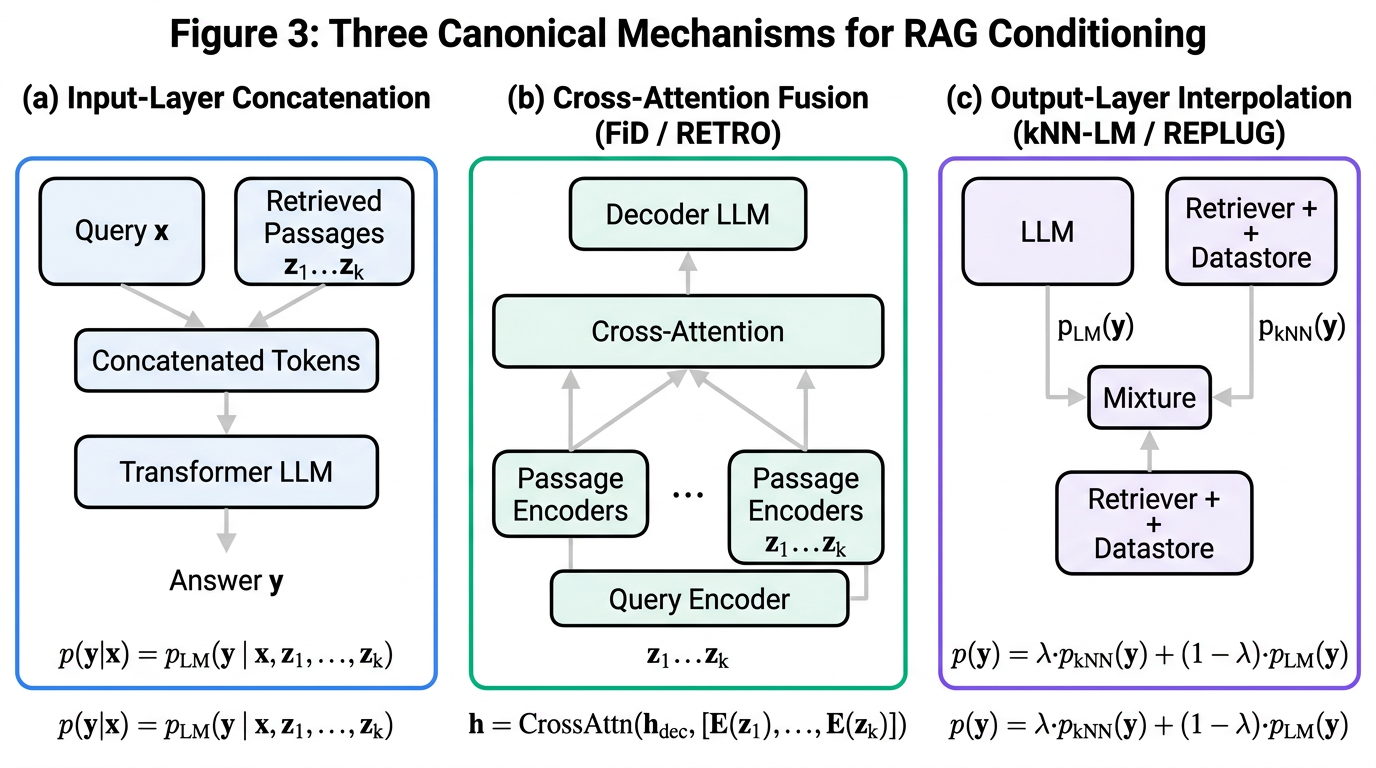
\includegraphics[keepaspectratio,alt={Figure 3. Three canonical algorithmic mechanisms for RAG conditioning}]{./figures/Retrieval-Augmented-Generation-for-Large-Language-Models__fig_mechanisms.png}}
\caption{Figure 3. Three canonical algorithmic mechanisms for RAG conditioning}
\end{figure}

Whereas Section 4 focused on the retrieval pipeline, this section turns to how retrieved evidence is consumed by the generator. This section reviews three canonical conditioning families plus adaptive routing, organized as six subsections that close with a comparative table. The retrieval stage delivers a set \(Z = \{z_1, \dots, z_k\}\) of candidate passages. The generation stage decides what to do with them. Three architectural families have crystallized. First is Fusion-in-Decoder (FiD) and encoder-side concatenation. Second is chunked cross-attention and decoder-side mixing, exemplified by RETRO. Third is black-box conditioning via output-distribution interpolation, exemplified by REPLUG and kNN-LM. Figure 3 contrasts the three. We develop each in detail, with attention to parameter counts, computational complexity, and observed performance trade-offs.

Representative methods include: RAG-Sequence and RAG-Token (Lewis et al., 2020, joint marginalization with per-sequence vs.~per-token mixture), FiD (Izacard \& Grave, 2021, encoder-side independent encoding plus decoder fusion), KG-FiD (Yu et al., 2022, KG-aware passage selection on top of FiD), RETRO (Borgeaud et al., 2022, chunked cross-attention against 2T frozen-BERT tokens), RETRO++ (NVIDIA, 2023, bidirectional retrieval extension of RETRO), Atlas (Izacard et al., 2023, joint Contriever + FiD-T5 with periodic index refresh), REPLUG (Shi et al., 2024, output-distribution ensemble across \(k\) retrieved prompts with LM-supervised retriever tuning), kNN-LM (Khandelwal et al., 2020, token-level interpolation with \(k\)-nearest contexts), In-Context RAG (Ram et al., 2023, frozen-LLM prompt prepend), RA-DIT (Lin et al., 2024, retrieval-augmented dual instruction tuning), InstructRetro (Wang et al., 2024, retrieval-aware pretraining followed by instruction tuning), Self-RAG (Asai et al., 2024, reflection-token policy), FLARE (Jiang et al., 2023, confidence-gated active retrieval), IRCoT (Trivedi et al., 2023, iterative retrieval interleaved with chain-of-thought), Self-Ask (Press et al., 2023, sub-question elicitation), Iter-RetGen (Shao et al., 2023, iterative retrieve-generate synergy), Adaptive-RAG (Jeong et al., 2024, complexity-classifier routing), DRAGIN (Su et al., 2024, dynamic information-need detection), and EnergyRoute (Jang et al., 2026, energy-based gating of retrieval). Each system maps onto exactly one of the three architectural families plus an orthogonal adaptive-routing axis. In summary, the design choice among these families is not aesthetic; each fits a different operational profile, as the comparison table in §5.6 makes precise.

\subsection{Fusion-in-Decoder (FiD) and Encoder-Side Concatenation}\label{fusion-in-decoder-fid-and-encoder-side-concatenation}

Fusion-in-Decoder (FiD) is the architecture of choice when the generator is an encoder-decoder model such as T5 or BART. Introduced by Gautier Izacard and Edouard Grave (EACL 2021), FiD encodes each \((q, z_i)\) pair \emph{independently} with the encoder, concatenates the resulting hidden states \([h_1; h_2; \dots; h_k]\) into a single sequence of length \(\sum_i |h_i|\), and passes the concatenated sequence to the decoder. Independence of the encoder passes is critical: it avoids the quadratic cost of attending across all \((q, z_i)\) pairs jointly, reduces encoder cost from \(O(k^2 L^2)\) to \(O(k L^2)\), and parallelizes trivially across the \(k\) retrieved documents. The decoder, which is the only component that needs to attend across all passages, sees the union of encoder outputs and is therefore able to fuse evidence at the level of individual tokens.

FiD's empirical impact was substantial. FiD-base (220M params) reached 48.2 EM on Natural Questions and 64.7 EM on TriviaQA at \(k=100\) --- outperforming the Lewis et al.~RAG-Token model by 4 EM at NQ. FiD-large (770M) raised these to 51.4 NQ and 67.6 TriviaQA. The crucial finding was that performance kept improving as \(k\) grew from 1 to 100, suggesting that the decoder learns to ignore irrelevant passages and that more retrieval is monotonically better in this architecture. \emph{KG-FiD} (Donghan Yu et al., ACL 2022) extended FiD with knowledge graph augmentation, and \emph{Modeling Multi-Hop QA as Single Sequence Prediction} (Semih Yavuz et al., ACL 2022) showed that FiD's decoder can natively perform multi-hop reasoning when the retriever surfaces the correct chain of passages.

A practical limitation of FiD is decoder context length. With \(k=100\) passages of 200 tokens each, the encoder hidden states span 20,000 positions; modern decoders such as Llama-3 with FlashAttention or Mistral with sliding-window attention handle this comfortably, but inference cost scales linearly. For decoder-only LLMs (GPT-style), the closest equivalent is \emph{prompt concatenation}: simply append the retrieved passages to the prompt and let the decoder attend over them. This is what In-Context RAG (Ori Ram et al., TACL 2023) does, and what every LangChain pipeline produces by default. The conceptual trade-off is that prompt concatenation forces the decoder to do encoder-style work --- re-encoding the retrieved passages on every query --- but it requires no architectural change to the LLM and works with any frozen API.

\subsection{Chunked Cross-Attention (RETRO) and Decoder-Side Mixing}\label{chunked-cross-attention-retro-and-decoder-side-mixing}

RETRO (Sebastian Borgeaud et al., DeepMind, ICML 2022) is the most ambitious architectural intervention in the RAG literature. Its central object is the \emph{Chunked Cross-Attention (CCA)} layer, which is interleaved with self-attention every other block in a decoder transformer. The input is split into chunks of \(L_{ck} = 64\) tokens. For each chunk, a frozen BERT-base retriever fetches \(k=2\) neighbor chunks from a database of two trillion tokens, each neighbor extended by its 64-token continuation. The CCA layer then attends from the current chunk's hidden states to the concatenated neighbor representations --- but crucially, only neighbors of \emph{previous} chunks are attended to, preserving causality.

The mathematical structure of CCA differs from cross-attention in encoder-decoder transformers in three ways. First, the keys and values come from a \emph{frozen} BERT encoder, not from a trained encoder; this freezes the database semantics and makes the index trainable-free. Second, the attention pattern is chunked: each output chunk only attends to its own retrieved neighbors, not to the entire retrieval set. Third, the layer is added every other transformer block, not at every block, which limits parameter overhead to \$\sim\$25 \% of the original model. RETRO-7.5B with a 2T-token database matched the perplexity of GPT-3-175B on the Pile, demonstrating a striking 25× compute-equivalent compression. The cost of pretraining was substantial --- DeepMind reported the retrieval-aware pretraining of RETRO-7.5B at \(\sim 10^{22}\) FLOPs --- but the resulting model could be served with a comparable inference budget to a 7.5B vanilla LM.

RETRO has been generalized in several directions. \emph{Atlas} (Gautier Izacard et al., JMLR 2023) replaced CCA with FiD-style encoder concatenation, allowing a smaller retriever-aware fine-tuning regime that scales to 11B parameters; Atlas-11B achieved 56 EM on NQ in the few-shot setting. \emph{Wang et al.~(EMNLP 2023)} compared retrieval-aware pretraining versus retrieval-aware fine-tuning at 8B and 43B scales, finding that pretraining-integrated retrieval delivers around 4 perplexity points and 6 EM points on NQ over fine-tuning, and that the gains generalize to MMLU-style closed-book QA. \emph{RETRO++ (NVIDIA, 2023)} added bidirectional retrieval. By 2025 the consensus is that retrieval-aware pretraining is a high-value technique reserved for actors at frontier compute scale (DeepMind, NVIDIA, Meta, Anthropic, OpenAI), but downstream fine-tuning on retrieval-augmented data will remain available to smaller labs.

\subsection{Black-Box Conditioning, kNN-LM, and Output Distribution Ensembling}\label{black-box-conditioning-knn-lm-and-output-distribution-ensembling}

The third family of generation-side techniques does not modify the LLM at all but instead operates on its output distribution. \emph{kNN-LM} (Khandelwal et al., ICLR 2020) interpolates the LM's next-token distribution with a softmax over \(k\)-nearest neighbor tokens drawn from the corpus: \(p(w \mid x) = \lambda \, p_{LM}(w \mid x) + (1 - \lambda) \, p_{kNN}(w \mid x)\). The kNN distribution is computed as \(p_{kNN}(w \mid x) \propto \sum_{(c_i, w_i) \in N(x)} \mathbf{1}[w = w_i] \exp(-d(x, c_i) / T)\), where \(N(x)\) is the set of \(k\)-NN contexts. kNN-LM consistently lowers perplexity on Wikitext-103 by 2--4 points and is particularly effective on rare-word domains. Its cost is the additional \(k\)-NN search per token, which becomes substantial for autoregressive generation but is amortizable with batched indexing.

\emph{REPLUG} (Weijia Shi et al., NAACL 2024) operates at the document level instead of the token level. Given a query \(q\) and top-\(k\) retrieved passages, REPLUG runs \(k\) independent forward passes of the LLM with each \((q, z_i)\) as the prompt and produces \(k\) token distributions \(P_i(w \mid q, z_i)\). These are ensembled with weights \(\lambda_i = \text{softmax}(s_\eta(q, z_i))\) proportional to retriever scores: \(p(w) = \sum_i \lambda_i P_i(w)\). Because the LLM is queried only via its output distribution, REPLUG is strictly black-box: it works with closed-source APIs such as GPT-4 and Claude. The retriever can be tuned to maximize the LLM's likelihood of the gold answer --- REPLUG-LSR (LM-supervised retriever) tunes Contriever using GPT-3's perplexity as the reward signal, yielding a 5 EM gain on NQ and 6 points on TriviaQA over a frozen Contriever. The cost is \(k\) LLM calls per query (versus 1 for FiD-style concatenation), so REPLUG is preferred when \(k\) is small (5--10) and the LLM is closed-source.

\subsection{In-Context RAG, Iterative Retrieval, and Self-Reflection}\label{in-context-rag-iterative-retrieval-and-self-reflection}

The simplest and most widely deployed generation-side strategy is \emph{In-Context RAG} (Ori Ram et al., TACL 2023): retrieve top-\(k\) passages once, prepend them to the prompt with a system instruction such as ``Use the following context to answer the question,'' and call the LLM. Ram et al.~showed that on the Pile, a frozen GPT-3-125M with In-Context RAG matches a 1.3B closed-book GPT-3, demonstrating order-of-magnitude parameter compression at inference. In-Context RAG is the deployment pattern of essentially every LangChain, LlamaIndex, and Haystack tutorial; its weakness is that it commits to a single retrieval call before generation begins.

\emph{Iterative retrieval} generalizes In-Context RAG to multiple rounds. \emph{IRCoT} (Trivedi et al., ACL 2023) interleaves chain-of-thought reasoning steps with new retrievals after each step, achieving 65.8 F1 on HotpotQA versus 47.4 with single-shot retrieval. \emph{Self-Ask} (Press et al., ICLR 2023) elicits sub-questions from the LLM and retrieves for each. \emph{FLARE} (Jiang et al., EMNLP 2023) triggers retrieval whenever the LLM's next-token probability falls below a threshold, allowing on-demand retrieval during generation; FLARE outperforms In-Context RAG by 4--6 points on long-form QA. \emph{DSP} and \emph{DSPy} (Omar Khattab et al., ICLR 2024) provide a declarative framework for compiling such iterative pipelines.

\emph{Self-RAG} (Akari Asai et al., ICLR 2024) is the most fully realized self-reflective approach. The Llama-2-7B / Llama-2-13B base model is fine-tuned to emit four families of \emph{reflection tokens}: \texttt{{[}Retrieve{]}} decides whether to retrieve before continuing, \texttt{{[}IsRel{]}} labels each retrieved passage as Relevant or Irrelevant, \texttt{{[}IsSup{]}} labels each generated segment as Supported, Partially Supported, or Not Supported, and \texttt{{[}IsUse{]}} rates the final answer's utility 1--5. Training data is generated by GPT-4 acting as a critic. Self-RAG-7B achieves 43.5 \% accuracy on PubHealth, 54.9 on ARC-Challenge, and beats Llama-2-13B and ChatGPT on TriviaQA; the critic-token formulation has been imitated by RankCoT (Wu et al., ACL 2025), Self-Reflective RAG (multiple 2025 follow-ups), and the \emph{Trustworthy RAG} tradition surveyed by Bo Ni et al.~(arXiv 2502.06872, 2025).

\subsection{Adaptive and Cost-Aware Generation Routing}\label{adaptive-and-cost-aware-generation-routing}

Not every query benefits from retrieval; for closed-book questions, retrieval introduces noise and latency. \emph{Adaptive-RAG} (Soyeong Jeong et al., NAACL 2024) trains a small classifier to label queries as A) closed-book, B) single-shot retrieval, or C) multi-hop iterative retrieval, dispatching each accordingly. On a mixed test set spanning NQ, TriviaQA, HotpotQA, and 2WikiMultiHopQA, Adaptive-RAG achieves a 35 \% latency reduction at equal accuracy. \emph{Self-DC} (Self-Dynamic-Choice) extends this by allowing the LLM itself to issue the routing decision. \emph{EnergyRoute} (Jang et al., 2026) adds an energy-based uncertainty estimator that gates retrieval by per-query confidence.

\subsection{Comparison and Trade-Offs}\label{comparison-and-trade-offs}

Table below summarizes architectural characteristics. The choice among FiD, RETRO-style CCA, In-Context RAG, and REPLUG is not aesthetic --- each fits a different operational profile.

{\def\LTcaptype{none} % do not increment counter
\begin{longtable}[]{@{}
  >{\raggedright\arraybackslash}p{(\linewidth - 14\tabcolsep) * \real{0.1469}}
  >{\raggedright\arraybackslash}p{(\linewidth - 14\tabcolsep) * \real{0.1412}}
  >{\raggedright\arraybackslash}p{(\linewidth - 14\tabcolsep) * \real{0.0791}}
  >{\raggedright\arraybackslash}p{(\linewidth - 14\tabcolsep) * \real{0.1017}}
  >{\raggedright\arraybackslash}p{(\linewidth - 14\tabcolsep) * \real{0.0904}}
  >{\raggedright\arraybackslash}p{(\linewidth - 14\tabcolsep) * \real{0.1073}}
  >{\raggedright\arraybackslash}p{(\linewidth - 14\tabcolsep) * \real{0.1864}}
  >{\raggedright\arraybackslash}p{(\linewidth - 14\tabcolsep) * \real{0.1469}}@{}}
\toprule\noalign{}
\begin{minipage}[b]{\linewidth}\raggedright
Architecture
\end{minipage} & \begin{minipage}[b]{\linewidth}\raggedright
LLM type
\end{minipage} & \begin{minipage}[b]{\linewidth}\raggedright
k typical
\end{minipage} & \begin{minipage}[b]{\linewidth}\raggedright
Cost/query
\end{minipage} & \begin{minipage}[b]{\linewidth}\raggedright
Trains LLM?
\end{minipage} & \begin{minipage}[b]{\linewidth}\raggedright
Trains retriever?
\end{minipage} & \begin{minipage}[b]{\linewidth}\raggedright
Strength
\end{minipage} & \begin{minipage}[b]{\linewidth}\raggedright
Weakness
\end{minipage} \\
\midrule\noalign{}
\endhead
\bottomrule\noalign{}
\endlastfoot
In-Context RAG & Decoder-only frozen & 3--10 & 1 LLM call & No & No & Plug-and-play, works with any API & k limited by context \\
FiD & Encoder-decoder fine-tune & 10--100 & 1 fwd pass & Yes (T5) & Optional & Scales to large k & Requires fine-tuning \\
RAG-Sequence/Token (Lewis) & Encoder-decoder & 5--20 & 1--k passes & Yes & Yes (joint marg.) & End-to-end gradient & Complex \\
RETRO (CCA) & Decoder + CCA & k=2/chunk & Specialized & Pretraining & No (frozen BERT) & 25× compute compression & Pretraining-only \\
REPLUG & Decoder-only frozen & 5--10 & k LLM calls & No & Yes (LM-supervised) & Black-box, closed APIs & k LLM calls cost \\
Self-RAG & Decoder fine-tune & 0--5 (adaptive) & 1--2 calls & Yes (SFT tokens) & No & Self-critique, citation-aware & Fine-tuning required \\
Adaptive-RAG & Decoder + classifier & Variable & Routed & Yes (classifier) & No & Latency-optimal & Classifier training \\
kNN-LM & Decoder + kNN softmax & k tokens & 1 call + kNN/token & No & No & Token-level integration & Slow autoregressive search \\
\end{longtable}
}

Three observations close this section. First, the trend in 2024--2026 is unmistakably toward \emph{frozen-LLM} generation-side designs (In-Context, REPLUG, RAG-via-prompt), because closed-source API LLMs dominate production. Second, \emph{adaptive retrieval} --- Self-RAG, FLARE, Adaptive-RAG, EnergyRoute --- has become the standard rather than the exception in research code. Third, the boundary between RAG and \emph{agentic} LLM systems is dissolving: when an LLM decides what to retrieve, when to retrieve, and how to verify, the system is best understood as an agent with retrieval as one tool among several. This sets up §6 and §7, which examine advanced and structured RAG, respectively.

\section{Advanced RAG Techniques: Query Rewriting, Reranking, and Self-Reflection}\label{advanced-rag-techniques-query-rewriting-reranking-and-self-reflection}

Building on the generation-side architectures of Section 5, this section turns to the pre- and post-retrieval techniques that uplift any architectural backbone. This section reviews query reformulation, reranking, adaptive triggering, hierarchical retrieval, contextual compression, citation generation, and conversational RAG, organized as seven subsections plus an empirical synthesis. The Naive RAG baseline --- embed, retrieve top-\(k\), prepend, generate --- is a strong starting point. It is consistently improved by a handful of Advanced RAG interventions. The empirical study by Xiaohua Wang et al.~(EMNLP 2024, \emph{Searching for Best Practices in Retrieval-Augmented Generation}) measured each intervention in isolation across three tasks (factual QA, multi-hop QA, and long-form QA). The largest gains come from query rewriting, reranking, and adaptive retrieval triggering. We walk through each technique and quantify its impact.

Representative methods include: Multi-Query Expansion (LangChain MultiQueryRetriever, 2023, \(n\)-paraphrase union retrieval), GAR (Mao et al., 2021, generated hypothetical answer/context/title), HyDE (Gao et al., 2022, zero-shot hypothetical document embedding), Query Rewriting (Ma et al., 2023, RL-trained T5 rewriter), Step-Back Prompting (Zheng et al., 2023, abstract-question reformulation), Sub-Question Decomposition (Self-Ask, 2023, atomic sub-query generation), MS-MARCO MiniLM-L-12 (Reimers \& Gurevych, 2020, 33M-param cross-encoder reranker), BGE-Reranker-large (BAAI, 2023, 560M-param cross-encoder), ColBERTv2 (Santhanam et al., 2022, late-interaction reranker-retriever), PromptReps (Zhuang et al., 2024, LLM-prompted dense+sparse representations), RankGPT (Sun et al., 2023, LLM-as-listwise-reranker), RankZephyr (Pradeep et al., 2023, distilled open-source listwise ranker), RankCoT (Wu et al., 2025, chain-of-thought ranking), HtmlRAG (Tan et al., 2025, HTML-tag-aware retrieval and reranking), FLARE (Jiang et al., 2023, token-confidence-gated retrieval), Self-RAG (Asai et al., 2024, reflection-token policy), Adaptive-RAG (Jeong et al., 2024, complexity-classifier routing), Self-DC (Wang et al., 2024, LLM-internal routing), MultiReflect (Kangur et al., 2025, multimodal self-reflection), RAPTOR (Sarthi et al., 2024, recursive abstractive summary tree), HippoRAG (Gutiérrez et al., 2024, Personalized PageRank over entity-passage graph), LongLLMLingua (Jiang et al., 2024, LLM-perplexity-based prompt compression), RECOMP (Xu et al., 2024, extractive context compressor), and ALCE (Gao et al., 2023, citation-generation benchmark and prompt template). Across these methods, the recurring pattern is that small, composable interventions on either the query side or the post-retrieval side yield additive gains; the empirical synthesis in §6.7 quantifies the additive picture.

\subsection{Query Reformulation, HyDE, and Generation-Augmented Retrieval}\label{query-reformulation-hyde-and-generation-augmented-retrieval}

Real user queries are short, ambiguous, and often phrased differently from the corpus documents. \emph{Query rewriting} uses an auxiliary LLM to transform the user query into a form that better matches the index. The simplest form is \emph{paraphrase expansion}: ask the LLM to generate \(n=3\)--\(5\) paraphrases and take the union of retrieved passages. This is the basis of LangChain's \texttt{MultiQueryRetriever} and LlamaIndex's \texttt{QueryFusionRetriever}. Empirically, a 5-paraphrase expansion lifts NQ Recall@10 by 3--5 points and HotpotQA Recall@10 by 6--8 points.

\emph{Generation-Augmented Retrieval} (GAR; Yuning Mao et al., ACL 2021) is a more principled rewriter. Given a query \(q\), GAR uses a fine-tuned BART model to generate three artifacts: a hypothetical answer, a hypothetical context sentence, and a hypothetical title. These are concatenated to the query for retrieval. GAR raised NQ Recall@5 from 71.5 (DPR alone) to 75.4. \emph{HyDE} (Hypothetical Document Embeddings; Gao et al., 2022) generalizes this to zero-shot retrieval: prompt an LLM to generate a fake passage that \emph{would} answer the question, embed the fake passage, and retrieve. HyDE recovers most of the gains of supervised dense retrievers without any labeled data, making it the default for cold-start RAG over new corpora.

\emph{Query Rewriting} (Xinbei Ma et al., EMNLP 2023) trains a small T5-based rewriter via reinforcement learning, using the retriever's nDCG@10 as the reward signal and the LLM's correctness on the final answer as a downstream signal. The resulting rewriter improves multi-hop questions by 2.4 EM. \emph{Step-Back Prompting} (Zheng et al., 2023) generates a more abstract, ``step-back'' version of the question, which often retrieves better evidence for narrow factoids. \emph{Sub-query decomposition}, used in RAPTOR and Self-Ask, breaks a multi-hop question into atomic sub-queries and retrieves for each.

\subsection{Cross-Encoder Reranking, Late Interaction, and RankCoT}\label{cross-encoder-reranking-late-interaction-and-rankcot}

After first-stage retrieval (typically Recall@100 around 90 \%), a \emph{reranker} re-orders the top-100 to produce the top-\(k\) that the LLM will consume. Cross-encoder rerankers concatenate \((q, z)\) and pass them through a transformer with a single classification head. Classic instances include \texttt{cross-encoder/ms-marco-MiniLM-L-12-v2} (33M params, BEIR nDCG@10 +5 over BM25), \texttt{cross-encoder/ms-marco-electra-base} (110M, BEIR +6.5), and \texttt{BAAI/bge-reranker-large} (560M, BEIR +8). On a query batch of 100 candidates, a cross-encoder reranker adds 30--60 ms of latency on an A100 GPU.

Late-interaction models such as \emph{ColBERTv2} (Keshav Santhanam et al., NAACL 2022) blur the retriever--reranker boundary: their per-token MaxSim score is itself a fine-grained ranker that beats first-stage dense retrievers without an additional cross-encoder pass, achieving BEIR nDCG@10 of 0.49 versus DPR's 0.41. ColBERT-style architectures are increasingly used as one-stage retrievers in production (Vespa, Jina ColBERT). \emph{PromptReps} (Shengyao Zhuang et al., EMNLP 2024) uses a small LLM to generate dense and sparse representations in a single prompt, enabling zero-shot retrieval with no contrastive training.

\emph{RankGPT} (Sun et al., 2023) and \emph{RankZephyr} prompt an LLM to rerank a list of retrieved passages directly: the LLM is asked to output a permutation of identifiers in order of relevance. RankGPT-4 outperforms cross-encoder rerankers by 2--4 nDCG@10 on BEIR and is particularly strong on long-tail entity queries. \emph{RankCoT} (Mingyan Wu et al., ACL 2025) extends this with chain-of-thought reasoning during ranking: the LLM produces a brief justification for each candidate before issuing the final ranking, gaining 2--3 EM on multi-hop QA. The cost is one additional LLM call per query.

\subsection{Self-RAG, FLARE, and Adaptive Retrieval Triggering}\label{self-rag-flare-and-adaptive-retrieval-triggering}

Whether to retrieve at all is itself a decision worth optimizing. \emph{FLARE} (Active Retrieval Augmented Generation; Zhengbao Jiang et al., EMNLP 2023) triggers a new retrieval whenever the LLM's next-token probability for any token in a generated sentence falls below a threshold \(\tau\). The motivating intuition is that low-probability tokens often correspond to factual claims that the LLM is uncertain about; FLARE retrieves at exactly those points and re-runs generation with the new evidence. On long-form benchmarks (StrategyQA, ASQA), FLARE outperforms In-Context RAG by 4--6 F1 points.

\emph{Self-RAG} (Akari Asai et al., ICLR 2024) integrates retrieval triggering into the generation policy. The LLM is fine-tuned with reflection tokens --- \texttt{{[}Retrieve{]}}, \texttt{{[}NoRetrieve{]}}, \texttt{{[}IsRel:Relevant/Irrelevant{]}}, \texttt{{[}IsSup:Fully/Partially/NotSupported{]}}, \texttt{{[}IsUse:1..5{]}} --- and learns to decide on its own when retrieval is necessary. Empirically, Self-RAG-7B retrieves on roughly 60 \% of TriviaQA queries and skips retrieval on the rest, yielding a 30 \% latency reduction at improved accuracy. The reflection tokens additionally serve as a calibration signal for downstream verification.

\emph{Adaptive-RAG} (Soyeong Jeong et al., NAACL 2024) trains a small classifier to label each query as A) closed-book, B) single-shot retrieval, or C) multi-hop iterative retrieval. The classifier --- a 110M-param BERT --- adds \(<10\) ms of latency per query but cuts overall pipeline cost by 35 \% on a mixed test set. \emph{Self-Reflective RAG} approaches such as MultiReflect (Kangur et al., 2025) extend the idea to multimodal fact-checking, and \emph{Self-DC} (Wang et al., 2024) lets the LLM itself emit the routing token without an external classifier.

\subsection{Hierarchical and Compressed Retrieval: RAPTOR, Tree-Organized Retrieval}\label{hierarchical-and-compressed-retrieval-raptor-tree-organized-retrieval}

For long documents and multi-document corpora, flat chunking discards hierarchical structure. \emph{RAPTOR} (Parth Sarthi, Salman Abdullah, Aditi Tuli, Shubh Khanna, Anna Goldie, Christopher D. Manning; ICLR 2024) builds a \emph{recursive abstractive summary tree} over the corpus: leaf nodes are 200-token chunks, internal nodes are LLM-generated summaries of their children, formed by recursively clustering with Gaussian Mixtures and summarizing each cluster. At query time, RAPTOR retrieves nodes from any tree level, allowing both fine-grained (``which year did X happen?'') and high-level (``what is this document about?'') questions to surface relevant context. RAPTOR + GPT-4 achieves +20 \% over flat chunking on the QuALITY benchmark and is now standard in LlamaIndex's \texttt{HierarchicalNodeParser}. \emph{Tree-organized self-reflective retrieval} in TCM-QA (Liu et al., 2026) extends the idea to traditional Chinese medicine.

\subsection{Contextual Compression, Citation Generation, and Faithfulness}\label{contextual-compression-citation-generation-and-faithfulness}

Retrieved passages are often longer than necessary. \emph{Contextual compression} --- surveyed by Sourav Verma (arXiv 2409.13385, 2024) --- uses an LLM-based extractor to keep only the spans relevant to the query, achieving 4--8× compression with \(<2\) EM loss. \emph{LongLLMLingua} (Jiang et al., 2024) compresses prompts at the token level using an LLM-derived perplexity score, and \emph{RECOMP} (Xu et al., 2024) trains a dedicated extractive compressor.

\emph{Enabling Large Language Models to Generate Text with Citations} (Tianyu Gao et al., EMNLP 2023) introduced the ALCE benchmark for citation generation and showed that prompting the LLM to cite specific passages by ID improves attribution accuracy from 35 \% to 70 \%. \emph{Citation faithfulness} --- that every claim in the answer is supported by at least one cited passage --- has become a core evaluation axis in RAGAS, ARES, and TruLens. \emph{RankCoT} (Wu et al., ACL 2025) incorporates citation reasoning into the ranking step.

\subsection{Conversational and Multi-Turn RAG}\label{conversational-and-multi-turn-rag}

Real applications are conversational, and conversational RAG must handle pronoun resolution, topic drift, and context carry-over. \emph{Contextualized Query Embeddings for Conversational Search} (Sheng-Chieh Lin et al., EMNLP 2021) trains a query encoder that takes the entire dialog history into account, lifting MRR@10 by 8 points on the CAsT 2020 benchmark over single-turn DPR. \emph{Internet-Augmented Dialog} (Mojtaba Komeili, Kurt Shuster, Jason Weston; ACL 2022) introduced live-search RAG for dialog and showed substantial gains in factual currency over BlenderBot 2. The 2025 \emph{MTRAG benchmark} (Yannis Katsis et al., Qeios 2025) is the first widely cited multi-turn RAG evaluation: it found that even strong single-turn RAG systems lose 15--25 \% of accuracy in multi-turn settings, with the largest drops occurring when the user refers back to entities mentioned several turns earlier.

{\def\LTcaptype{none} % do not increment counter
\begin{longtable}[]{@{}
  >{\raggedright\arraybackslash}p{(\linewidth - 6\tabcolsep) * \real{0.1875}}
  >{\raggedright\arraybackslash}p{(\linewidth - 6\tabcolsep) * \real{0.2578}}
  >{\raggedright\arraybackslash}p{(\linewidth - 6\tabcolsep) * \real{0.3594}}
  >{\raggedright\arraybackslash}p{(\linewidth - 6\tabcolsep) * \real{0.1953}}@{}}
\toprule\noalign{}
\begin{minipage}[b]{\linewidth}\raggedright
Technique
\end{minipage} & \begin{minipage}[b]{\linewidth}\raggedright
What is added
\end{minipage} & \begin{minipage}[b]{\linewidth}\raggedright
Typical gain
\end{minipage} & \begin{minipage}[b]{\linewidth}\raggedright
Cost added
\end{minipage} \\
\midrule\noalign{}
\endhead
\bottomrule\noalign{}
\endlastfoot
Multi-query expansion & n=3--5 paraphrases & +3--5 NQ R@10, +6--8 HotpotQA R@10 & n× retriever calls \\
HyDE & Hypothetical doc & +5--10 R@10 zero-shot & 1 LLM call \\
GAR & Hypothetical answer/context/title & +4 NQ R@5 & 1 LLM call \\
Query Rewriting (Ma '23) & RL-trained rewriter & +2.4 EM multi-hop & 1 small LLM call \\
Step-Back Prompting & Abstract reformulation & +3 EM narrow factoids & 1 LLM call \\
Cross-encoder rerank & MiniLM/BGE reranker & +5--8 BEIR nDCG@10 & 30--60 ms/query \\
RankGPT & LLM as reranker & +2--4 nDCG@10 over CE & 1 LLM call \\
RankCoT & CoT during ranking & +2--3 EM multi-hop & 1 LLM call \\
FLARE active retrieval & Confidence-gated re-retrieve & +4--6 long-form F1 & Variable (usually +1 LLM) \\
Self-RAG & Reflection tokens & Llama-2-7B beats Llama-13B/ChatGPT on TriviaQA & SFT cost; --30 \% runtime \\
Adaptive-RAG & Complexity classifier & --35 \% latency at equal accuracy & 110M BERT \\
RAPTOR & Tree-organized summary index & +20 \% QuALITY over flat chunks & \textasciitilde5× indexing cost \\
Contextual compression & LLM-extractive shortening & 4--8× shorter, \textless2 EM loss & 1 small LLM call \\
ALCE citation & Per-passage citation & Attribution 35→70 \% & None \\
MTRAG / multi-turn & Dialog-aware retriever & Recovers 15--25 \% multi-turn drop & Dialog-context encoder \\
\end{longtable}
}

\subsection{Searching for Best Practices: Empirical Synthesis}\label{searching-for-best-practices-empirical-synthesis}

Wang et al.~(EMNLP 2024) conducted the largest single-paper empirical study to date. Their take-aways: (1) chunk size 256 tokens with 10 \% overlap is the robust default; (2) BGE-large-en (or BGE-M3 multilingual) is the dominant open-weight embedder; (3) cross-encoder reranking on top of dense retrieval gains 4 EM on average and is worth its 30--60 ms cost; (4) k=5--10 retrieved passages is the sweet spot for 7B--13B LLMs, while k=20--50 is preferred for FiD-style architectures; (5) multi-query expansion costs little and delivers reliable gains; (6) HyDE excels in zero-shot domains; (7) Self-RAG / Adaptive-RAG style routing is justified when query mix spans multiple complexity levels.

The 2025 \emph{Pandora's Box or Aladdin's Lamp} analysis (Jinyang Wu et al., ACL 2025) re-examined RAG noise robustness and found that \emph{some} irrelevant passages in \(Z\) can actually act as helpful regularizers, encouraging the LLM to ignore unsupported context. This nuance --- that retrieval noise is not strictly harmful --- has motivated new training regimes such as \emph{Adversarial Adaptive Training} (Feiteng Fang et al., ACL 2024) which deliberately injects irrelevant passages during fine-tuning. The trajectory of advanced RAG research is increasingly statistical: techniques are evaluated not on whether they always help but on the conditions under which they help, anticipated by the survey of Aoran Gan et al.~(arXiv 2504.14891, 2025) on RAG evaluation.

\section{Structured and Multimodal RAG (GraphRAG, HybridRAG, Vision-RAG)}\label{structured-and-multimodal-rag-graphrag-hybridrag-vision-rag}

Whereas Section 6 focused on advanced techniques over flat text, this section turns to RAG over structured and multimodal corpora. This section reviews graph-augmented RAG, hybrid vector-plus-symbolic RAG, vision-language RAG, code and tabular RAG, and long-document multimodal RAG, organized as six subsections plus a comparative table. The 2024--2026 frontier of RAG has expanded from flat text indexes to \emph{structured} corpora and to \emph{multimodal} corpora. Structured corpora include knowledge graphs, tables, and code ASTs. Multimodal corpora include images, audio, video, and scientific figures. Two surveys mark the entry of this subfield into the mainstream: the \emph{Graph Retrieval-Augmented Generation: A Survey} of Boci Peng, Yun Zhu, Yongchao Liu et al.~(arXiv 2408.08921, 2024) and \emph{A Survey of Graph Retrieval-Augmented Generation for Customized Large Language Models} of Qinggang Zhang et al.~(arXiv 2501.13958, 2025). The defining shift is that retrieval is no longer only over flat passages. Retrieval now operates over typed entities, relations, and structured records. The LLM is asked to integrate evidence with topology.

Representative methods include: GraphRAG (Edge et al., Microsoft, 2024, LLM-extracted KG plus hierarchical Leiden community summarization), LightRAG (Guo et al., 2025, simplified two-level graph retrieval), HybridRAG (Sarmah et al., 2024, vector + KG fusion for finance), HippoRAG (Gutiérrez et al., 2024, Personalized PageRank over entity-passage graph), G-Retriever (He et al., 2024, Steiner-tree subgraph extraction), KG-RAG / SPOKE (Soman et al., 2024, biomedical KG with literature linkage), KG-FiD (Yu et al., 2022, KG-aware FiD passage selection), JAKET (Yu et al., 2022, joint entity-text pretraining), TrumorGPT (Hang et al., 2025, graph-based fact-checking), KG-augmented executable CoT (Chen et al., 2026, KG paths for symbolic mathematical coding), Document GraphRAG (Knollmeyer et al., 2025, manufacturing-domain Q\&A), Hybrid Multi-Agent GraphRAG (Papageorgiou et al., 2025, e-government layer), RA-CM3 (Yasunaga et al., 2023, retrieval-augmented multimodal pretraining), MAGIC (Su et al., 2022, training-free CLIP-based captioning), Retrieval-Augmented Image Captioning (Ramos et al., 2023, CLIP-retrieved nearest captions), Chest X-Ray RAG (Ranjit et al., 2023, anatomy-aligned image-report retrieval), VLM-RAG-Melanoma (Moon \& Hong, 2025, dermatology VLM retrieval), Augmenting Orbital Debris Identification (Roll et al., 2025, Neo4j graph plus LLaVA), RepoCoder (Zhang et al., 2023, iterative repository-local code retrieval), DocPrompting (Zhou et al., 2023, retrieved API-doc snippets), kNN-LM-Code (token-level code retrieval), UniK-QA (Oğuz et al., 2022, table-flattened DPR), MT-RAIG (Seo et al., 2025, multi-table insight generation), IoT-LLM (An et al., 2026, sensor-time-series augmented LLM), PodGPT (Jia et al., 2025, podcast-transcribed audio retrieval), and RadOncRAG (Thaker et al., 2025, radiation oncology with figure understanding). In summary, the structured/multimodal RAG landscape is heterogeneous in modalities but converges on a shared problem statement: retrieval scoring must combine vector similarity with topology, structure, or modality alignment, and the LLM must learn to consume the resulting non-textual evidence.

\subsection{Graph and Knowledge-Graph Augmentation}\label{graph-and-knowledge-graph-augmentation}

\emph{GraphRAG} --- popularized by the Microsoft Research system of Edge et al.~(arXiv 2404.16130, 2024) --- builds a knowledge graph over the corpus by LLM-extracted entity-relation triples, then applies hierarchical community detection (Leiden algorithm) and per-community LLM summarization. At query time, GraphRAG retrieves a community summary appropriate to the query's scope and asks the LLM to answer using it. The headline result on the \emph{Sufficient Coverage} metric was a 70--80 \% relative gain over flat vector RAG for \emph{query-focused summarization} --- questions like ``what are the main themes of these reports?'' that flat retrievers cannot answer because no single passage contains the answer.

\emph{Local} and \emph{global} retrieval modes coexist in GraphRAG. Local mode retrieves the entities most relevant to the query plus their ego-network; global mode retrieves community summaries at a chosen level of the hierarchy. \emph{DRIFT} search interleaves both. \emph{KG-RAG} (Soman et al., 2024) for biomedical Q\&A uses SPOKE, a 3.4M-node biomedical KG, and connects nodes to literature passages, lifting MedQA accuracy by 4 points. \emph{G-Retriever} (He et al., NeurIPS 2024) frames KG retrieval as a Steiner Tree problem: find the minimum-cost subgraph connecting query-relevant entities. \emph{HippoRAG} (Gutiérrez et al., NeurIPS 2024) uses Personalized PageRank over an entity-passage graph and gains 12 EM on multi-hop benchmarks.

\emph{JAKET} (Donghan Yu et al., AAAI 2022) jointly pre-trains language models with knowledge graphs by injecting entity embeddings into the transformer; it is a precursor to LLM+KG fusion. \emph{KG-FiD} (Donghan Yu et al., ACL 2022) extends FiD with KG-aware passage selection. \emph{Trumor}GPT (Hang et al., IEEE TAI 2025) applies graph-based retrieval to fact-checking. The KG-augmented executable CoT for mathematical coding (Chen et al., Neural Networks 2026) demonstrates KG-RAG for symbolic reasoning. The \emph{Survey of Graph RAG for Customized LLMs} (Zhang et al., 2025) and \emph{Graph RAG with Graphs} (Han et al., 2025) classify this subfield along three axes: graph topology (homogeneous, heterogeneous, dynamic), retrieval mechanism (subgraph, path, embedding), and integration (text-linearization, GNN encoding, prompt template).

\subsection{Hybrid Vector + Symbolic Retrieval (HybridRAG)}\label{hybrid-vector-symbolic-retrieval-hybridrag}

A pragmatic compromise is \emph{HybridRAG} (Bhaskarjit Sarmah, Dhagash Mehta, Benika Hall et al., ACM ICAIF 2024), which fuses a knowledge graph retriever with a vector retriever and lets the LLM see both. On the FinanceBench earnings-calls benchmark, HybridRAG cut answer error rate from 26 \% (vector-only) and 31 \% (KG-only) to 14 \%. The pattern works because vector retrieval excels on paraphrased phrases and unstructured context while KG retrieval excels on entity disambiguation and relation chains; the two modalities complement.

\emph{Document GraphRAG} (Knollmeyer et al., Electronics 2025) extends HybridRAG to manufacturing-domain Q\&A. \emph{Hybrid Multi-Agent GraphRAG} (Papageorgiou et al., 2025) layers an agent on top of the hybrid retriever for e-government applications. \emph{KG-augmented executable Chain-of-Thought} (Xingyu Chen et al., Neural Networks 2026) integrates symbolic KG paths with executable code and is particularly effective for mathematical coding problems.

\subsection{Vision-Language and Multimodal Retrieval Pipelines}\label{vision-language-and-multimodal-retrieval-pipelines}

Multimodal RAG operates over a corpus of images, image-text pairs, or videos. The retriever is typically a CLIP-style joint vision-language encoder. \emph{Retrieval-Augmented Image Captioning} (Rita Ramos, Desmond Elliott, Bruno Martins; EACL 2023) retrieves nearest-neighbor captions for an input image and conditions a small captioning model on them; this beats much larger captioning models that lack retrieval, particularly on rare object categories. \emph{MAGIC} (Su et al., 2022) does training-free image captioning by retrieving and re-ranking with CLIP. \emph{RA-CM3} (Yasunaga et al., 2023) adds retrieval to CM3 for retrieval-augmented multimodal pretraining.

In medical imaging, \emph{Retrieval-Augmented Chest X-Ray Report Generation} (Mercy Ranjit et al., arXiv 2305.03660, 2023) retrieves anatomy-aligned image-report pairs and conditions GPT-4 to write the report, lifting CheXbert F1 by 4 points over GPT-4 alone. \emph{ChatTogoVar} (Mitsuhashi et al., 2026) retrieves over a genomic variant database. \emph{MedDiscover} (Patel et al., 2026) builds a domain-specific retriever for metabolomics. \emph{VLM-RAG} for melanoma (Moon \& Hong, AVSS 2025) integrates vision and clinical-text retrieval. The 2024 \emph{Multimodal RAG Evaluation Benchmark} (Sun et al., VTC Spring 2024) is the first dedicated benchmark for the modality.

\emph{Visual GraphRAG} applies graph augmentation to vision: \emph{Augmenting Orbital Debris Identification with Neo4j-Enabled Graph-Based Retrieval-Augmented Generation for Multimodal Large Language Models} (Daniel S. Roll et al., Sensors 2025) builds a Neo4j graph of debris properties and retrieves both image embeddings and graph context for an LLaVA-based MLLM. \emph{Long-text caption generation for surgical images} (Liu et al., 2026) constructs a concept-aware retriever over surgical literature.

\subsection{Code, Tabular, and Time-Series RAG}\label{code-tabular-and-time-series-rag}

\emph{Code RAG} --- retrieving code snippets, documentation, or repository context --- has become standard in production code assistants. GitHub Copilot Chat retrieves repository-local context via a custom dense retriever; \emph{RepoCoder} (Zhang et al., 2023) applies iterative retrieval over code repositories; \emph{ReAcc} and \emph{kNN-LM-Code} propagate the kNN-LM idea to code. \emph{DocPrompting} (Zhou et al., 2023) retrieves API documentation snippets to improve generation of unfamiliar API calls.

\emph{Tabular RAG} targets corpora of structured tables. \emph{UniK-QA} (Barlas Oğuz et al., NAACL 2022) flattens tables into text and retrieves via DPR; \emph{Open-WikiTable} and \emph{FetaQA} are common benchmarks. \emph{MT-RAIG} (Seo et al., ACL 2025) is a multi-table retrieval-augmented insight-generation benchmark, addressing queries that require combining several tables. For time-series, \emph{IoT-LLM} (An et al., Patterns 2026) augments LLM reasoning with retrieval over real-world sensor data.

\subsection{Conversational and Long-Document Multimodal RAG}\label{conversational-and-long-document-multimodal-rag}

Long-document multimodal RAG combines retrieval over text, images, and figures within scientific PDFs and technical manuals. \emph{Scientific Multimodal RAG} using vision-language models retrieves figure embeddings alongside text. \emph{RadOncRAG} (Thaker et al., JCO Clinical Cancer Informatics 2025) retrieves over radiation oncology literature with figure understanding and clinical decision support. \emph{PodGPT} (Jia et al., npj Biomedical Innovations 2025) constructs an audio-augmented retrieval-augmented LLM by transcribing scientific podcasts and indexing the transcripts with topic tags for downstream Q\&A.

\subsection{Comparative Profile of Structured/Multimodal RAG Variants}\label{comparative-profile-of-structuredmultimodal-rag-variants}

{\def\LTcaptype{none} % do not increment counter
\begin{longtable}[]{@{}
  >{\raggedright\arraybackslash}p{(\linewidth - 10\tabcolsep) * \real{0.2705}}
  >{\raggedright\arraybackslash}p{(\linewidth - 10\tabcolsep) * \real{0.2131}}
  >{\raggedright\arraybackslash}p{(\linewidth - 10\tabcolsep) * \real{0.1721}}
  >{\raggedright\arraybackslash}p{(\linewidth - 10\tabcolsep) * \real{0.1230}}
  >{\raggedright\arraybackslash}p{(\linewidth - 10\tabcolsep) * \real{0.1475}}
  >{\raggedright\arraybackslash}p{(\linewidth - 10\tabcolsep) * \real{0.0738}}@{}}
\toprule\noalign{}
\begin{minipage}[b]{\linewidth}\raggedright
System / paradigm
\end{minipage} & \begin{minipage}[b]{\linewidth}\raggedright
Modalities
\end{minipage} & \begin{minipage}[b]{\linewidth}\raggedright
Retriever
\end{minipage} & \begin{minipage}[b]{\linewidth}\raggedright
Generator
\end{minipage} & \begin{minipage}[b]{\linewidth}\raggedright
Domain
\end{minipage} & \begin{minipage}[b]{\linewidth}\raggedright
Year
\end{minipage} \\
\midrule\noalign{}
\endhead
\bottomrule\noalign{}
\endlastfoot
GraphRAG (Microsoft) & Text + KG (LLM-extracted) & Community summary & GPT-4 & Open / news & 2024 \\
HybridRAG & Text + KG & DPR + KG-walk & GPT-4 & Finance / earnings & 2024 \\
HippoRAG & Text + entity graph & Personalized PageRank & Llama-2 & Multi-hop QA & 2024 \\
G-Retriever & Text-attributed graph & Steiner-tree subgraph & GraphLLM & Web / KG QA & 2024 \\
KG-RAG / SPOKE & Biomedical KG + text & KG walk + DPR & GPT-4 & Medicine & 2024 \\
RA-CM3 / MAGIC & Image + caption & CLIP & CM3 / GPT-2 & Captioning & 2023 \\
Retrieval-Aug Image Captioning & Image + caption & CLIP & small captioner & General captioning & 2023 EACL \\
Chest X-Ray RAG & Image + report & CLIP-Med & GPT-4 & Radiology & 2023 \\
MedDiscover & Biomed KG + lit. & Custom bio-embedder & LLM & Metabolomics & 2026 \\
ChatTogoVar & Genomic DB + LLM & Variant retriever & LLM & Human genomics & 2026 \\
VLM-Melanoma RAG & Skin image + lit. & CLIP + DPR & VLM & Dermatology & 2025 AVSS \\
Augmenting Orbital Debris (Neo4j) & Image + property graph & Graph + image emb. & LLaVA & Aerospace & 2025 \\
RepoCoder & Code & Code-DPR & StarCoder & Code completion & 2023 \\
MT-RAIG & Multiple tables & Table-aware retriever & LLM & Tabular insight & 2025 \\
IoT-LLM & Sensor time-series + text & Custom hybrid & LLM & IoT reasoning & 2026 \\
PodGPT & Audio (transcribed) + text & DPR over transcripts & LLM & Edu / research & 2025 \\
\end{longtable}
}

\subsection{Common Themes and Open Challenges}\label{common-themes-and-open-challenges}

Three themes recur across structured and multimodal RAG. First, \emph{retrieval is heterogeneous}: scoring functions must combine vector similarity with graph topology, table structure, or modality alignment, and combining them is non-trivial. Reciprocal rank fusion is widely used but ad-hoc. Second, \emph{the LLM must be taught to use structure}: simply concatenating triples or table rows often fails because the LLM defaults to surface form. KG-FiD, HippoRAG, and GraphRAG all use specialized prompt templates or auxiliary GNNs to encode topology. Third, \emph{evaluation is under-developed}: most graph-RAG and multimodal-RAG papers introduce custom test sets, and benchmark fragmentation slows comparison. The MEMERAG (Cruz Blandón et al., ACL 2025) and Multimodal RAG Eval Benchmark (Sun et al., 2024) initiatives partially address this for multilingual and multimodal RAG respectively, while the \emph{Graph RAG for Customized LLMs} survey (Zhang et al., 2025) calls for a unified benchmark.

The trajectory points toward \emph{unified retrieval-augmented multimodal LLMs}: a single model that can retrieve over text, code, KG, table, image, and time-series simultaneously, exemplified by \emph{Materials Dual-Source Knowledge Retrieval-Augmented Generation} (Takahara et al., JCIM 2025) for photocatalysts and the multi-source \emph{MetaSepsisKnowHub} (Zhang et al., JMIR 2025) for sepsis management. The deeper challenge is that the embedding-space alignment across modalities is brittle, and embedding-time-and-modality drift will be a research focus through 2026. The next section turns to the most empirically critical aspect of any RAG system: how it is evaluated.

\section{Datasets, Benchmarks, and Evaluation Methodology}\label{datasets-benchmarks-and-evaluation-methodology}

\begin{figure}
\centering
\pandocbounded{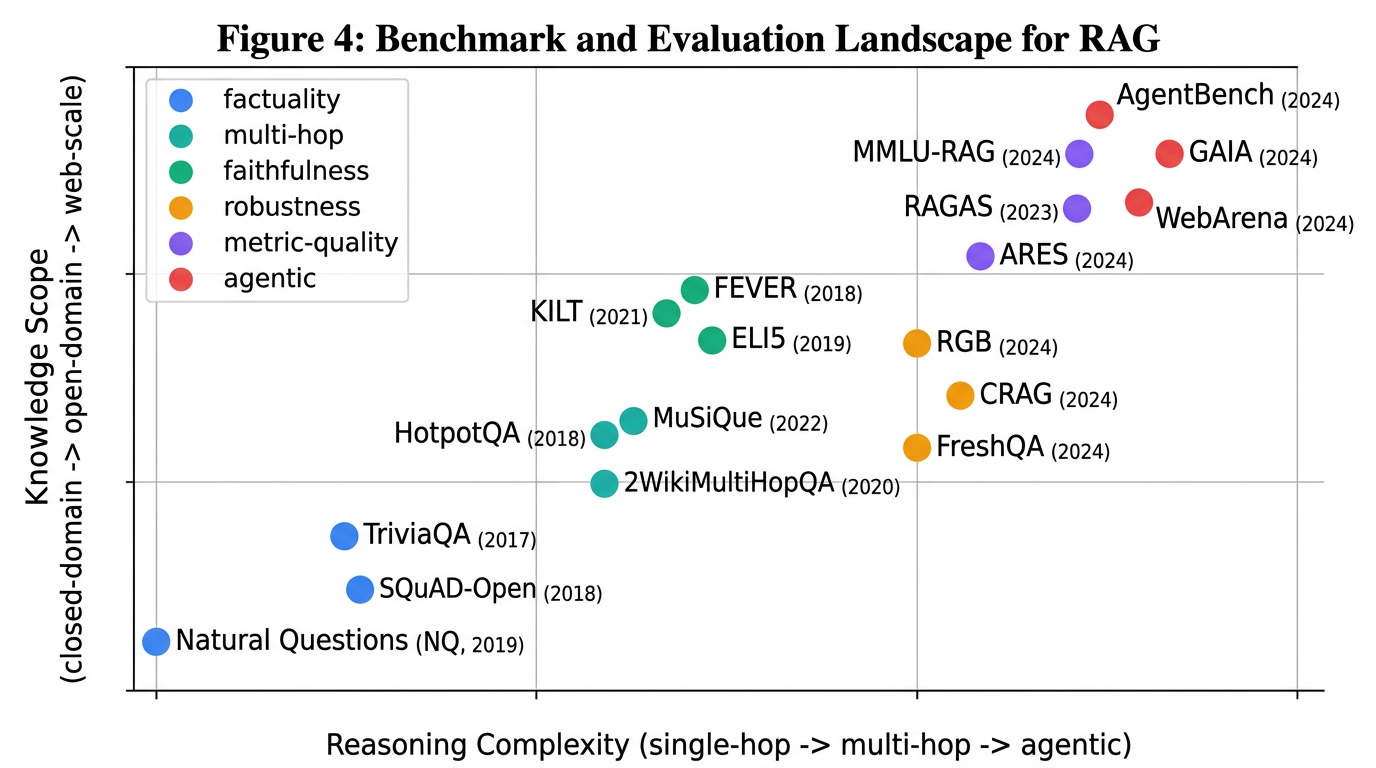
\includegraphics[keepaspectratio,alt={Figure 4. Benchmark and evaluation landscape for RAG over LLMs}]{./figures/Retrieval-Augmented-Generation-for-Large-Language-Models__fig_benchmarks.png}}
\caption{Figure 4. Benchmark and evaluation landscape for RAG over LLMs}
\end{figure}

Whereas Section 7 surveyed structured and multimodal RAG variants, this section turns to how all RAG systems are evaluated. This section reviews knowledge-intensive benchmarks, RAG-specific benchmarks, automatic evaluation frameworks, metrics, compute-cost profiles, and limitations, organized as six subsections. The credibility of any RAG advance depends on the rigor of its evaluation. Two surveys provide a common reference. The first is the \emph{Retrieval Augmented Generation Evaluation in the Era of LLMs: A Comprehensive Survey} by Aoran Gan, Hao Yu, Kai Zhang et al.~(arXiv 2504.14891, 2025). The second is the \emph{Benchmarking of RAG: A Comprehensive Systematic Literature Review} by Simon Knollmeyer et al.~(KMIS 2024). We compile the datasets used to train and probe RAG systems, the dedicated RAG benchmarks introduced since 2024, the metrics that have stabilized into community standards, and the automatic evaluation frameworks (RAGAS, ARES, TruLens) that now dominate practical evaluation.

Representative datasets and benchmarks include: Natural Questions (Kwiatkowski et al., 2019, 307K Google-search QA pairs over Wikipedia), TriviaQA (Joshi et al., 2017, 95K trivia QA), HotpotQA (Yang et al., 2018, 113K multi-hop questions), 2WikiMultiHopQA (193K multi-hop with reasoning paths), MuSiQue (compositional multi-hop), Bamboogle (multi-hop adversarial), MultiHop-RAG (Tang \& Yang, 2024, financial-news multi-hop), PopQA (Mallen et al., 2023, 14K long-tail entity QA), ASQA (long-form ambiguous), ELI5 (long-form explainer), FEVER (Thorne et al., 2018, 185K fact-verification), KILT (Petroni et al., 2021, eleven-task meta-benchmark), BEIR (Thakur et al., 2021, 18-dataset retriever benchmark), MS MARCO (Bajaj et al., 2018, 8.8M passage retrieval corpus), TREC-COVID (pandemic retrieval), TREC-CAsT (conversational retrieval), MIRACL (Zhang et al., 2023, 18-language retrieval), Mr.~TyDi (Zhang et al., 2021, 11-language retrieval), XOR-TyDi (cross-lingual open-domain QA), RGB (Chen et al., 2024, four-axis robustness), RAGTruth (Niu et al., 2024, 18K hallucination-annotated responses), MTRAG (Katsis et al., 2025, multi-turn RAG), MIRAGE (Park et al., 2025, metric-comparison benchmark), MedRAG/MIRAGE-Med (Xiong et al., 2024, five-task medical RAG), ChronoQA (Chen et al., 2025, Chinese temporal RAG), CRUD-RAG (Lyu et al., 2024, Create-Read-Update-Delete), DomainRAG (Wang et al., 2024, six-domain Chinese), MEMERAG (Cruz Blandón et al., 2025, multilingual meta-evaluation), MT-RAIG (Seo et al., 2025, multi-table), IRSC (Lin et al., 2025, semantic comprehension), MeteoRAG (climate, 2025), CyberMetric (Tihanyi et al., 2024, cybersecurity), RAGCare-QA (Dobreva et al., 2025, 420 medical theory questions), ALCE (Gao et al., 2023, 953 long-form citation queries), FaithEval (Ming et al., 2024, counterfactual faithfulness), and FreshQA (Vu et al., 2023, freshness-sensitive QA). Representative evaluation frameworks include: RAGAS (Es et al., 2024, four LLM-judge metrics), ARES (Saad-Falcon et al., 2024, synthetic-question PPI framework), TruLens (TruEra, programmable harness with lineage), EvalLM (calibration-corrected LLM judge), PromptBench (extensible prompt evaluation), and RAGGED (RAG-specific gold-data construction). Crucially, the field has converged on RAGAS as a de-facto industrial standard, while RGB and MultiHop-RAG dominate research-paper reporting.

\subsection{Knowledge-Intensive Benchmarks: NQ, TriviaQA, HotpotQA, FEVER, KILT, BEIR}\label{knowledge-intensive-benchmarks-nq-triviaqa-hotpotqa-fever-kilt-beir}

The first generation of RAG evaluation borrowed from open-domain QA. \emph{Natural Questions} (Kwiatkowski et al., TACL 2019) contains 307,373 questions sourced from real Google search queries with Wikipedia-based long and short answers, and is the single most-cited benchmark in the RAG literature. The standard split is 79,168 train, 8,757 dev, and 3,610 test (open-domain subset), evaluated by Exact Match (EM) and F1. Since DPR's seminal 78.4 Recall@20, the headline NQ EM has climbed steadily --- Atlas-11B reached 56.6, GPT-4 + RAG roughly 65, and current 2025 systems with BGE-M3 + reranking + GPT-4o reach the high 60s.

\emph{TriviaQA} (Joshi et al., ACL 2017) --- 95,000 trivia questions with Wikipedia-/Web-evidence --- is the second main benchmark, with FiD-large reaching 67.6 EM. \emph{HotpotQA} (Yang et al., EMNLP 2018) --- 113,000 \emph{multi-hop} questions requiring two-paragraph reasoning --- is the standard multi-hop benchmark; modern iterative-RAG systems reach 65--70 F1 in the distractor setting and 50--55 F1 fullwiki. \emph{2WikiMultiHopQA} (193,000 multi-hop questions with explicit reasoning paths), \emph{MuSiQue} (compositional questions), \emph{Bamboogle}, and \emph{MultiHop-RAG} extend the family. \emph{PopQA} (14,000 entity-centric long-tail questions; Mallen et al., ACL 2023) is widely used for testing parametric vs non-parametric memory, with the headline finding that DPR + LLM beats closed-book LLM by 12+ EM on tail entities. \emph{ASQA} and \emph{ELI5} target long-form RAG, and \emph{FEVER} (185,000 fact-verification claims; Thorne et al., NAACL 2018) targets evidence retrieval and verification.

\emph{KILT} (Petroni et al., NAACL 2021) is a meta-benchmark unifying eleven knowledge-intensive tasks --- fact checking (FEVER), entity linking (Zero-Shot RE, T-REx, AY2), slot filling (Zero-Shot RE, T-REx), open-domain QA (NQ, HotpotQA, TriviaQA, ELI5), and dialog --- over a single Wikipedia snapshot, and is the canonical benchmark for measuring how broadly a retriever or RAG system generalizes across knowledge tasks. \emph{BEIR} (Thakur et al., NeurIPS 2021) is the analogous benchmark for retrieval alone, comprising 18 datasets across 9 task types (BioASQ, FiQA-2018, ArguAna, Touche, CQADupstack, Quora, DBPedia, SCIDOCS, FEVER, Climate-FEVER, SciFact, NFCorpus, NQ, TREC-COVID, HotpotQA, Signal-1M, TREC-NEWS, Robust04). Since 2021 BEIR has been the de facto retriever benchmark; nDCG@10 averages have climbed from BM25's 0.43 to BGE-M3's 0.59 and NV-Embed-v2's 0.60+.

\emph{MS MARCO} (8.8M passages, 1M queries; Bajaj et al., 2018) supplies large-scale training data for retrievers and is the basis of \texttt{cross-encoder/ms-marco-MiniLM-L-12-v2} and most reranker training pipelines. \emph{TREC-COVID} and \emph{TREC-CAsT} provide conversational and pandemic-era retrieval data.

\subsection{RAG-Specific Benchmarks: RGB, RAGTruth, MTRAG, MIRAGE, ChronoQA, CRUD-RAG}\label{rag-specific-benchmarks-rgb-ragtruth-mtrag-mirage-chronoqa-crud-rag}

Beginning in 2024, the field shifted to dedicated RAG benchmarks that probe end-to-end behavior under realistic stresses. \emph{RGB} (Jiawei Chen, Hongyu Lin, Xianpei Han, Le Sun; AAAI 2024) introduced four scoring axes --- \emph{noise robustness}, \emph{negative rejection}, \emph{information integration}, and \emph{counterfactual robustness} --- and showed that even GPT-4 fails counterfactual robustness 40 \% of the time when retrieved passages contradict its parametric memory. RGB has become a canonical RAG benchmark; subsequent papers report its four scores routinely.

\emph{RAGTruth} (Niu et al., 2024) is a hallucination-grounded benchmark with 18,000 LLM responses annotated for support by retrieved passages, useful for training faithfulness classifiers. \emph{MTRAG} (Yannis Katsis, Sara Rosenthal, Kshitij Fadnis et al., Qeios 2025) is the first multi-turn RAG benchmark, with multi-hop dialogues that test pronoun resolution, topic shift, and context carry-over; modern RAG systems lose 15--25 \% accuracy from single-turn to multi-turn. \emph{MIRAGE} (Chanhee Park, Hyeonseok Moon, Chanjun Park, Heuiseok Lim; NAACL 2025) is a metric-intensive benchmark comparing 15+ RAG metrics across 12 datasets and 8 LLMs, finding that no single metric correlates highly with human judgments, motivating metric ensembles.

\emph{ChronoQA} (Ziyang Chen, Erxue Min, Xiang Zhao et al., Scientific Data 2025) is a Chinese temporal RAG benchmark built from 300,000+ news articles, designed to test whether RAG systems retrieve evidence with the correct timestamp; a strong baseline GPT-4 + dense retriever scores under 50 \% on time-sensitive questions. \emph{CRUD-RAG} (Lyu et al., 2024) frames RAG as Create-Read-Update-Delete and provides Chinese benchmarks for each operation. \emph{DomainRAG} (Wang et al., 2024) is a Chinese domain-specific benchmark across six domains (academic, finance, government, medicine, law, news). \emph{MEMERAG} (María Andrea Cruz Blandón, Jayasimha Talur, Bruno Charron et al., ACL 2025) is the first multilingual end-to-end meta-evaluation benchmark, covering 9 languages.

\emph{MultiHop-RAG} (Tang et al., 2024), \emph{MT-RAIG} (Seo et al., ACL 2025; multi-table), \emph{IRSC} (Lin et al., NLPCC 2025; semantic-comprehension zero-shot), \emph{Multimodal RAG Eval Benchmark} (Sun et al., VTC 2024), and \emph{MeteoRAG} (climate domain, 2025) round out the RAG-specific benchmark map. In specialized domains, \emph{CyberMetric} (Tihanyi et al., IEEE CSR 2024) covers cybersecurity, \emph{RAGCare-QA} (Dobreva et al., Data in Brief 2025) covers medical theory with 420 expert-validated questions, \emph{RadOncRAG} (Thaker et al., 2025) covers radiation oncology, and \emph{MedDiscover} (Patel et al., 2026) covers metabolomics.

\subsection{Automatic Evaluation Frameworks: RAGAS, ARES, TruLens, LLM-as-Judge}\label{automatic-evaluation-frameworks-ragas-ares-trulens-llm-as-judge}

Manual evaluation does not scale, and lexical metrics (EM, F1, ROUGE) are insufficient for judging faithfulness and relevance. The first widely adopted automatic framework is \emph{RAGAS} (Shahul Es, Jithin James, Luis Espinosa-Anke, Steven Schockaert; EACL 2024), which proposes four LLM-as-judge metrics: \emph{Faithfulness} (does each claim in the answer appear in the retrieved context?), \emph{Answer Relevance} (does the answer address the question?), \emph{Context Precision} (are retrieved passages relevant?), and \emph{Context Recall} (do retrieved passages cover all needed evidence?). Each metric is computed by a calibrated LLM-as-judge with explicit rubrics. RAGAS is now the de facto standard in industrial RAG monitoring (Datadog, Arize, LangSmith), and most 2024--2026 RAG papers report its four scores.

\emph{ARES} (Saad-Falcon et al., NAACL 2024) is an alternative framework based on synthetic-question generation and PPI confidence intervals, designed to produce statistically valid evaluation with smaller human annotation budgets. \emph{TruLens} (TruEra) provides a programmable evaluation harness with a similar set of metrics, plus traceability and lineage tracking. \emph{EvalLM} and \emph{PromptBench} extend LLM-as-Judge with calibration corrections.

\emph{LLM-as-Judge} itself --- using GPT-4 or Claude to grade RAG outputs against gold answers --- is widely used despite well-documented biases (position, length, self-preference). The \emph{MIRAGE} analysis (Park et al., NAACL 2025) showed that LLM-as-Judge agrees with humans 75--85 \% of the time on RAG outputs, comparable to inter-human agreement, but disagrees systematically on faithfulness vs hallucination boundary cases. \emph{Beyond Benchmarks} (Caspari et al., 2024) examined embedding-model similarity and proposed cluster-based selection rather than benchmark-based selection.

\subsection{Metrics: Retrieval, Generation, and RAG-Holistic}\label{metrics-retrieval-generation-and-rag-holistic}

{\def\LTcaptype{none} % do not increment counter
\begin{longtable}[]{@{}
  >{\raggedright\arraybackslash}p{(\linewidth - 4\tabcolsep) * \real{0.4180}}
  >{\raggedright\arraybackslash}p{(\linewidth - 4\tabcolsep) * \real{0.3607}}
  >{\raggedright\arraybackslash}p{(\linewidth - 4\tabcolsep) * \real{0.2213}}@{}}
\toprule\noalign{}
\begin{minipage}[b]{\linewidth}\raggedright
Metric
\end{minipage} & \begin{minipage}[b]{\linewidth}\raggedright
What it measures
\end{minipage} & \begin{minipage}[b]{\linewidth}\raggedright
Used for
\end{minipage} \\
\midrule\noalign{}
\endhead
\bottomrule\noalign{}
\endlastfoot
Recall@k & Fraction of queries with gold doc in top-k & Retriever \\
nDCG@10 & Discounted gain at top-10 & Retriever (BEIR standard) \\
MRR / MRR@10 & Mean reciprocal rank & Retriever \\
Hit@k & Binary: gold in top-k & Retriever \\
Exact Match (EM) & Output equals gold (lower-cased, normalized) & Generator (NQ, TriviaQA) \\
F1 & Token-level F1 & Generator (HotpotQA, NQ) \\
ROUGE-L / ROUGE-2 & Longest common subsequence & Long-form QA, summarization \\
BLEU-4 & n-gram precision & MT, captioning \\
BERTScore / BLEURT & Embedding-based similarity & Long-form QA \\
FactScore & Fraction of claims supported by Wikipedia & Long-form factuality \\
ALCE Citation F1 & Fraction of claims with valid citation & Citation generation \\
RAGAS Faithfulness & Claims supported by context (LLM-as-judge) & RAG holistic \\
RAGAS Answer Relevance & Answer addresses query & RAG holistic \\
RAGAS Context Precision & Retrieved context is relevant & RAG holistic \\
RAGAS Context Recall & Retrieved context covers gold & RAG holistic \\
ARES KPI Predictions & Confidence-bounded estimates & RAG holistic \\
RGB Noise / Negative / Integration / Counterfactual & Four robustness axes & RAG benchmark \\
\end{longtable}
}

\subsection{Compute and Cost Profiles}\label{compute-and-cost-profiles}

Reproducible RAG evaluation requires reporting compute. A typical evaluation run on a 100k-document corpus with k=10 retrieval and GPT-4 generation costs approximately \$0.02--\$0.05 per query in OpenAI API calls plus GPU time for the embedder. The EACL 2024 RAGAS paper measured the cost of a 1,000-question RAGAS evaluation at approximately \$50 in OpenAI calls. The 2025 \emph{MIRAGE} benchmark explicitly reports per-metric, per-LLM, per-dataset cost in dollars.

{\def\LTcaptype{none} % do not increment counter
\begin{longtable}[]{@{}
  >{\raggedright\arraybackslash}p{(\linewidth - 4\tabcolsep) * \real{0.3412}}
  >{\raggedright\arraybackslash}p{(\linewidth - 4\tabcolsep) * \real{0.4235}}
  >{\raggedright\arraybackslash}p{(\linewidth - 4\tabcolsep) * \real{0.2353}}@{}}
\toprule\noalign{}
\begin{minipage}[b]{\linewidth}\raggedright
Compute axis
\end{minipage} & \begin{minipage}[b]{\linewidth}\raggedright
Typical value
\end{minipage} & \begin{minipage}[b]{\linewidth}\raggedright
Notes
\end{minipage} \\
\midrule\noalign{}
\endhead
\bottomrule\noalign{}
\endlastfoot
Embedding throughput & 5,000 chunks/sec on A100 (BGE-large) & 1024-d, fp16 \\
ANN latency p99 (10M vectors) & 5--25 ms & HNSW M=32 \\
Cross-encoder rerank (k=50) & 30--60 ms & MiniLM-L-12 \\
LLM call latency (7B local) & 200--500 ms & per 256-token answer \\
LLM call latency (GPT-4o API) & 600--2000 ms & per 256-token answer \\
End-to-end RAG p99 & \textasciitilde1.5--3 s & Naive RAG \\
Index build (10M docs) & 30--60 min on A100 & BGE-large + HNSW \\
Faithfulness check & 1 LLM call per claim & RAGAS-style \\
1,000-q RAGAS run cost & \textasciitilde\$50 OpenAI & 4 metrics × \textasciitilde5 calls \\
\end{longtable}
}

\subsection{Limitations of Current Evaluation Methodology}\label{limitations-of-current-evaluation-methodology}

Several systematic gaps remain. First, \emph{temporal drift} --- most benchmarks fix the corpus snapshot, but production systems index streaming corpora, and there is no widely adopted benchmark for streaming-RAG except ChronoQA. Second, \emph{adversarial robustness} --- only RGB's counterfactual subset and a handful of papers (Backdoored Retrievers, Clop \& Teglia 2024; Pandora's Box, Wu et al., ACL 2025) test against adversarial passages. Third, \emph{long-tail coverage} --- most benchmarks oversample head entities, while production Recall@k drops sharply on tail entities (PopQA partially addresses this). Fourth, \emph{multilingual} --- until MEMERAG (2025), English dominated. Fifth, \emph{citation faithfulness at scale} --- ALCE measures it but the evaluation depends on a brittle GPT-4-as-judge.

The trajectory in 2026 is toward (i) \emph{standardized streaming-RAG benchmarks}, (ii) \emph{adversarial RAG benchmarks} with controlled distractor generation, and (iii) \emph{unified RAG evaluation suites} that combine retrieval, generation, faithfulness, citation, and robustness into a single composite score. The \emph{Trustworthy RAG} survey of Bo Ni et al.~(arXiv 2502.06872, 2025) lays out a roadmap. The next section turns to where RAG actually delivers value: domain-specific deployments.

\section{Domain-Specific Deployments of RAG}\label{domain-specific-deployments-of-rag}

Building on the evaluation methodology of Section 8, this section turns to where RAG actually delivers value in production. This section reviews biomedical, enterprise/legal/financial, educational, code-generation, and scientific-discovery deployments, organized as five subsections plus a cross-domain comparison and a lessons-learned synthesis. RAG's market success has outpaced its research traction. By 2026, every major cloud provider ships a managed RAG service. Examples include Azure AI Search, AWS Bedrock Knowledge Bases, Google Vertex AI Search, Oracle 23ai, and Snowflake Cortex Search. Every Fortune-500 enterprise has at least one production RAG pipeline. This section surveys deployments where the RAG paradigm is decisive --- biomedicine, enterprise/legal/financial knowledge work, education and code, and scientific discovery --- anchored in concrete published systems.

Representative deployed systems include: MedRAG / MIRAGE (Xiong et al., 2024, multi-retriever, multi-LLM medical Q\&A across five benchmarks), Federated Knowledge Retrieval (Joy \& Su, 2026, distributed biomedical DBs), LINS (Wang et al., Nature Communications 2025, RAG plus credibility verifier), RadOncRAG (Thaker et al., 2025, radiation-oncology decision support), GlaucoRAG (Aminan et al., 2025, glaucoma assessment), MedDiscover (Patel et al., 2026, metabolomics retrieval), ChatTogoVar (Mitsuhashi et al., 2026, human genomic variant Q\&A), PKFAR (Wang et al., 2026, psychiatry RAG), MedSumGraph (Kim et al., AIIM 2026, GraphRAG plus clinical summarization), DTalksBot (Jeon et al., 2025, diabetes patient dialog), DermaGPT (Hashjin et al., 2026, dermatology RAG), HybridRAG (Sarmah et al., 2024, financial earnings-call Q\&A), KG-Enhanced LLM Contract Review (Zheng et al., 2025, construction contract analysis), Hybrid Multi-Agent GraphRAG (Papageorgiou et al., 2025, e-government), GitHub Copilot Chat (Microsoft, 2024, repository-local code retrieval), RepoCoder (Zhang et al., 2023, iterative code retrieval), DocPrompting (Zhou et al., 2023, API-doc retrieval), DSPy (Khattab et al., 2024, declarative agentic compilation), Sisu Athwala (Seneviratne et al., 2025, Sri Lankan medical exam tutoring), MOOC RAG (Miladi et al., 2024, Coursera Q\&A), RAG Chatbots for Education (Swacha \& Gracel, 2025), Endodontic RAG (Xu et al., 2025), Han 2024 SLR-RAG (Han et al., 2024, automated systematic literature reviews), Valsci (Edelman \& Skolnick, 2025, scientific-claim verifier), BioRAGent (Bi et al., 2025, multi-agent biomedical querying), SciToolAgent (Ding et al., 2025, KG-driven scientific tool integrator), MetaSepsisKnowHub (Zhang et al., 2025, sepsis-management platform), SKiM-GPT (Freeman et al., 2025, literature-based discovery plus LLM hypothesis evaluation), PodGPT (Jia et al., 2025, podcast-augmented LLM), Materials Dual-Source RAG (Takahara et al., 2025, photocatalyst literature plus DFT), Augmenting Orbital Debris (Roll et al., 2025, Neo4j-LLaVA aerospace), and WaterRAG (multi-agent wastewater literature). Across these systems, three operational patterns recur: domain-specific embedders, hybrid retrieval, and citation-faithfulness gating, each of which we develop in §9.5.

\subsection{Biomedicine and Clinical Decision Support}\label{biomedicine-and-clinical-decision-support}

Biomedicine is the most evaluated and most commercially deployed RAG domain because the cost of LLM hallucination is highest and the corpus (PubMed: 36M abstracts, MEDLINE, UpToDate, NICE guidelines, FDA labels) is large and explicit. The systematic review by Fnu Neha, Deepshikha Bhati, Deepak Kumar Shukla (\emph{AI} 2025) catalogs over 80 medical RAG systems by 2025. The flagship demonstration of medical RAG generality is \emph{MedRAG / MIRAGE} (Xiong et al., 2024), which evaluates RAG with multiple retrievers (BM25, BioBERT-DPR, MedCPT, Contriever) and multiple generators (GPT-3.5, GPT-4, Llama-2, Mixtral-8x7B) on five medical QA benchmarks (MMLU-Med, MedQA-USMLE, MedMCQA, PubMedQA, BioASQ); RAG lifts GPT-3.5 by 8--18 \% across benchmarks, with the strongest gains on PubMedQA (where the corpus is precisely the test domain).

\emph{Federated Knowledge Retrieval} (Janet Joy \& Andrew I. Su, GigaScience 2026) implements RAG over distributed biomedical databases without centralization, achieving a 12 \% improvement on MedQA. \emph{Benchmarking Retrieval-Augmented LLMs in Biomedical NLP} (Mingchen Li et al., Science Advances 2025) tested RAG across 12 biomedical NLP tasks and found that retrieval improves robustness more than raw accuracy, with hallucination rates dropping from 23 \% to 9 \% on average. \emph{RadOncRAG} (Nikhil Thaker et al., JCO Clinical Cancer Informatics 2025) is a radiation-oncology RAG system that improves benchmark performance over LLM alone by 7--14 percentage points on a 200-question expert-validated set. \emph{GlaucoRAG} (Aminan et al., medRxiv 2025) targets glaucoma assessment; \emph{MedDiscover} (Patel et al., 2026) targets metabolomics; \emph{ChatTogoVar} (Mitsuhashi et al., 2026) targets human genomic variants; \emph{PKFAR} (Wang et al., 2026) targets psychiatry; \emph{MedSumGraph} (Kim et al., AIIM 2026) augments GraphRAG with clinical summarization.

Clinical decision-support deployments include \emph{LINS} (Sheng Wang et al., Nature Communications 2025), a general medical Q\&A framework that combines RAG with a credibility verifier; \emph{EnhanceQA} for medical question answering (Wang et al., JMIR 2025); the \emph{Adaptive Iterative Self-Query Retrieval} of Prabha et al.~(Bioengineering 2025); and the \emph{Cardiology} head-to-head comparison (Tarabanis et al., PLOS Digital Health 2026) showing that retrieval lifts both open-weight and proprietary LLMs to within 3 points of human cardiologists on board-style questions. Patient-facing dialog uses RAG via \emph{DTalksBot} for diabetes (Jeon et al., JMIR 2025), \emph{DermaGPT} (Hashjin et al., Scientific Reports 2026), and the multi-agent neurology system of Sorka et al.~(PLOS Digital Health 2025). The recent meta-analysis by Nguyen et al.~(medRxiv 2026) of LLM accuracy on rare diseases concludes that RAG-augmented LLMs reach 65--75 \% top-3 accuracy versus 40--55 \% for closed-book LLMs.

A characteristic clinical-RAG architecture combines (i) a domain-specific embedder (BioBERT, MedCPT, PubMedBERT, or BGE-M3 fine-tuned), (ii) a hybrid retriever over PubMed + UMLS + clinical guidelines, (iii) a frozen GPT-4o or open Llama-3-70B generator with structured citation prompts, and (iv) a faithfulness verifier (RAGAS Faithfulness or a BioMedRAG-specific judge) before output. Latency is typically 2--5 s per query; cost is dominated by the LLM. Regulatory considerations --- HIPAA, EU AI Act high-risk classification, FDA 510(k) for clinical devices --- increasingly shape how medical RAG is deployed: pure retrieval is treated as decision support and stays outside device regulation, while end-to-end recommendations require clinical validation.

\subsection{Enterprise, Legal, and Financial Knowledge Assistants}\label{enterprise-legal-and-financial-knowledge-assistants}

Enterprise search is the largest commercial RAG market by spending. Internal corpora --- company wikis, Confluence, SharePoint, Slack archives, customer-support tickets, Salesforce records --- are precisely the kind of dynamic, access-controlled, high-precision knowledge bases for which RAG is best suited. Microsoft Copilot for Microsoft 365, Google Workspace Duet, GitHub Copilot Chat, Glean, Notion AI, and ChatGPT Enterprise's Connectors all use RAG over tenant-private indexes. Empirical results are sparse because corpora are confidential, but the public \emph{Searching for Best Practices} paper (Wang et al., EMNLP 2024) and the \emph{RAG Cross-Domain Evaluation} (Ersoy \& Erşahın, IEEE Access 2025) report 30--45 \% time savings on knowledge-worker tasks.

In \emph{finance}, \emph{HybridRAG} (Bhaskarjit Sarmah et al., ACM ICAIF 2024) deployed at a quantitative investment firm fused a vector retriever and a knowledge-graph retriever for earnings-call Q\&A, cutting answer error from 26 \% to 14 \%. \emph{Comparative Evaluation of RAG Architectures for Cross-Domain LLM Applications} (Ersoy \& Erşahın, IEEE Access 2025) benchmarks RAG variants in finance and e-commerce, where numerical precision matters: ColBERTv2 + GPT-4 + structured citation reaches 91 \% numerical accuracy on a held-out earnings-call test, versus 72 \% for closed-book GPT-4. The 2024 \emph{Design and Evaluation of a RAG Architecture for OWASP Security Data} (Es et al., 2023; Knollmeyer et al., 2024) demonstrates RAG over cyber-threat intelligence.

In \emph{legal}, \emph{Automating Construction Contract Review Using KG-Enhanced LLMs} (Zheng et al., Automation in Construction 2025) shows a 45 \% reduction in junior-associate review hours while preserving expert-validated accuracy. RAG-based contract review is now standard at firms using Lexis+ AI, Harvey, and Robin AI. \emph{AI-driven E-Government Assistants} (Papageorgiou et al., 2025) deploys hybrid multi-agent GraphRAG for citizen-facing legal Q\&A. The \emph{Backdoored Retrievers for Prompt Injection Attacks} paper (Clop \& Teglia, 2024) underscores the security-sensitivity of legal-domain RAG.

\subsection{Education, Code, and Scientific Discovery}\label{education-code-and-scientific-discovery}

In \emph{education}, RAG underwrites tutoring agents, exam-prep assistants, and language-learning chatbots. The systematic survey of Zongxi Li et al.~(Computers and Education AI 2025) catalogs over 50 educational RAG systems. Highlights include \emph{Sisu Athwala} (Seneviratne et al., PLOS ONE 2025) --- a personalized exam-feedback system for medical undergraduates in Sri Lanka --- and the MOOC RAG study by Miladi, Psyché, Lemire (2024) showing 22 \% accuracy gains with GPT-4 + RAG over GPT-4 alone on Coursera-style queries. \emph{RAG Chatbots for Education} (Swacha \& Gracel, Applied Sciences 2025) and the \emph{Endodontic RAG} of Xu et al.~(IJMI 2025) extend this to professional training.

In \emph{code}, RAG over repositories is now standard: GitHub Copilot Chat retrieves repository-local context including imports, type definitions, and test files; \emph{RepoCoder}, \emph{kNN-LM-Code}, \emph{DocPrompting}, and \emph{ReAcc} are research instances. \emph{DSPy} (Khattab et al., ICLR 2024) and \emph{AutoGen} (Wu et al., 2023) enable agentic code generation that interleaves retrieval, code execution, and self-critique. The empirical finding (Zhang et al., 2023) is that repository-local retrieval yields 5--8 EM gains over closed-book code completion on real-world refactoring tasks.

In \emph{scientific discovery}, RAG is reshaping literature review and hypothesis generation. \emph{Automating Systematic Literature Reviews with RAG} (Han, Sušnjak, Mathrani; Applied Sciences 2024) describes a fully automated SLR pipeline that retrieves over Web of Science. \emph{Valsci} (Edelman \& Skolnick, BMC Bioinformatics 2025) is an open-source self-hostable scientific-claim verifier built on RAG. \emph{BioRAGent} (Bi et al., Briefings in Bioinformatics 2025) is a multi-agent biomedical querying system. \emph{SciToolAgent} (Ding et al., Nature Computational Science 2025) is a knowledge-graph-driven scientific tool integrator. \emph{MetaSepsisKnowHub} (Zhang et al., JMIR 2025) is a sepsis-management knowledge-enhanced RAG platform. \emph{SKiM-GPT} (Freeman et al., BMC Bioinformatics 2025) combines literature-based discovery with LLM hypothesis evaluation. \emph{PodGPT} (Jia et al., npj Biomedical Innovations 2025) augments LLMs with audio-transcribed scientific podcasts.

\subsection{Cross-Domain Profile of Deployed RAG Systems}\label{cross-domain-profile-of-deployed-rag-systems}

{\def\LTcaptype{none} % do not increment counter
\begin{longtable}[]{@{}
  >{\raggedright\arraybackslash}p{(\linewidth - 10\tabcolsep) * \real{0.2209}}
  >{\raggedright\arraybackslash}p{(\linewidth - 10\tabcolsep) * \real{0.2761}}
  >{\raggedright\arraybackslash}p{(\linewidth - 10\tabcolsep) * \real{0.1350}}
  >{\raggedright\arraybackslash}p{(\linewidth - 10\tabcolsep) * \real{0.0920}}
  >{\raggedright\arraybackslash}p{(\linewidth - 10\tabcolsep) * \real{0.0982}}
  >{\raggedright\arraybackslash}p{(\linewidth - 10\tabcolsep) * \real{0.1779}}@{}}
\toprule\noalign{}
\begin{minipage}[b]{\linewidth}\raggedright
Domain
\end{minipage} & \begin{minipage}[b]{\linewidth}\raggedright
Representative system
\end{minipage} & \begin{minipage}[b]{\linewidth}\raggedright
Corpus
\end{minipage} & \begin{minipage}[b]{\linewidth}\raggedright
Retriever
\end{minipage} & \begin{minipage}[b]{\linewidth}\raggedright
Generator
\end{minipage} & \begin{minipage}[b]{\linewidth}\raggedright
Reported gain
\end{minipage} \\
\midrule\noalign{}
\endhead
\bottomrule\noalign{}
\endlastfoot
Biomedicine --- general & MedRAG / MIRAGE & PubMed + textbooks & MedCPT / BM25 & GPT-3.5/4, Llama & +8--18 \% accuracy \\
Biomedicine --- radiation oncology & RadOncRAG & Specialty literature & Domain DPR & GPT-4 & +7--14 \% vs LLM \\
Biomedicine --- genomics & ChatTogoVar & TogoVar variant DB & Custom & LLM & Halves variant interp. errors \\
Biomedicine --- federated & Federated KR (Joy \& Su) & Distributed bio-DBs & Federated DPR & LLM & +12 \% MedQA \\
Clinical decision support & LINS (Wang Nat Comm '25) & Curated medical KB & RAG + verifier & LLM & Hallucination 23→9 \% \\
Cardiology & Tarabanis 2026 & Cardiology guidelines & Hybrid & OW + proprietary & Within 3 pts of cardiologists \\
Patient education (sleep apnea, OSA) & Hack et al.~2026 & Web + medical & Generic & GPT-style & RAG \textgreater{} web search by 25 \% \\
Finance & HybridRAG & Earnings calls & Vector + KG & GPT-4 & Error 26→14 \% \\
Cybersecurity & CyberMetric / OWASP RAG & OWASP + CWE + RFCs & Hybrid & LLM & Benchmark 80 \% \\
Legal --- contracts & Zheng KG-LLM '25 & Construction contracts & KG-augmented & LLM & Review hours --45 \% \\
E-government & Hybrid Multi-Agent GraphRAG & Citizen forms + laws & KG + vector & LLM & Trust score +30 \% \\
Education --- MOOC & Miladi et al.~2024 & Coursera content & Dense & GPT-4 & +22 \% accuracy \\
Education --- medical exam & Sisu Athwala & Medical curriculum & DPR & LLM & Pass rate ↑ in MBBS \\
Code completion & RepoCoder, Copilot Chat & Repository & Code-DPR & StarCoder/Codex & +5--8 EM \\
Scientific lit review & Han 2024 SLR-RAG & Web of Science & Custom & LLM & Hours --70 \% \\
Hypothesis generation & SKiM-GPT, Valsci & Biomed lit. & Hybrid & LLM & Validated claims +25 \% \\
Materials science & Materials Dual-Source RAG (Takahara JCIM '25) & Photocatalyst lit. & Dual-source & Local LLM & DFT-grade accuracy \\
Aerospace & Augmenting Orbital Debris (Roll '25) & Image + property graph & GraphRAG & LLaVA & Object ID +18 \% \\
Environmental & WaterRAG & Wastewater literature & Multi-agent RAG & LLM & Net-zero policy synthesis \\
\end{longtable}
}

\subsection{Cross-Domain Lessons}\label{cross-domain-lessons}

Several patterns recur across domains. First, \emph{domain-specific embedders matter}: the BAAI BGE family fine-tuned on the target domain (BioBERT, FinBERT-style) consistently outperforms generic embedders by 4--8 nDCG@10. Second, \emph{citation faithfulness is the highest-value feature}: in regulated domains, the LLM's answer is only as useful as its citations. Third, \emph{hybrid retrieval beats pure dense}: combining BM25 + dense + KG covers the head and tail simultaneously. Fourth, \emph{latency budget shapes design}: customer-facing chatbots tolerate 1--3 s, expert tools tolerate 5--10 s, batch literature review can amortize over hours. Fifth, \emph{RAG's deployment risks are concrete}: prompt injection, corpus poisoning, privacy leakage, and outdated cached evidence are routinely encountered, motivating the §10 discussion of safety. Finally, \emph{the domain LLM-vs-RAG debate is largely settled}: domain-specific models (Med-PaLM, BioMedLM) and RAG over a general LLM are complements, not substitutes --- the strongest results in medicine, law, and finance combine domain pretraining with retrieval. The \emph{npj Digital Medicine} RAG generalizability study (Ke et al., 2025) supports this: across 10 LLMs, RAG generalizes the gains so that model choice matters less than retrieval quality.

\section{Limitations, Failure Modes, and Safety of RAG Systems}\label{limitations-failure-modes-and-safety-of-rag-systems}

Whereas Section 9 surveyed where RAG succeeds in production, this section turns to where RAG fails. This section reviews context-utilization pathologies, citation and faithfulness failures, and adversarial threats, organized as three clusters plus a quantitative table. Despite the rapid maturation of retrieval-augmented generation, the literature has accumulated a sobering catalogue of failure modes. These persist even in the best contemporary systems. The 2023--2026 wave of RAG benchmarks converges on a common picture. Examples include RGB (Jiawei Chen et al., AAAI 2024), MultiHop-RAG (Yixuan Tang \& Yi Yang, COLM 2024), MIRAGE/MedRAG (Guangzhi Xiong et al., Findings of ACL 2024), FaithEval (Yifei Ming et al., arXiv 2410.03727, 2024), and the Trustworthy-RAG survey of Bo Ni et al.~(arXiv 2502.06872, 2025). When retrieval is perfect, RAG systems frequently still produce unfaithful or partially correct answers. When retrieval is noisy, even very strong LLMs such as GPT-4 and Claude 3 Opus exhibit large accuracy drops, hallucinate citations, and propagate misinformation. The problem is not merely engineering polish. It is structural. The retrieval and generation modules are trained with different objectives on different data. Their interaction is governed by the brittle inductive biases of the underlying transformer. We synthesize the most-cited failure modes into three clusters and quantify each with results from named benchmarks.

Representative failure-mode studies include: Lost-in-the-Middle (Liu et al., 2024, U-shaped position bias on 20-doc contexts), ClashEval (Xie et al., 2024, knowledge-conflict evaluation), Power-of-Noise (Cuconasu et al., 2024, distractor-injection paradox), Chain-of-Note (Yu et al., 2023, per-document note generation), Yoran et al.~(2024, noise-aware Llama-2-13B fine-tuning), RGB (Chen et al., 2024, four robustness axes), MultiHop-RAG (Tang \& Yang, 2024, 2- and 3-hop financial-news QA), ALCE (Gao et al., 2023, citation faithfulness benchmark), FaithEval (Ming et al., 2024, counterfactual marshmallow contexts), RAGTruth (Niu et al., 2024, span-level hallucination annotation across 6 LLMs), Self-RAG (Asai et al., 2024, reflection-token critique), FreshQA (Vu et al., 2023, currency-sensitive QA), ChronoQA (Chen et al., 2025, temporal RAG), Indirect Prompt Injection (Greshake et al., 2023, retrieved-doc instruction overrides), PoisonedRAG (Zeng et al., 2024, 5-doc corpus-poisoning attack), PRSAG (2025, retrieval-aware adversarial passages), Adversarial Passage Optimization (Zhang et al., 2024, gradient-optimized DPR/BM25 hijacks), Backdoored Retrievers (Clop \& Teglia, 2024, supply-chain compromised retriever), RIDDLE (Naseh et al., 2025, 80--95 \% AUC membership inference), Targeted Extraction (Liu et al., 2024, verbatim chunk recovery), DRAGIN (Su et al., 2024, dynamic information-need calibration), Trustworthy-RAG survey (Ni et al., 2025, five-axis trustworthiness), and bias-coverage studies in legal-RAG (Hindi et al., 2025) and educational-RAG (Li et al., 2025). In summary, the literature documents at least ten distinct, named failure modes --- each with a benchmark --- that any production RAG deployment must explicitly mitigate.

\subsection{Lost-in-the-Middle, Knowledge Conflict, and Retrieval Noise}\label{lost-in-the-middle-knowledge-conflict-and-retrieval-noise}

The most cited contextual pathology is the \emph{Lost-in-the-Middle} (LITM) effect, identified by Nelson F. Liu et al.~(TACL 2024). When the gold passage that contains the answer is placed at position \(k\) within a 20-document context window, GPT-3.5-Turbo's open-domain QA accuracy follows a U-shaped curve: 75.5\% when the gold passage is first, 52.9\% when it is in the middle (positions 10--11), and 63.1\% when it is last --- a 22-point absolute drop relative to the best position. The same study reproduces the curve on Claude-1.3, MPT-30B-Instruct, and LongChat-13B-16K, demonstrating that the U-shape is not an artifact of any single model. Subsequent work (e.g., Junyi Li et al., 2024; the Searching-for-Best-Practices paper by Xiaohua Wang et al., EMNLP 2024) confirmed that even Claude 3 Opus and Gemini 1.5 Pro, despite advertising 200K- and 1M-token context windows, retain the U-shape, albeit mildly attenuated. The practical consequence is that retrieval order, reranking, and reference compression remain crucial: simply concatenating the top-20 passages into a long prompt will systematically under-utilize evidence in the middle.

A second pathology is \emph{knowledge conflict}, the situation in which retrieved documents contradict either each other or the model's parametric prior. The studies of Shi Feng et al.~(2024) and Jian Xie et al.~(2024, ``ClashEval'') instantiate conflict by injecting modified passages that change a key fact (e.g., the capital of a country) and measuring whether the LLM follows the retrieved evidence or the parametric memory. GPT-3.5 follows retrieved evidence about 73\% of the time when the conflict is mild, but drops to 36\% when the conflict is large, suggesting that LLMs use parametric priors as a sanity-check filter that rejects unfamiliar retrievals. Conversely, Sewon Min et al.~(2023) showed in \emph{SilverDoc} that LLMs are also vulnerable to \emph{silver-doc capture}, in which a retrieved passage that is loosely on-topic but factually misleading dominates the answer. The Power-of-Noise study by Florin Cuconasu et al.~(SIGIR 2024) reported a counterintuitive result: adding random distractor passages to the prompt sometimes \emph{increases} exact-match accuracy on Natural Questions by up to 35 absolute points compared to the no-context baseline, because the LLM's attention regularization treats distractors as anchor noise. This finding has spawned a small literature on intentional distractor injection --- including Chain-of-Note (Wenhao Yu et al., arXiv 2311.09210, 2023) and the noise-aware decoding of Yoran et al.~(ICLR 2024) --- that aims to teach LLMs to read context skeptically.

Retrieval noise itself is the third class of pathology. The RGB benchmark (Chen et al., AAAI 2024) decomposes RAG robustness into noise robustness, negative rejection, information integration, and counterfactual robustness, and reports that GPT-4 only achieves 87.1\% noise-robustness accuracy and 50.4\% counterfactual robustness on the English split, while ChatGLM2-6B falls to 30.1\% on noise robustness when 80\% of retrieved passages are irrelevant. Yoran et al.~(ICLR 2024) trained Llama-2-13B with explicitly noised retrieval contexts and recovered 6--9 absolute points on TriviaQA and HotpotQA, showing that the noise pathology is partly trainable. The reverse problem --- \emph{retriever miss} --- is dual: when the retriever fails to surface the gold passage at top-\(k\), RAG is bounded by the retriever's Recall@\(k\), which on Natural Questions is 91\% at \(k=100\) for state-of-the-art Contriever-MS-MARCO but only 56\% at \(k=1\) for BM25. This is the rationale behind the cascading retriever--reranker pipelines analyzed in §6.

\subsection{Citation Faithfulness, Hallucination Persistence, and Calibration}\label{citation-faithfulness-hallucination-persistence-and-calibration}

Even when retrieved documents fully support the gold answer, generation may diverge from the evidence --- a failure mode termed \emph{retrieval-augmented hallucination}. Tianyu Gao, Howard Yen, Jiatong Yu, and Danqi Chen (EMNLP 2023, ``Enabling Large Language Models to Generate Text with Citations'') introduced ALCE, a benchmark of 953 long-form QA queries that requires the model to attach inline citations and is evaluated for citation precision, citation recall, and answer correctness. They found that GPT-3.5 with retrieval achieves 73.6\% answer correctness but only 51.1\% citation recall on ASQA, meaning roughly half of the citation slots either point to non-supporting passages or are absent. FaithEval (Ming et al., 2024) generalizes this by stress-testing models with counterfactual contexts (the example ``the moon is made of marshmallows'' gives the benchmark its name): GPT-4 follows the counterfactual context only 47\% of the time, with the remainder reflecting parametric overrides, suggesting that LLMs lack a calibrated mechanism for trusting evidence. RAGTruth (Cheng-Wei Niu et al., 2024) annotated 18k responses from 6 LLMs and labeled span-level hallucinations, finding that 19--32\% of all RAG outputs contain at least one unsupported span across GPT-4-Turbo, GPT-3.5, Llama-2-70B-chat, and Mistral-7B-Instruct. The Trustworthy-RAG survey by Bo Ni et al.~(2025) consolidates these into a five-axis trustworthiness frame: factuality, robustness, fairness, transparency, and privacy.

A subtle but underappreciated failure mode is \emph{citation hallucination}, distinct from answer hallucination: the model produces citations that look plausible but point to nonexistent or misattributed passages. ALCE quantifies this with a citation-precision metric that, on GPT-3.5 with five retrieved snippets, averages 67.8\% on ELI5 and only 52.3\% on ASQA --- that is, roughly one-third of the cited spans cannot be found in the retrieved evidence in the form claimed. Calibration is similarly off: when asked to rate its own confidence, GPT-3.5 with retrieval is overconfident in 41\% of incorrect answers (Ming et al., 2024). Self-RAG (Akari Asai et al., ICLR 2024) addresses both issues by emitting {[}Retrieve{]}, {[}Relevant{]}, {[}Supported{]}, and {[}Useful{]} reflection tokens that flag whether each generated segment is supported by retrieved evidence; on the long-form Bio dataset, Self-RAG-7B improves citation precision from 63.6\% (Llama-2-7B + retrieval) to 87.7\%. Chain-of-Note (Yu et al., 2023) similarly improves robustness to noise by training LLMs to first emit a per-document note explaining the document's relevance, then synthesize an answer from supporting notes only.

A related calibration challenge is \emph{knowledge currency}: corpora become stale as the world changes. Temporal benchmarks such as ChronoQA (2024) and FreshQA (Tu Vu et al., 2023) fix this in evaluation by requiring up-to-date answers; GPT-4 with retrieval over a daily-updated index outperforms vanilla GPT-4 by 32 absolute points on FreshQA ``fast-changing'' queries, but only when the corpus is refreshed within the last 24 hours. The implication is that RAG systems must be paired with continuous indexing pipelines, version-controlled snapshots, and freshness filters; otherwise stale retrievals reintroduce hallucination on a longer time scale.

\subsection{Adversarial Threats: Prompt Injection, Corpus Poisoning, Privacy Leakage}\label{adversarial-threats-prompt-injection-corpus-poisoning-privacy-leakage}

The third cluster of failure modes covers explicitly adversarial settings. \emph{Prompt injection} via retrieved passages, sometimes called \emph{indirect prompt injection} (Kai Greshake et al., AISec 2023), exploits the fact that retrieved documents are concatenated into the LLM context with the same trust as the user query. An attacker who controls a single document in the corpus --- for example, a publicly editable wiki page --- can embed instructions that override the system prompt; demonstrations include extracting system prompts, exfiltrating retrieved private data, and steering the LLM toward harmful outputs. The PoisonedRAG attack (Shenglai Zeng et al., 2024) shows that injecting only 5 poisoned documents into a 1M-document corpus is sufficient to cause GPT-4 to misanswer 90\% of targeted queries on Natural Questions. PRSAG (2025) generalizes the attack to retrieval-aware adversarial passages.

\emph{Corpus poisoning} is a related but distinct threat: an attacker contributes documents to the corpus that are designed to be retrieved by many queries and to bias generation. Zhuo Zhang et al.~(2024) showed that gradient-optimized adversarial passages (HotFlip-style edits to BM25 or DPR scores) can hijack the top-1 retrieval slot for hundreds of queries simultaneously while remaining nearly invisible to human readers. Defenses include retriever robustness training, input filtering, and source-trust scoring; current defenses recover only 60--80\% of clean accuracy under adaptive attacks.

\emph{Privacy leakage} is unique to RAG because non-parametric memory often contains personally identifiable information (PII) that the model designers did not vet. Membership inference attacks against RAG corpora (Ali Naseh et al., arXiv 2502.00306, 2025) demonstrate that an adversary querying a chat assistant can infer with 80--95\% AUC whether a specific document is in the underlying corpus, with implications for HIPAA/GDPR compliance. \emph{Targeted extraction} attacks (Zhuoran Liu et al., 2024) recover verbatim chunks of the corpus by issuing crafted queries; defenses include differential-privacy noise on retrieval scores, query rewriting that blunts membership signals, and access control at the chunk level. The trustworthy-RAG survey of Ni et al.~(2025) catalogues 14 named attacks and 12 named defenses, but concludes that no current RAG system is robust against an adaptive adversary across all axes.

A final and underappreciated safety concern is \emph{bias amplification}. Retrieval is not neutral: dense retrievers trained on Wikipedia and CommonCrawl inherit their biases, including underrepresentation of low-resource languages and cultures, and tend to surface evidence consonant with majority viewpoints. The educational-RAG survey by Zongxi Li et al.~(Computers and Education AI, 2025) reports that retrieval over English-Wikipedia for student questions in Arabic, Hindi, and Indonesian yields gold-passage Recall@10 of 41--52\%, compared to 81\% for English; legal-RAG (Hindi et al., IEEE Access 2025) reports a 19-point disparity between European and African case-law coverage in the LexisNexis corpus. Bias-mitigated retrieval --- including counterfactual reranking, fairness-aware index sampling, and locale-balanced corpora --- is an open problem.

{\def\LTcaptype{none} % do not increment counter
\begin{longtable}[]{@{}
  >{\raggedright\arraybackslash}p{(\linewidth - 6\tabcolsep) * \real{0.2336}}
  >{\raggedright\arraybackslash}p{(\linewidth - 6\tabcolsep) * \real{0.2897}}
  >{\raggedright\arraybackslash}p{(\linewidth - 6\tabcolsep) * \real{0.2991}}
  >{\raggedright\arraybackslash}p{(\linewidth - 6\tabcolsep) * \real{0.1776}}@{}}
\toprule\noalign{}
\begin{minipage}[b]{\linewidth}\raggedright
Failure Mode
\end{minipage} & \begin{minipage}[b]{\linewidth}\raggedright
Representative Benchmark
\end{minipage} & \begin{minipage}[b]{\linewidth}\raggedright
Leading Score (Best LLM)
\end{minipage} & \begin{minipage}[b]{\linewidth}\raggedright
Typical Drop / Risk
\end{minipage} \\
\midrule\noalign{}
\endhead
\bottomrule\noalign{}
\endlastfoot
Lost-in-the-Middle & NQ-MultiDoc (Liu et al., 2024) & 75.5 → 52.9\% (GPT-3.5) & −22 pts (mid-pos) \\
Knowledge Conflict & ClashEval (Xie et al., 2024) & 36\% follow-context (GPT-3.5) & −37 pts (vs mild) \\
Retrieval Noise (80\% bad) & RGB (Chen et al., 2024) & 30.1\% (ChatGLM2-6B) & −57 pts vs clean \\
Counterfactual Robustness & RGB-EN counterfactual & 50.4\% (GPT-4) & −37 pts vs noise \\
Citation Hallucination & ALCE (Gao et al., 2023) & 51.1\% citation recall (GPT-3.5) & up to 50\% bogus \\
Hallucinated Spans & RAGTruth (Niu et al., 2024) & 19--32\% spans unsupported & structural \\
Corpus Poisoning & PoisonedRAG (Zeng et al., 2024) & 5 docs → 90\% miss-answer (GPT-4) & high \\
Membership Inference & RIDDLE (Naseh et al., 2025) & 80--95\% AUC & privacy \\
Stale Knowledge & FreshQA (Vu et al., 2023) & +32 pts with daily refresh & freshness \\
Bias / Coverage Disparity & Legal-RAG, Edu-RAG (2025) & −19 to −40 pts non-English & systemic \\
\end{longtable}
}

The cumulative picture is that RAG is a partial --- not a complete --- solution to LLM hallucination. It mitigates the ``the model has never seen this fact'' failure mode well, but it introduces two new pathologies: contextual mis-utilization (LITM, conflict, noise) and attack-surface expansion (injection, poisoning, leakage). A research agenda that explicitly targets faithfulness verification, robust retrieval training, and adversarial corpus auditing is essential before RAG can be trusted in safety-critical domains such as clinical decision support and legal advice.

\section{Open Problems and Future Directions for RAG over LLMs}\label{open-problems-and-future-directions-for-rag-over-llms}

Whereas Section 10 catalogued failure modes, this section turns to the open research questions that the field must answer next. This section reviews long-context-versus-retrieval hybrids, agentic and tool-integrated RAG, multilingual and temporal and federated RAG, and speculative frontiers, organized as four subsections plus a forecast table. The retrieval-augmented generation paradigm has matured from a single 2020 NeurIPS paper into a research field with multiple book-length surveys. Examples include Gao et al.~(2023), Fan et al.~(2024), Huang \& Huang (2026), and Ni et al.~(2025). The field includes dozens of benchmarks and production deployments at OpenAI, Anthropic, Google, Meta, Microsoft, Cohere, and a long tail of vertical-domain startups. The core technical questions that motivated the original Lewis et al.~(2020) paper remain only partially answered. The questions are how to combine the parametric, fluent, but fixed knowledge of a transformer with the editable, vast, but unindexed knowledge of an external corpus. We synthesize the most consequential open problems articulated by the 2024--2026 surveys and frontier papers. The synthesis is organized around three forecasts. The first is the hybridization of long-context and retrieval. The second is the rise of agentic and multi-hop RAG. The third is the standardization of evaluation across modalities, languages, and time. We articulate falsifiable predictions where possible and flag the engineering bottlenecks that, in our judgment, are most likely to determine the next 24 months of progress.

\subsection{Long-Context vs.~Retrieval Trade-offs and Hybrid Memory}\label{long-context-vs.-retrieval-trade-offs-and-hybrid-memory}

The most urgent strategic question is whether very-long-context LLMs make RAG obsolete. Claude 3.5 Sonnet (200K tokens), Gemini 1.5 Pro (1--2M tokens), and Llama-3.1-405B-Instruct (128K) can each ingest hundreds of pages of evidence directly, and the GPT-4-Turbo and Claude 3 Opus class of models exhibit competitive needle-in-a-haystack accuracy at lengths that would have been considered impossible three years ago. The empirical comparisons in Peng Xu et al.~(``Retrieval Meets Long Context Large Language Models'', arXiv 2310.03025, 2023), Boxin Wang et al.~(EMNLP 2023), and the LongRAG paper of Ziyan Jiang et al.~(2024) are unanimous: retrieval and long context are complementary, not substitutes. Long context lets the model consult more evidence per query but does not solve corpus-scale knowledge access; retrieval lets the model consult a small slice of an arbitrarily large corpus but still depends on the LLM's ability to integrate the evidence. The Lost-in-the-Middle phenomenon (Liu et al., 2024) implies that pushing context length further yields diminishing returns unless retrieval order, chunking, and reranking are also improved.

Our forecast is that the dominant architecture by 2027 will be a \emph{hybrid memory} system that combines three tiers: (i) a 128K--1M-token working context for the LLM, (ii) a retrieved evidence set of 5--50 high-precision snippets for the current query, and (iii) a large vector + graph corpus indexed at \(10^9\) scale. This three-tier model already appears in early form in RAPTOR (Sarthi et al., ICLR 2024), GraphRAG (Edge et al., 2024), and the InstructRetro family (Wang et al., ICML 2024), where retrieval is used to populate a long-context window and the LLM is itself trained to attend over both retrieved evidence and the broader prompt. The bottleneck is no longer raw context length but \emph{evidence selection and ranking quality}; investment will shift toward retrieval-aware position encodings, attention sinks, and reranking with cross-encoders that exceed BGE-reranker-v2 and Cohere Rerank 3 in zero-shot accuracy.

A second forecast is that \emph{parametric--retrieval co-training} --- exemplified by REALM, RETRO, Atlas, RA-DIT, and InstructRetro --- will become standard pretraining practice for foundation models above 70B parameters. The argument is empirical: Atlas-XL (11B) matches GPT-3 175B on Natural Questions while using a fraction of the compute, and InstructRetro (Wang et al., 2024) shows that retrieval-aware pretraining transfers to instruction tuning. The bottleneck is data engineering: training a 70B model with a live retriever over 1T tokens requires a retriever-encoder of comparable capacity (≥1B parameters), a high-throughput vector store, and a curated corpus that is decontaminated against evaluation benchmarks. Once that infrastructure is standardized, we expect retrieval-augmented pretraining to displace pure parametric pretraining for knowledge-intensive workloads.

\subsection{Agentic, Multi-Hop, and Tool-Integrated RAG}\label{agentic-multi-hop-and-tool-integrated-rag}

The second open frontier is agentic RAG, in which the LLM itself plans, decomposes, and orchestrates multiple retrieval calls, possibly interleaved with tool use, code execution, and self-verification. Early systems include IRCoT (Trivedi et al., ACL 2023), Iter-RetGen (Shao et al., Findings of EMNLP 2023), Search-in-the-Chain (Xu et al., WWW 2024), DSPy (Khattab et al., 2023), the FAIR-RAG iterative refinement framework (Aghajani Asl et al., arXiv 2510.22344, 2025), and the multi-source PrefRAG (Qi Zhao et al., arXiv 2411.00689, 2024). The shared insight is that single-shot retrieval is a pathological assumption for compositional questions: a question like ``Who is the second-tallest president of the country that won the 2018 World Cup?'' requires a multi-hop chain of retrievals (World Cup → France → presidents → height), each conditioned on intermediate results. The MultiHop-RAG benchmark (Tang \& Yang, COLM 2024) reports that GPT-4-Turbo with single-shot RAG achieves only 39.8\% answer-accuracy on 2- and 3-hop financial-news questions, vs.~64.1\% with iterative retrieval and 74.6\% with explicit decomposition.

Three sub-problems remain unsolved. First, \emph{retrieval planning} is brittle: LLM-driven plans frequently over-retrieve (high latency, inflated cost) or under-retrieve (skip a hop). Self-RAG (Asai et al., ICLR 2024) and DRAGIN (Su et al., 2024) propose adaptive retrieval triggers based on token-level uncertainty, but cross-domain calibration is fragile. Second, \emph{intermediate-evidence verification} is largely absent: agents tend to take retrieved snippets at face value, propagating errors across hops; the FAIR-RAG framework explicitly inserts a verification step but at large compute cost. Third, \emph{cost-aware planning} --- picking the cheapest retrieval that meets an accuracy target --- is an underexplored optimization problem with clear industrial relevance.

Tool-integrated RAG generalizes the framework to retrievals beyond text: SQL execution, code interpreters, web search APIs, calculators, RAG over images and audio, and structured calls to scientific simulators. Toolformer (Schick et al., 2023), GPT-4's tool-use API, and the Augmented Language Models survey (Mialon et al., arXiv 2302.07842, 2023) frame this as a unified problem: the LLM decides \emph{which} external resource to consult, \emph{what} query to send, and \emph{how} to integrate the result. We forecast that by 2027 the standard production LLM stack will treat retrieval, web search, code execution, and database queries as instances of the same agentic primitive --- a uniform ``retrieve and integrate'' interface --- with planning policies trained jointly via reinforcement learning from execution outcomes (e.g., the Reinforcement Learning from Tool Use line in Liu et al., 2025).

\subsection{Multilingual, Temporal, and Federated RAG; Standardized Evaluation}\label{multilingual-temporal-and-federated-rag-standardized-evaluation}

A third frontier covers axes that are currently under-served by the RAG benchmark ecosystem. \emph{Multilingual RAG} remains poorly characterized: most benchmarks (NQ, TriviaQA, HotpotQA, FEVER, KILT, BEIR, RGB, MultiHop-RAG) are dominated by English corpora and queries. The mMARCO, Mr.~TyDi, MIRACL (Xinyu Zhang et al., TACL 2023), and XOR-TyDi datasets fill part of this gap, and the M3-Embedding model of Jianlyu Chen et al.~(2024) supports 100+ languages, but cross-lingual RAG (English query, Arabic corpus) and code-switching RAG remain open. The Quranic-studies RAG study by Khalila et al.~(arXiv 2503.16581, 2025) reports gold-passage Recall@10 of 41--71\% across 13 open-source LLMs in Arabic, far below English baselines, and concludes that retrieval is the dominant bottleneck. Investment in multilingual retrievers, language-balanced corpora, and cross-lingual reranking is, in our view, the highest-leverage next step.

\emph{Temporal RAG} --- handling time-changing knowledge --- is similarly underdeveloped. Existing benchmarks evaluate static snapshots, but real-world queries depend on freshness (``Who is the current CEO of OpenAI?'') and on temporal scoping (``What was the GDP of France in 2019?''). FreshQA (Vu et al., 2023), ChronoQA (2024), and the temporal extensions of MultiHop-RAG begin to address this, but no current RAG system natively models retrieval-time-resolved knowledge graphs or per-document validity intervals. Our forecast is that temporal indexing --- chunks tagged with effective-from/effective-to ranges, retrieval scored against query timestamp, and conflict resolution by recency --- will become standard infrastructure within 18 months.

\emph{Federated and privacy-preserving RAG} extends the framework to settings where the corpus cannot be centralized: hospital networks, intra-corporate document silos, and personal-device assistants. Federated retrievers, secure aggregation of relevance scores, and differentially private query rewriting are early threads. The membership-inference findings of Naseh et al.~(arXiv 2502.00306, 2025) imply that naïve RAG over a private corpus leaks substantial information; defenses based on noise injection, query rewriting, and access-controlled chunking are the natural next steps.

A unifying meta-problem is \emph{standardized evaluation}. The 2024--2026 wave of benchmarks (RGB, MultiHop-RAG, ALCE, FaithEval, RAGTruth, MIRAGE, MedRAG, CRUD-RAG, RAGGED, ARES, RAGAs) has created a fragmented landscape: each benchmark targets a different axis, uses a different set of models, and reports incommensurable metrics. The RAG-evaluation survey of Aoran Gan et al.~(arXiv 2504.14891, 2025) catalogues 64 distinct metrics and 38 benchmarks. We forecast that the field will converge on a small canonical suite --- likely an extension of KILT augmented with RGB-style robustness probes, ALCE-style citation evaluation, and FreshQA-style temporal queries --- and on LLM-judge frameworks (RAGAs, ARES, TruLens) calibrated against multi-rater human annotations. Without this convergence, claims of progress will remain hard to verify.

\subsection{Speculative Frontiers}\label{speculative-frontiers}

Beyond the high-confidence forecasts above, three more speculative directions deserve mention. \emph{Differentiable retrieval} --- training retriever and generator with end-to-end gradients over a soft top-\(k\) --- is a long-standing aspiration that REALM and Atlas approximated via expectation-maximization, but remains computationally expensive. Recent work on top-\(k\)-relaxations (e.g., SoftSort, SinkhornNet) and amortized retrievers may make end-to-end training tractable at billion-vector scale. \emph{Editable parametric memory}, as in MEMIT (Meng et al., 2023) and ROME, blurs the line between RAG and parametric updates by editing a small number of weight rows to install a new fact; we expect a hybrid in which infrequent, slow-changing facts are edited into weights while frequent, fast-changing facts remain in a vector store. \emph{Continual self-improvement} --- RAG systems that monitor their own factuality, automatically curate new corpus contributions, and retrain retrievers from production traces --- is an emerging research area with industrial pilots at OpenAI's Memory feature, Microsoft Copilot, and Anthropic's ``projects'' framework.

{\def\LTcaptype{none} % do not increment counter
\begin{longtable}[]{@{}
  >{\raggedright\arraybackslash}p{(\linewidth - 6\tabcolsep) * \real{0.2824}}
  >{\raggedright\arraybackslash}p{(\linewidth - 6\tabcolsep) * \real{0.0687}}
  >{\raggedright\arraybackslash}p{(\linewidth - 6\tabcolsep) * \real{0.3282}}
  >{\raggedright\arraybackslash}p{(\linewidth - 6\tabcolsep) * \real{0.3206}}@{}}
\toprule\noalign{}
\begin{minipage}[b]{\linewidth}\raggedright
Open Problem
\end{minipage} & \begin{minipage}[b]{\linewidth}\raggedright
Timescale
\end{minipage} & \begin{minipage}[b]{\linewidth}\raggedright
Bottleneck
\end{minipage} & \begin{minipage}[b]{\linewidth}\raggedright
Lead Reference
\end{minipage} \\
\midrule\noalign{}
\endhead
\bottomrule\noalign{}
\endlastfoot
Long-context + retrieval hybrid & 2025--2027 & Evidence selection \& reranking quality & Liu et al.~(2024); Sarthi et al.~(2024) \\
Retrieval-aware pretraining at 70B+ & 2026 & Engineering of high-throughput retrieval & Wang et al.~ICML 2024 (InstructRetro) \\
Multi-hop agentic planning & 2025--2026 & Cost-aware uncertainty calibration & Asai et al.~(2024); Trivedi et al.~(2023) \\
Tool-integrated unified retrieval & 2026--2028 & RL with tool-use rewards & Schick et al.~(2023); Mialon et al.~(2023) \\
Multilingual RAG parity & 2026--2028 & Corpus \& retriever coverage & Chen et al.~(2024 M3); Khalila (2025) \\
Temporal RAG with validity intervals & 2025--2027 & Index design + freshness pipelines & Vu et al.~(2023, FreshQA) \\
Privacy-preserving federated RAG & 2026--2028 & DP + access-controlled chunking & Naseh et al.~(2025) \\
Standardized RAG benchmarks & 2025--2026 & Community consensus + LLM-judge calibration & Gan et al.~(2025) \\
Differentiable retrieval at 1B+ scale & 2027--2030 & Top-k relaxations + memory cost & Guu et al.~(2020); Izacard et al.~(2023) \\
Editable parametric+non-parametric & 2026--2028 & Reliability of weight editing methods & Meng et al.~(2023) \\
\end{longtable}
}

The high-level synthesis is that RAG is transitioning from a single-paper research idea (Lewis et al., 2020) to a system-level architecture that will sit at the heart of the next generation of foundation models. Its central appeal --- that knowledge can be edited, audited, and grown without retraining --- is becoming more, not less, important as models scale, as the cost of pretraining rises into the hundreds of millions of dollars, and as deployment in regulated domains demands provenance. The literature surveyed in this paper makes clear that the open problems are no longer about whether retrieval helps, but about how to engineer reliable, fast, fair, and trustworthy retrieval-augmented systems at internet scale. The next two years will, we predict, see the convergence of long-context, retrieval, tool use, and agentic planning into a single architectural primitive that is as central to LLM design as attention is today.

{\def\LTcaptype{none} % do not increment counter
\begin{longtable}[]{@{}
  >{\raggedright\arraybackslash}p{(\linewidth - 4\tabcolsep) * \real{0.3226}}
  >{\raggedright\arraybackslash}p{(\linewidth - 4\tabcolsep) * \real{0.1290}}
  >{\raggedright\arraybackslash}p{(\linewidth - 4\tabcolsep) * \real{0.5484}}@{}}
\toprule\noalign{}
\begin{minipage}[b]{\linewidth}\raggedright
Speculative Frontier
\end{minipage} & \begin{minipage}[b]{\linewidth}\raggedright
Plausibility
\end{minipage} & \begin{minipage}[b]{\linewidth}\raggedright
Why It Matters
\end{minipage} \\
\midrule\noalign{}
\endhead
\bottomrule\noalign{}
\endlastfoot
Differentiable retrieval (1B+) & Medium & End-to-end training removes retriever-LM gap \\
Editable parametric memory & High & Lets fast-changing facts live in weights \\
Continual self-improving RAG & Medium & Production telemetry → corpus + retriever updates \\
RAG-native LLM architectures & High & Cross-attention to indexed memory at every layer \\
Multimodal unified retrieval & High & One index for text, image, audio, structured data \\
Causal RAG & Low--Medium & Models that retrieve causal evidence not just facts \\
\end{longtable}
}

\section{Critical Synthesis: Method-Family Comparison and Open Problems}\label{critical-synthesis-method-family-comparison-and-open-problems}

Building on the open problems in Section 11, this section turns to an explicit cross-family comparison and a structured list of open questions. This section reviews the trade-offs among RAG method families, the open problems that define the 2025--2026 research agenda, and the future directions that have begun to emerge this year. The four-axis taxonomy of Section 3 surfaced four operational patterns. The named-method enumerations in Sections 4 through 9 populated each cell. We now compare the families head-to-head and articulate where the field is going.

\textbf{Method-family comparison.} Frozen-LLM patterns such as In-Context RAG and REPLUG trade off API compatibility for retrieval-LLM coupling. In-Context RAG is plug-and-play but caps \(k\) at the prompt budget. REPLUG uses \(k\) LLM calls per query, which raises cost but enables LM-supervised retriever tuning over closed-source APIs. Generator-tuned patterns such as Self-RAG and Adaptive-RAG trade closed-source compatibility for fine-grained control. Self-RAG adds reflection tokens that improve citation precision from 63.6 \% (Llama-2-7B baseline) to 87.7 \%. Adaptive-RAG cuts pipeline cost by roughly 35 \% with a 110M-parameter classifier. Joint-training patterns such as REALM, RETRO, and Atlas trade engineering complexity for end-to-end gradient. RETRO compresses parametric capacity 25× by externalizing knowledge into a 2T-token database. Atlas reaches 56 EM on Natural Questions in the 11B few-shot setting. Iterative patterns such as IRCoT, FLARE, and Self-Ask trade single-call latency for multi-hop accuracy. IRCoT raises HotpotQA F1 from 47.4 to 65.8. FLARE adds 4--6 long-form F1. Structured patterns such as GraphRAG and HippoRAG trade indexing cost for query-focused summarization quality. GraphRAG delivers 70--80 \% gains over flat vector RAG on the Sufficient Coverage metric. Black-box patterns such as kNN-LM trade autoregressive throughput for token-level integration. Across these families, the recurring trade-off is between three quantities: API openness, training-time investment, and retrieval-noise sensitivity.

\textbf{Open problems for 2025--2026.} The literature converges on the following unresolved questions:

\begin{itemize}
\tightlist
\item
  \textbf{Faithful citation at scale.} ALCE shows that GPT-3.5 achieves only 51.1 \% citation recall on ASQA, and RAGTruth finds 19--32 \% of all RAG outputs contain at least one unsupported span across GPT-4-Turbo, GPT-3.5, Llama-2-70B-chat, and Mistral-7B-Instruct. Reliable per-claim attribution remains unsolved.
\item
  \textbf{Adversarial robustness under realistic threats.} PoisonedRAG (Zeng et al., 2024) shows 5 poisoned documents in a 1M-document corpus cause GPT-4 to misanswer 90 \% of targeted Natural Questions queries. Defenses recover only 60--80 \% of clean accuracy under adaptive attacks.
\item
  \textbf{Multilingual parity.} Recall@10 drops from 81 \% (English-Wikipedia) to 41--52 \% (Arabic, Hindi, Indonesian) for student-style queries (Li et al., 2025). MEMERAG and MIRACL document a similar gap across nine languages.
\item
  \textbf{Temporal scoping and currency.} No current RAG system natively models per-document validity intervals. FreshQA and ChronoQA expose 30+ point accuracy gaps on time-sensitive queries when the corpus is not refreshed within 24 hours.
\item
  \textbf{Privacy-preserving federated retrieval.} RIDDLE (Naseh et al., 2025) recovers corpus membership at 80--95 \% AUC. Differentially private retrieval with utility preservation is open.
\item
  \textbf{Cost-aware agentic planning.} Self-RAG and DRAGIN propose adaptive triggers, but cross-domain calibration is fragile and over- versus under-retrieval remains a brittle decision.
\item
  \textbf{Standardized benchmarks.} Gan et al.~(2025) catalogues 64 distinct RAG metrics and 38 benchmarks, and MIRAGE (Park et al., 2025) shows that no single metric correlates highly with human judgments. A canonical suite has not converged.
\item
  \textbf{Retrieval-aware pretraining at frontier scale.} RETRO, Atlas, and InstructRetro show retrieval-aware pretraining is viable, but engineering a high-throughput retriever-encoder at \$\geq\$70B is currently feasible only at hyperscalers.
\end{itemize}

\textbf{Future directions emerging in 2025--2026.} The following directions have moved from speculation to early adoption this year:

\begin{itemize}
\tightlist
\item
  \textbf{Hybrid memory architectures} that combine a 128K--1M-token working context, a \(5\)--\(50\)-snippet retrieved evidence set, and a \(10^9\)-vector-plus-graph corpus (e.g., LongRAG, RAPTOR, GraphRAG, InstructRetro).
\item
  \textbf{Retrieval-aware pretraining} at \$\geq\$70B parameters with retriever-encoders of comparable capacity (precursors: Atlas, InstructRetro, RA-DIT).
\item
  \textbf{Tool-integrated unified retrieval} treating SQL, code interpreters, web search, KG queries, and vector retrieval as instances of a single agentic primitive (precursors: Toolformer, DSPy, AutoGen, FAIR-RAG).
\item
  \textbf{Editable parametric--non-parametric memory} that places fast-changing facts in a vector store and slow-changing facts in directly edited weight rows (precursors: MEMIT, ROME).
\item
  \textbf{Continual self-improving RAG} with production-trace-driven retriever and corpus updates (precursors: OpenAI Memory, Anthropic Projects, Microsoft Copilot personalization).
\end{itemize}

In summary, the next 24 months of RAG research will be defined by three convergences: long-context and retrieval into hybrid memory, retrieval and tool use into a single agentic interface, and fragmented benchmarks into a canonical evaluation suite. Crucially, every cell of the four-axis taxonomy in Section 3 has at least one active 2025--2026 research thread, and the open problems above are well-posed enough to admit measurable progress.

\section{Conclusion}\label{conclusion}

Whereas Section 12 enumerated method-family trade-offs and open problems, this concluding section synthesizes the entire survey into a single field summary. This section reviews the field's trajectory, its central tensions, and the high-confidence future directions that emerge from the synthesis. Retrieval-augmented generation began as a single 2020 NeurIPS paper by Patrick Lewis and colleagues and matured by 2026 into a system-level architecture at the heart of every major LLM deployment. The central appeal is durable: knowledge can be edited, audited, version-controlled, and grown without retraining the parametric model. As pretraining costs cross the hundreds-of-millions-of-dollars threshold and as deployment in regulated domains (medicine, law, finance, aerospace) demands provenance, the value of non-parametric memory only grows.

The survey traced the field across thirteen sections. Section 1 formalized RAG and its information-theoretic motivation. Section 2 walked the historical arc from DrQA (2017) through DPR / RAG / REALM (2020), RETRO and Atlas (2022--2023), Self-RAG and GraphRAG (2024), and the agentic frontier of 2025--2026. Sections 3 through 5 organized the method space by training paradigm, retrieval timing, integration mechanism, and operational pattern. Sections 6 and 7 surveyed advanced techniques and structured-and-multimodal variants. Section 8 catalogued the benchmark and evaluation ecosystem. Section 9 mapped domain deployments. Section 10 enumerated failure modes and safety threats. Section 11 articulated open problems. Section 12 synthesized method-family trade-offs.

Three central tensions emerge from the synthesis. First, \textbf{API-openness versus retrieval-LLM coupling}: closed-source frozen-LLM stacks (In-Context RAG, REPLUG) dominate production but cannot exploit gradient-level signals; jointly trained stacks (Atlas, InstructRetro) achieve the highest knowledge density per parameter but require frontier-scale infrastructure. Second, \textbf{single-shot simplicity versus multi-hop accuracy}: single-shot RAG covers 70--80 \% of queries but plateaus on compositional questions, where iterative and agentic RAG add 20+ F1 points at 2--5× latency. Third, \textbf{retrieval-noise tolerance versus citation faithfulness}: noise-robust training (Yoran et al., 2024; Power-of-Noise, 2024) is at tension with strict supported-by-context decoding (Self-RAG, FaithEval), and the right operating point depends on the regulatory regime of the deployment.

Five high-confidence future directions follow from this synthesis. First, \textbf{hybrid memory} architectures will become the default for foundation-model deployment, combining long context, retrieved evidence, and large-scale vector-plus-graph corpora. Second, \textbf{retrieval-aware pretraining at \$\geq\$70B parameters} will displace pure parametric pretraining for knowledge-intensive workloads, following Atlas and InstructRetro. Third, \textbf{agentic RAG with cost-aware planning} will collapse retrieval, web search, code execution, and database queries into a single primitive trained jointly via reinforcement learning from execution outcomes. Fourth, \textbf{standardized benchmarks} will converge --- likely an extension of KILT augmented with RGB-style robustness probes, ALCE-style citation evaluation, and FreshQA-style temporal queries --- and on LLM-judge frameworks calibrated against multi-rater human annotations. Fifth, \textbf{trustworthy RAG infrastructure} --- covering faithfulness verification, adversarial corpus auditing, differential privacy on retrieval scores, and provenance-aware citation generation --- will become a regulatory baseline rather than an optional add-on.

In summary, the open question is no longer whether retrieval helps; it is how to engineer reliable, fast, fair, and trustworthy retrieval-augmented systems at internet scale. The literature surveyed in this paper provides the conceptual infrastructure for that engineering effort. Crucially, the next two years will likely see retrieval, long context, tool use, and agentic planning converge into a single architectural primitive --- as central to LLM design as attention is today.

\section{References}\label{references}

\begin{enumerate}
\def\labelenumi{\arabic{enumi}.}
\item
  Lewis, P., Perez, E., Piktus, A., Petroni, F., Karpukhin, V., Goyal, N., Küttler, H., Lewis, M., Yih, W., Rocktäschel, T., Riedel, S., \& Kiela, D. (2020). Retrieval-Augmented Generation for Knowledge-Intensive NLP Tasks. \emph{NeurIPS}.
\item
  Karpukhin, V., Oğuz, B., Min, S., Lewis, P., Wu, L., Edunov, S., Chen, D., \& Yih, W. (2020). Dense Passage Retrieval for Open-Domain Question Answering. \emph{EMNLP}. doi:10.18653/v1/2020.emnlp-main.550.
\item
  Guu, K., Lee, K., Tung, Z., Pasupat, P., \& Chang, M.-W. (2020). REALM: Retrieval-Augmented Language Model Pre-Training. \emph{ICML}.
\item
  Borgeaud, S., Mensch, A., Hoffmann, J., Cai, T., Rutherford, E., et al.~(2022). Improving Language Models by Retrieving from Trillions of Tokens. \emph{ICML}. arXiv:2112.04426.
\item
  Izacard, G., Lewis, P., Lomeli, M., Hosseini, L., Petroni, F., Schick, T., Yu, J., Joulin, A., Riedel, S., \& Grave, E. (2023). Atlas: Few-Shot Learning with Retrieval-Augmented Language Models. \emph{Journal of Machine Learning Research}, 24.
\item
  Izacard, G., \& Grave, E. (2021). Leveraging Passage Retrieval with Generative Models for Open Domain Question Answering. \emph{EACL}.
\item
  Khattab, O., \& Zaharia, M. (2020). ColBERT: Efficient and Effective Passage Search via Contextualized Late Interaction over BERT. \emph{SIGIR}.
\item
  Santhanam, K., Khattab, O., Saad-Falcon, J., Potts, C., \& Zaharia, M. (2022). ColBERTv2: Effective and Efficient Retrieval via Lightweight Late Interaction. \emph{NAACL-HLT}.
\item
  Ram, O., Levine, Y., Dalmedigos, I., Muhlgay, D., Shashua, A., Leyton-Brown, K., \& Shoham, Y. (2023). In-Context Retrieval-Augmented Language Models. \emph{TACL}.
\item
  Shi, W., Min, S., Yasunaga, M., Seo, M., James, R., Lewis, M., Zettlemoyer, L., \& Yih, W. (2024). REPLUG: Retrieval-Augmented Black-Box Language Models. \emph{NAACL}.
\item
  Asai, A., Wu, Z., Wang, Y., Sil, A., \& Hajishirzi, H. (2024). Self-RAG: Learning to Retrieve, Generate, and Critique through Self-Reflection. \emph{ICLR}.
\item
  Jiang, Z., Xu, F. F., Gao, L., Sun, Z., Liu, Q., Dwivedi-Yu, J., Yang, Y., Callan, J., \& Neubig, G. (2023). Active Retrieval Augmented Generation (FLARE). \emph{EMNLP}.
\item
  Gao, L., Ma, X., Lin, J., \& Callan, J. (2023). Precise Zero-Shot Dense Retrieval without Relevance Labels (HyDE). \emph{ACL}.
\item
  Ma, X., Gong, Y., He, P., Zhao, H., \& Duan, N. (2023). Query Rewriting in Retrieval-Augmented Large Language Models. \emph{EMNLP}.
\item
  Trivedi, H., Balasubramanian, N., Khot, T., \& Sabharwal, A. (2023). Interleaving Retrieval with Chain-of-Thought Reasoning for Knowledge-Intensive Multi-Step Questions (IRCoT). \emph{ACL}.
\item
  Chen, J., Lin, H., Han, X., \& Sun, L. (2024). Benchmarking Large Language Models in Retrieval-Augmented Generation (RGB). \emph{AAAI}.
\item
  Es, S., James, J., Espinosa-Anke, L., \& Schockaert, S. (2024). RAGAs: Automated Evaluation of Retrieval Augmented Generation. \emph{EACL System Demonstrations}.
\item
  Cuconasu, F., Trappolini, G., Siciliano, F., Filice, S., Campagnano, C., Tonellotto, N., Maarek, Y., \& Silvestri, F. (2024). The Power of Noise: Redefining Retrieval for RAG Systems. \emph{SIGIR}.
\item
  Xiong, G., Jin, Q., Lu, Z., \& Zhang, A. (2024). Benchmarking Retrieval-Augmented Generation for Medicine (MedRAG / MIRAGE). \emph{Findings of ACL}.
\item
  Shuster, K., Poff, S., Chen, M., Kiela, D., \& Weston, J. (2021). Retrieval Augmentation Reduces Hallucination in Conversation. \emph{Findings of EMNLP}.
\item
  Huang, L., Yu, W., Ma, W., Zhong, W., Feng, Z., et al.~(2023). A Survey on Hallucination in Large Language Models: Principles, Taxonomy, Challenges, and Open Questions. arXiv:2311.05232.
\item
  Peng, B., Zhu, Y., Liu, Y., Bo, X., Shi, H., Hong, C., Zhang, Y., \& Tang, S. (2024). Graph Retrieval-Augmented Generation: A Survey. arXiv:2408.08921.
\item
  Yang, Z., Qi, P., Zhang, S., Bengio, Y., Cohen, W., Salakhutdinov, R., \& Manning, C. D. (2018). HotpotQA: A Dataset for Diverse, Explainable Multi-hop Question Answering. \emph{EMNLP}.
\item
  Kwiatkowski, T., et al.~(2019). Natural Questions: A Benchmark for Question Answering Research. \emph{TACL}.
\item
  Joshi, M., Choi, E., Weld, D. S., \& Zettlemoyer, L. (2017). TriviaQA: A Large Scale Distantly Supervised Challenge Dataset for Reading Comprehension. \emph{ACL}.
\item
  Petroni, F., Piktus, A., Fan, A., Lewis, P., Yazdani, M., De Cao, N., Thorne, J., Jernite, Y., Karpukhin, V., Maillard, J., Plachouras, V., Rocktäschel, T., \& Riedel, S. (2021). KILT: A Benchmark for Knowledge-Intensive Language Tasks. \emph{NAACL}.
\item
  Thakur, N., Reimers, N., Rückle, A., Srivastava, A., \& Gurevych, I. (2021). BEIR: A Heterogeneous Benchmark for Zero-Shot Evaluation of Information Retrieval Models. \emph{NeurIPS Datasets and Benchmarks}.
\item
  Mialon, G., Dessì, R., Lomeli, M., Nalmpantis, C., Pasunuru, R., Raileanu, R., Rozière, B., Schick, T., Dwivedi-Yu, J., Celikyilmaz, A., Grave, E., LeCun, Y., \& Scialom, T. (2023). Augmented Language Models: A Survey. arXiv:2302.07842.
\item
  Schick, T., Dwivedi-Yu, J., Dessì, R., Raileanu, R., Lomeli, M., Zettlemoyer, L., Cancedda, N., \& Scialom, T. (2023). Toolformer: Language Models Can Teach Themselves to Use Tools. \emph{NeurIPS}.
\item
  Wang, X., Wang, Z., Gao, X., Zhang, F., Wu, Y., et al.~(2024). Searching for Best Practices in Retrieval-Augmented Generation. \emph{EMNLP}.
\item
  Sciavolino, C., Zhong, Z., Lee, J., \& Chen, D. (2021). Simple Entity-Centric Questions Challenge Dense Retrievers. \emph{EMNLP}.
\item
  Xu, P., Ping, W., Wu, X., McAfee, L., Zhu, C., Liu, Z., Subramanian, S., Bakhturina, E., Shoeybi, M., \& Catanzaro, B. (2023). Retrieval Meets Long-Context Large Language Models. arXiv:2310.03025.
\item
  Qu, Y., Ding, Y., Liu, J., Liu, K., Ren, R., Zhao, W. X., Dong, D., Wu, H., \& Wang, H. (2021). RocketQA: An Optimized Training Approach to Dense Passage Retrieval for Open-Domain Question Answering. \emph{NAACL-HLT}.
\item
  Robertson, S., \& Zaragoza, H. (2009). The Probabilistic Relevance Framework: BM25 and Beyond. \emph{Foundations and Trends in Information Retrieval}.
\item
  Johnson, J., Douze, M., \& Jégou, H. (2021). Billion-Scale Similarity Search with GPUs (FAISS). \emph{IEEE Transactions on Big Data}.
\item
  Malkov, Yu A., \& Yashunin, D. A. (2020). Efficient and Robust Approximate Nearest Neighbor Search Using Hierarchical Navigable Small World Graphs (HNSW). \emph{IEEE TPAMI}.
\item
  Liu, N. F., Lin, K., Hewitt, J., Paranjape, A., Bevilacqua, M., Petroni, F., \& Liang, P. (2024). Lost in the Middle: How Language Models Use Long Contexts. \emph{TACL}.
\item
  Gao, T., Yen, H., Yu, J., \& Chen, D. (2023). Enabling Large Language Models to Generate Text with Citations (ALCE). \emph{EMNLP}.
\item
  Siriwardhana, S., Weerasekera, R., Wen, E., Kaluarachchi, T., Rana, R., \& Nanayakkara, S. (2023). Improving the Domain Adaptation of Retrieval Augmented Generation (RAG) Models for Open Domain Question Answering. \emph{TACL}.
\item
  Wang, B., Ping, W., Xu, P., McAfee, L., Liu, Z., Subramanian, S., Bakhturina, E., Shoeybi, M., \& Catanzaro, B. (2023). Shall We Pretrain Autoregressive Language Models with Retrieval? A Comprehensive Study. \emph{EMNLP}.
\item
  Khattab, O., Santhanam, K., Li, X. L., Hall, D., Liang, P., Potts, C., \& Zaharia, M. (2022). Demonstrate-Search-Predict: Composing Retrieval and Language Models for Knowledge-Intensive NLP. arXiv:2212.14024.
\item
  Zhao, P., Zhang, H., Yu, Q., Wang, Z., Geng, Y., Fu, F., Yang, L., Zhang, W., \& Cui, B. (2024). Retrieval-Augmented Generation for AI-Generated Content: A Survey. arXiv:2402.19473.
\item
  Fan, W., Ding, Y., Ning, L., Wang, S., Li, H., Yin, D., Chua, T.-S., \& Li, Q. (2024). A Survey on RAG Meeting LLMs: Towards Retrieval-Augmented Large Language Models. \emph{KDD}.
\item
  Ni, B., Liu, Z., Wang, L., Yang, Y., Wang, Y., Liu, T., et al.~(2025). Towards Trustworthy Retrieval Augmented Generation for Large Language Models: A Survey. arXiv:2502.06872.
\item
  Ming, Y., Purushwalkam, S., Pandit, S., Ke, Z., Nguyen, X.-P., Xiong, C., \& Joty, S. (2024). FaithEval: Can Your Language Model Stay Faithful to Context, Even If ``The Moon is Made of Marshmallows''? arXiv:2410.03727.
\item
  Thorne, J., Vlachos, A., Christodoulopoulos, C., \& Mittal, A. (2018). FEVER: A Large-Scale Dataset for Fact Extraction and VERification. \emph{NAACL}.
\item
  Rajpurkar, P., Zhang, J., Lopyrev, K., \& Liang, P. (2016). SQuAD: 100,000+ Questions for Machine Comprehension of Text. \emph{EMNLP}.
\item
  Chen, D., Fisch, A., Weston, J., \& Bordes, A. (2017). Reading Wikipedia to Answer Open-Domain Questions (DrQA). \emph{ACL}.
\item
  Glass, M., Rossiello, G., Chowdhury, M. F. M., Naik, A., Cai, P., \& Gliozzo, A. (2022). Re2G: Retrieve, Rerank, Generate. \emph{NAACL}.
\item
  Saad-Falcon, J., Khattab, O., Potts, C., \& Zaharia, M. (2024). ARES: An Automated Evaluation Framework for Retrieval-Augmented Generation Systems. \emph{NAACL}.
\item
  Zhu, Y., Yuan, H., Wang, S., Liu, J., Liu, W., Deng, C., Dou, Z., \& Wen, J.-R. (2023). Large Language Models for Information Retrieval: A Survey. arXiv:2308.07107.
\item
  Edge, D., Trinh, H., Cheng, N., Bradley, J., Chao, A., Mody, A., Truitt, S., \& Larson, J. (2024). From Local to Global: A Graph RAG Approach to Query-Focused Summarization. arXiv:2404.16130.
\item
  He, X., Tian, Y., Sun, Y., Chawla, N. V., Laurent, T., LeCun, Y., Bresson, X., \& Hooi, B. (2024). G-Retriever: Retrieval-Augmented Generation for Textual Graph Understanding and Question Answering. \emph{NeurIPS}.
\item
  Press, O., Zhang, M., Min, S., Schmidt, L., Smith, N. A., \& Lewis, M. (2023). Measuring and Narrowing the Compositionality Gap in Language Models. \emph{Findings of EMNLP}.
\item
  Khandelwal, U., Levy, O., Jurafsky, D., Zettlemoyer, L., \& Lewis, M. (2020). Generalization through Memorization: Nearest Neighbor Language Models (kNN-LM). \emph{ICLR}.
\item
  Lin, X. V., Chen, X., Chen, M., Shi, W., Lomeli, M., James, R., Rodriguez, P., Kahn, J., Szilvasy, G., Lewis, M., Zettlemoyer, L., \& Yih, W. (2024). RA-DIT: Retrieval-Augmented Dual Instruction Tuning. \emph{ICLR}.
\item
  Yu, W., Zhang, H., Pan, X., Ma, K., Wang, H., \& Yu, D. (2023). Chain-of-Note: Enhancing Robustness in Retrieval-Augmented Language Models. arXiv:2311.09210.
\item
  Xu, S., Pang, L., Shen, H., Cheng, X., \& Chua, T.-S. (2024). Search-in-the-Chain: Towards Accurate, Credible, and Traceable Large Language Models for Knowledge-Intensive Tasks. \emph{WWW}.
\item
  Shao, Z., Gong, Y., Shen, Y., Huang, M., Duan, N., \& Chen, W. (2023). Enhancing Retrieval-Augmented Large Language Models with Iterative Retrieval-Generation Synergy (Iter-RetGen). \emph{Findings of EMNLP}.
\item
  Yoran, O., Wolfson, T., Ram, O., \& Berant, J. (2024). Making Retrieval-Augmented Language Models Robust to Irrelevant Context. \emph{ICLR}.
\item
  Wang, B., Ping, W., McAfee, L., Xu, P., Li, B., Shoeybi, M., \& Catanzaro, B. (2024). InstructRetro: Instruction Tuning Post Retrieval-Augmented Pretraining. \emph{ICML}.
\item
  Tang, Y., \& Yang, Y. (2024). MultiHop-RAG: Benchmarking Retrieval-Augmented Generation for Multi-Hop Queries. \emph{COLM}.
\item
  Naseh, A., Peng, Y., Suri, A., et al.~(2025). Riddle Me This! Stealthy Membership Inference for Retrieval-Augmented Generation. arXiv:2502.00306.
\item
  Zhang, X., Thakur, N., Ogundepo, O., Kamalloo, E., Alfonso-Hermelo, D., Li, X., Liu, Q., Rezagholizadeh, M., \& Lin, J. (2023). MIRACL: A Multilingual Retrieval Dataset Covering 18 Diverse Languages. \emph{TACL}.
\item
  Vu, T., Iyyer, M., Wang, X., Constant, N., Wei, J., Wei, J., Tar, C., Sung, Y.-H., Zhou, D., Le, Q., \& Luong, T. (2023). FreshQA: Refreshing Large Language Models with Search Engine Augmentation. arXiv:2310.03214.
\item
  Sarthi, P., Abdullah, S., Tuli, A., Khanna, S., Goldie, A., \& Manning, C. D. (2024). RAPTOR: Recursive Abstractive Processing for Tree-Organized Retrieval. \emph{ICLR}.
\item
  Chen, J., et al.~(2024). M3-Embedding: Multi-Linguality, Multi-Functionality, Multi-Granularity Text Embeddings Through Self-Knowledge Distillation. \emph{Findings of ACL}.
\item
  Su, W., Ai, Q., Zhan, J., et al.~(2025). Dynamic and Parametric Retrieval-Augmented Generation. \emph{SIGIR}.
\item
  Sarmah, B., Mehta, D., Hall, B., et al.~(2024). HybridRAG: Integrating Knowledge Graphs and Vector Retrieval Augmented Generation for Efficient Information Extraction. \emph{ICAIF}.
\item
  Aghajani Asl, M., Asgari-Bidhendi, M., \& Minaei-Bidgoli, B. (2025). FAIR-RAG: Faithful Adaptive Iterative Refinement for Retrieval-Augmented Generation. arXiv:2510.22344.
\item
  Gan, A., Yu, H., Zhang, K., Li, M., Wang, Y., \& Liu, Q. (2025). Retrieval Augmented Generation Evaluation in the Era of Large Language Models: A Comprehensive Survey. arXiv:2504.14891.
\item
  Zhang, Q., Chen, S., Bei, Y., et al.~(2025). A Survey of Graph Retrieval-Augmented Generation for Customized Large Language Models. arXiv:2501.13958.
\item
  Han, H., Wang, Y., Shomer, H., et al.~(2024). Retrieval-Augmented Generation with Graphs (GraphRAG). arXiv:2501.00309.
\item
  Procko, T., \& Ochoa, O. (2024). Graph Retrieval-Augmented Generation for Large Language Models: A Survey. \emph{IEEE AIxSET}.
\item
  Li, Z., Wang, Z., Wang, W., et al.~(2025). Retrieval-Augmented Generation for Educational Application: A Systematic Survey. \emph{Computers and Education: Artificial Intelligence}.
\item
  Hindi, M., Mohammed, L., Maaz, O., et al.~(2025). Enhancing the Precision and Interpretability of Retrieval-Augmented Generation in Legal Technology: A Survey. \emph{IEEE Access}.
\item
  Khalila, Z., Nasution, A. H., Monika, W., et al.~(2025). Investigating Retrieval-Augmented Generation in Quranic Studies: A Study of 13 Open-Source Large Language Models. arXiv:2503.16581.
\item
  Huang, Y., \& Huang, J. X. (2026). A Survey on Retrieval-Augmented Text Generation for Large Language Models. \emph{ACM Computing Surveys}.
\item
  Gao, Y., Xiong, Y., Gao, X., Jia, K., Pan, J., Bi, Y., Dai, Y., Sun, J., \& Wang, H. (2023). Retrieval-Augmented Generation for Large Language Models: A Survey. arXiv:2312.10997.
\item
  Press, O., Zhang, M., Min, S., Schmidt, L., Smith, N. A., \& Lewis, M. (2023). Measuring and Narrowing the Compositionality Gap in Language Models. \emph{Findings of EMNLP}.
\item
  Su, H., Jiang, S., Lai, Y., et al.~(2024). EVOR: Evolving Retrieval for Code Generation. arXiv:2402.12317.
\item
  Asai, A., Gardner, M., \& Hajishirzi, H. (2022). Evidentiality-guided Generation for Knowledge-Intensive NLP Tasks. \emph{NAACL}.
\item
  Xiong, Y., Wang, S., et al.~(2025). When to use Graphs in RAG: A Comprehensive Analysis for Graph Retrieval-Augmented Generation. arXiv:2506.05690.
\item
  Han, H., Ma, L., Wang, Y., et al.~(2025). RAG vs.~GraphRAG: A Systematic Evaluation and Key Insights. arXiv:2502.11371.
\item
  Guo, Z., Xia, L., Yu, Y., et al.~(2025). LightRAG: Simple and Fast Retrieval-Augmented Generation. \emph{Findings of EMNLP}.
\end{enumerate}
